% Options for packages loaded elsewhere
\PassOptionsToPackage{unicode}{hyperref}
\PassOptionsToPackage{hyphens}{url}
\PassOptionsToPackage{dvipsnames,svgnames,x11names}{xcolor}
%
\documentclass[
  a4paper,
  DIV=11,
  numbers=noendperiod]{scrreprt}

\usepackage{amsmath,amssymb}
\usepackage{iftex}
\ifPDFTeX
  \usepackage[T1]{fontenc}
  \usepackage[utf8]{inputenc}
  \usepackage{textcomp} % provide euro and other symbols
\else % if luatex or xetex
  \usepackage{unicode-math}
  \defaultfontfeatures{Scale=MatchLowercase}
  \defaultfontfeatures[\rmfamily]{Ligatures=TeX,Scale=1}
\fi
\usepackage{lmodern}
\ifPDFTeX\else  
    % xetex/luatex font selection
\fi
% Use upquote if available, for straight quotes in verbatim environments
\IfFileExists{upquote.sty}{\usepackage{upquote}}{}
\IfFileExists{microtype.sty}{% use microtype if available
  \usepackage[]{microtype}
  \UseMicrotypeSet[protrusion]{basicmath} % disable protrusion for tt fonts
}{}
\makeatletter
\@ifundefined{KOMAClassName}{% if non-KOMA class
  \IfFileExists{parskip.sty}{%
    \usepackage{parskip}
  }{% else
    \setlength{\parindent}{0pt}
    \setlength{\parskip}{6pt plus 2pt minus 1pt}}
}{% if KOMA class
  \KOMAoptions{parskip=half}}
\makeatother
\usepackage{xcolor}
\usepackage[top=28mm,bottom=30mm]{geometry}
\setlength{\emergencystretch}{3em} % prevent overfull lines
\setcounter{secnumdepth}{5}
% Make \paragraph and \subparagraph free-standing
\ifx\paragraph\undefined\else
  \let\oldparagraph\paragraph
  \renewcommand{\paragraph}[1]{\oldparagraph{#1}\mbox{}}
\fi
\ifx\subparagraph\undefined\else
  \let\oldsubparagraph\subparagraph
  \renewcommand{\subparagraph}[1]{\oldsubparagraph{#1}\mbox{}}
\fi

\usepackage{color}
\usepackage{fancyvrb}
\newcommand{\VerbBar}{|}
\newcommand{\VERB}{\Verb[commandchars=\\\{\}]}
\DefineVerbatimEnvironment{Highlighting}{Verbatim}{commandchars=\\\{\}}
% Add ',fontsize=\small' for more characters per line
\usepackage{framed}
\definecolor{shadecolor}{RGB}{248,248,248}
\newenvironment{Shaded}{\begin{snugshade}}{\end{snugshade}}
\newcommand{\AlertTok}[1]{\textcolor[rgb]{0.94,0.16,0.16}{#1}}
\newcommand{\AnnotationTok}[1]{\textcolor[rgb]{0.56,0.35,0.01}{\textbf{\textit{#1}}}}
\newcommand{\AttributeTok}[1]{\textcolor[rgb]{0.77,0.63,0.00}{#1}}
\newcommand{\BaseNTok}[1]{\textcolor[rgb]{0.00,0.00,0.81}{#1}}
\newcommand{\BuiltInTok}[1]{\textcolor[rgb]{0.00,0.00,0.00}{#1}}
\newcommand{\CharTok}[1]{\textcolor[rgb]{0.31,0.60,0.02}{#1}}
\newcommand{\CommentTok}[1]{\textcolor[rgb]{0.56,0.35,0.01}{\textit{#1}}}
\newcommand{\CommentVarTok}[1]{\textcolor[rgb]{0.56,0.35,0.01}{\textbf{\textit{#1}}}}
\newcommand{\ConstantTok}[1]{\textcolor[rgb]{0.00,0.00,0.00}{#1}}
\newcommand{\ControlFlowTok}[1]{\textcolor[rgb]{0.13,0.29,0.53}{\textbf{#1}}}
\newcommand{\DataTypeTok}[1]{\textcolor[rgb]{0.13,0.29,0.53}{#1}}
\newcommand{\DecValTok}[1]{\textcolor[rgb]{0.00,0.00,0.81}{#1}}
\newcommand{\DocumentationTok}[1]{\textcolor[rgb]{0.56,0.35,0.01}{\textbf{\textit{#1}}}}
\newcommand{\ErrorTok}[1]{\textcolor[rgb]{0.64,0.00,0.00}{\textbf{#1}}}
\newcommand{\ExtensionTok}[1]{\textcolor[rgb]{0.00,0.00,0.00}{#1}}
\newcommand{\FloatTok}[1]{\textcolor[rgb]{0.00,0.00,0.81}{#1}}
\newcommand{\FunctionTok}[1]{\textcolor[rgb]{0.00,0.00,0.00}{#1}}
\newcommand{\ImportTok}[1]{\textcolor[rgb]{0.00,0.00,0.00}{#1}}
\newcommand{\InformationTok}[1]{\textcolor[rgb]{0.56,0.35,0.01}{\textbf{\textit{#1}}}}
\newcommand{\KeywordTok}[1]{\textcolor[rgb]{0.13,0.29,0.53}{\textbf{#1}}}
\newcommand{\NormalTok}[1]{\textcolor[rgb]{0.00,0.00,0.00}{#1}}
\newcommand{\OperatorTok}[1]{\textcolor[rgb]{0.81,0.36,0.00}{\textbf{#1}}}
\newcommand{\OtherTok}[1]{\textcolor[rgb]{0.56,0.35,0.01}{#1}}
\newcommand{\PreprocessorTok}[1]{\textcolor[rgb]{0.56,0.35,0.01}{\textit{#1}}}
\newcommand{\RegionMarkerTok}[1]{\textcolor[rgb]{0.00,0.00,0.00}{#1}}
\newcommand{\SpecialCharTok}[1]{\textcolor[rgb]{0.00,0.00,0.00}{#1}}
\newcommand{\SpecialStringTok}[1]{\textcolor[rgb]{0.31,0.60,0.02}{#1}}
\newcommand{\StringTok}[1]{\textcolor[rgb]{0.31,0.60,0.02}{#1}}
\newcommand{\VariableTok}[1]{\textcolor[rgb]{0.00,0.00,0.00}{#1}}
\newcommand{\VerbatimStringTok}[1]{\textcolor[rgb]{0.31,0.60,0.02}{#1}}
\newcommand{\WarningTok}[1]{\textcolor[rgb]{0.56,0.35,0.01}{\textbf{\textit{#1}}}}

\providecommand{\tightlist}{%
  \setlength{\itemsep}{0pt}\setlength{\parskip}{0pt}}\usepackage{longtable,booktabs,array}
\usepackage{calc} % for calculating minipage widths
% Correct order of tables after \paragraph or \subparagraph
\usepackage{etoolbox}
\makeatletter
\patchcmd\longtable{\par}{\if@noskipsec\mbox{}\fi\par}{}{}
\makeatother
% Allow footnotes in longtable head/foot
\IfFileExists{footnotehyper.sty}{\usepackage{footnotehyper}}{\usepackage{footnote}}
\makesavenoteenv{longtable}
\usepackage{graphicx}
\makeatletter
\def\maxwidth{\ifdim\Gin@nat@width>\linewidth\linewidth\else\Gin@nat@width\fi}
\def\maxheight{\ifdim\Gin@nat@height>\textheight\textheight\else\Gin@nat@height\fi}
\makeatother
% Scale images if necessary, so that they will not overflow the page
% margins by default, and it is still possible to overwrite the defaults
% using explicit options in \includegraphics[width, height, ...]{}
\setkeys{Gin}{width=\maxwidth,height=\maxheight,keepaspectratio}
% Set default figure placement to htbp
\makeatletter
\def\fps@figure{htbp}
\makeatother
\newlength{\cslhangindent}
\setlength{\cslhangindent}{1.5em}
\newlength{\csllabelwidth}
\setlength{\csllabelwidth}{3em}
\newlength{\cslentryspacingunit} % times entry-spacing
\setlength{\cslentryspacingunit}{\parskip}
\newenvironment{CSLReferences}[2] % #1 hanging-ident, #2 entry spacing
 {% don't indent paragraphs
  \setlength{\parindent}{0pt}
  % turn on hanging indent if param 1 is 1
  \ifodd #1
  \let\oldpar\par
  \def\par{\hangindent=\cslhangindent\oldpar}
  \fi
  % set entry spacing
  \setlength{\parskip}{#2\cslentryspacingunit}
 }%
 {}
\usepackage{calc}
\newcommand{\CSLBlock}[1]{#1\hfill\break}
\newcommand{\CSLLeftMargin}[1]{\parbox[t]{\csllabelwidth}{#1}}
\newcommand{\CSLRightInline}[1]{\parbox[t]{\linewidth - \csllabelwidth}{#1}\break}
\newcommand{\CSLIndent}[1]{\hspace{\cslhangindent}#1}

\usepackage{makeidx}
\makeindex

% Poner el texto adecuado por delante
\renewcommand{\figurename}{Imagen}
\renewcommand{\tablename}{Tabla}

% Formatear el Capitulo, sección y subsección
\setkomafont{chapter}{\normalfont\huge\sffamily\bfseries\color{blue}}
\addtokomafont{section}{\color{blue}}
\addtokomafont{subsection}{\color{blue}}

% Para las cabeceras y pies (sin la líneas en las cabeceras, usaremos tcolorbox)
\usepackage{scrlayer-scrpage}
\pagestyle{scrheadings}

% Misma cabecera y pie en página de Capiutlo
\renewcommand*{\chapterpagestyle}{scrheadings}

% Para que luego se ponga correctamente el nombre del capitulo
\automark[chapter]{chapter}

% Para personalizar los bloques de código
\usepackage{xcolor}
\usepackage{listings}
\lstset{breaklines=true}
%\lstset{language=[python]}
\lstset{basicstyle=\small\ttfamily}
\lstset{extendedchars=true}
\lstset{tabsize=2}
\lstset{columns=fixed}
\lstset{showstringspaces=false}
\lstset{frame=single}
%\lstset{frameround=tttt}
%\lstset{framesep=4pt}
\lstset{numbers=left}
\lstset{numberstyle=\tiny\ttfamily}
\lstset{postbreak=\raisebox{0ex}[0ex][0ex]{\ensuremath{\color{red}\hookrightarrow\space}}}
\KOMAoption{captions}{tableheading}
\titlehead{\center{
\includegraphics[]{imagenes/Licencia.png} 
\includegraphics[]{imagenes/portada.png} }}
\author{First Author}
\author{Second Author}
\author{Third Author}
\author{Supervisor Author}

% Colocar elementos en Cabecera y pie

\cehead[]{
        \begin{tcolorbox}[colback=blue!5!white,colframe=blue!75!black]
          Minería de datos II   \hfill          \leftmark
        \end{tcolorbox}} 

\cohead[]{              
        \begin{tcolorbox}[colback=blue!5!white,colframe=blue!75!black]
          Minería de datos II   \hfill          \leftmark
        \end{tcolorbox}} 
\cofoot[]{              
        \begin{tcolorbox}[colback=blue!5!white,colframe=blue!75!black]
          \hfill          -\thepage -
        \end{tcolorbox}}   
\cefoot[]{              
        \begin{tcolorbox}[colback=blue!5!white,colframe=blue!75!black]
          \hfill          -\thepage -
        \end{tcolorbox}}  
\makeatletter
\@ifpackageloaded{tcolorbox}{}{\usepackage[skins,breakable]{tcolorbox}}
\@ifpackageloaded{fontawesome5}{}{\usepackage{fontawesome5}}
\definecolor{quarto-callout-color}{HTML}{909090}
\definecolor{quarto-callout-note-color}{HTML}{0758E5}
\definecolor{quarto-callout-important-color}{HTML}{CC1914}
\definecolor{quarto-callout-warning-color}{HTML}{EB9113}
\definecolor{quarto-callout-tip-color}{HTML}{00A047}
\definecolor{quarto-callout-caution-color}{HTML}{FC5300}
\definecolor{quarto-callout-color-frame}{HTML}{acacac}
\definecolor{quarto-callout-note-color-frame}{HTML}{4582ec}
\definecolor{quarto-callout-important-color-frame}{HTML}{d9534f}
\definecolor{quarto-callout-warning-color-frame}{HTML}{f0ad4e}
\definecolor{quarto-callout-tip-color-frame}{HTML}{02b875}
\definecolor{quarto-callout-caution-color-frame}{HTML}{fd7e14}
\makeatother
\makeatletter
\makeatother
\makeatletter
\@ifpackageloaded{bookmark}{}{\usepackage{bookmark}}
\makeatother
\makeatletter
\@ifpackageloaded{caption}{}{\usepackage{caption}}
\AtBeginDocument{%
\ifdefined\contentsname
  \renewcommand*\contentsname{Table of contents}
\else
  \newcommand\contentsname{Table of contents}
\fi
\ifdefined\listfigurename
  \renewcommand*\listfigurename{List of Figures}
\else
  \newcommand\listfigurename{List of Figures}
\fi
\ifdefined\listtablename
  \renewcommand*\listtablename{List of Tables}
\else
  \newcommand\listtablename{List of Tables}
\fi
\ifdefined\figurename
  \renewcommand*\figurename{Figure}
\else
  \newcommand\figurename{Figure}
\fi
\ifdefined\tablename
  \renewcommand*\tablename{Table}
\else
  \newcommand\tablename{Table}
\fi
}
\@ifpackageloaded{float}{}{\usepackage{float}}
\floatstyle{ruled}
\@ifundefined{c@chapter}{\newfloat{codelisting}{h}{lop}}{\newfloat{codelisting}{h}{lop}[chapter]}
\floatname{codelisting}{Listing}
\newcommand*\listoflistings{\listof{codelisting}{List of Listings}}
\makeatother
\makeatletter
\@ifpackageloaded{caption}{}{\usepackage{caption}}
\@ifpackageloaded{subcaption}{}{\usepackage{subcaption}}
\makeatother
\makeatletter
\makeatother
\ifLuaTeX
  \usepackage{selnolig}  % disable illegal ligatures
\fi
\IfFileExists{bookmark.sty}{\usepackage{bookmark}}{\usepackage{hyperref}}
\IfFileExists{xurl.sty}{\usepackage{xurl}}{} % add URL line breaks if available
\urlstyle{same} % disable monospaced font for URLs
\hypersetup{
  pdftitle={Módulo 8. Minería de Datos II},
  pdfauthor={Pablo Sánchez Cabrera; Ángel Rodríguez Chicote; Alfonso Carabantes Álamo},
  colorlinks=true,
  linkcolor={blue},
  filecolor={Maroon},
  citecolor={Blue},
  urlcolor={Blue},
  pdfcreator={LaTeX via pandoc}}

\title{Módulo 8. Minería de Datos II}
\usepackage{etoolbox}
\makeatletter
\providecommand{\subtitle}[1]{% add subtitle to \maketitle
  \apptocmd{\@title}{\par {\large #1 \par}}{}{}
}
\makeatother
\subtitle{Curso Modular Big Data y Data Science Aplicados a la Economía
y a la Administración y Dirección de Empresas}
\author{Pablo Sánchez Cabrera \and Ángel Rodríguez Chicote \and Alfonso
Carabantes Álamo}
\date{2024-07-01}

\begin{document}
\maketitle
\renewcommand{\figurename}{Imagen}
\KOMAoptions{footsepline=true,footbotline=true}

\renewcommand*\contentsname{Índice}
{
\hypersetup{linkcolor=}
\setcounter{tocdepth}{2}
\tableofcontents
}
\bookmarksetup{startatroot}

\hypertarget{introducciuxf3n}{%
\chapter{Introducción}\label{introducciuxf3n}}

Anotación\footnote{Anotación de prueba} Diagrama Conceptual Módulo 8:
Minería de Datos II

Referecnia bibliografica (Knuth 1984)

Referencia gráfico Figure~\ref{fig-diagrama-conceptual} Otra referencia
a gráfico \ref{fig-diagrama-conceptual}

\begin{tcolorbox}[enhanced jigsaw, colback=white, toprule=.15mm, breakable, toptitle=1mm, titlerule=0mm, coltitle=black, left=2mm, opacityback=0, colbacktitle=quarto-callout-note-color!10!white, arc=.35mm, opacitybacktitle=0.6, colframe=quarto-callout-note-color-frame, title=\textcolor{quarto-callout-note-color}{\faInfo}\hspace{0.5em}{Note}, rightrule=.15mm, bottomtitle=1mm, bottomrule=.15mm, leftrule=.75mm]

Note that there are five types of callouts, including: \texttt{note},
\texttt{warning}, \texttt{important}, \texttt{tip}, and
\texttt{caution}.

\end{tcolorbox}

\begin{tcolorbox}[enhanced jigsaw, colback=white, toprule=.15mm, breakable, toptitle=1mm, titlerule=0mm, coltitle=black, left=2mm, opacityback=0, colbacktitle=quarto-callout-warning-color!10!white, arc=.35mm, opacitybacktitle=0.6, colframe=quarto-callout-warning-color-frame, title=\textcolor{quarto-callout-warning-color}{\faExclamationTriangle}\hspace{0.5em}{Warning}, rightrule=.15mm, bottomtitle=1mm, bottomrule=.15mm, leftrule=.75mm]

Atención!!!

\end{tcolorbox}

\begin{tcolorbox}[enhanced jigsaw, colback=white, toprule=.15mm, breakable, toptitle=1mm, titlerule=0mm, coltitle=black, left=2mm, opacityback=0, colbacktitle=quarto-callout-important-color!10!white, arc=.35mm, opacitybacktitle=0.6, colframe=quarto-callout-important-color-frame, title=\textcolor{quarto-callout-important-color}{\faExclamation}\hspace{0.5em}{Important}, rightrule=.15mm, bottomtitle=1mm, bottomrule=.15mm, leftrule=.75mm]

Importante

\end{tcolorbox}

\begin{tcolorbox}[enhanced jigsaw, colback=white, toprule=.15mm, breakable, toptitle=1mm, titlerule=0mm, coltitle=black, left=2mm, opacityback=0, colbacktitle=quarto-callout-tip-color!10!white, arc=.35mm, opacitybacktitle=0.6, colframe=quarto-callout-tip-color-frame, title=\textcolor{quarto-callout-tip-color}{\faLightbulb}\hspace{0.5em}{Tip with Title}, rightrule=.15mm, bottomtitle=1mm, bottomrule=.15mm, leftrule=.75mm]

This is an example of a callout with a title.

\end{tcolorbox}

\begin{tcolorbox}[enhanced jigsaw, colback=white, toprule=.15mm, breakable, toptitle=1mm, titlerule=0mm, coltitle=black, left=2mm, opacityback=0, colbacktitle=quarto-callout-caution-color!10!white, arc=.35mm, opacitybacktitle=0.6, colframe=quarto-callout-caution-color-frame, title=\textcolor{quarto-callout-caution-color}{\faFire}\hspace{0.5em}{Expand To Learn About Collapse}, rightrule=.15mm, bottomtitle=1mm, bottomrule=.15mm, leftrule=.75mm]

This is an example of a `folded' caution callout that can be expanded by
the user. You can use \texttt{collapse="true"} to collapse it by default
or \texttt{collapse="false"} to make a collapsible callout that is
expanded by default.

\end{tcolorbox}

\begin{figure}

{\centering 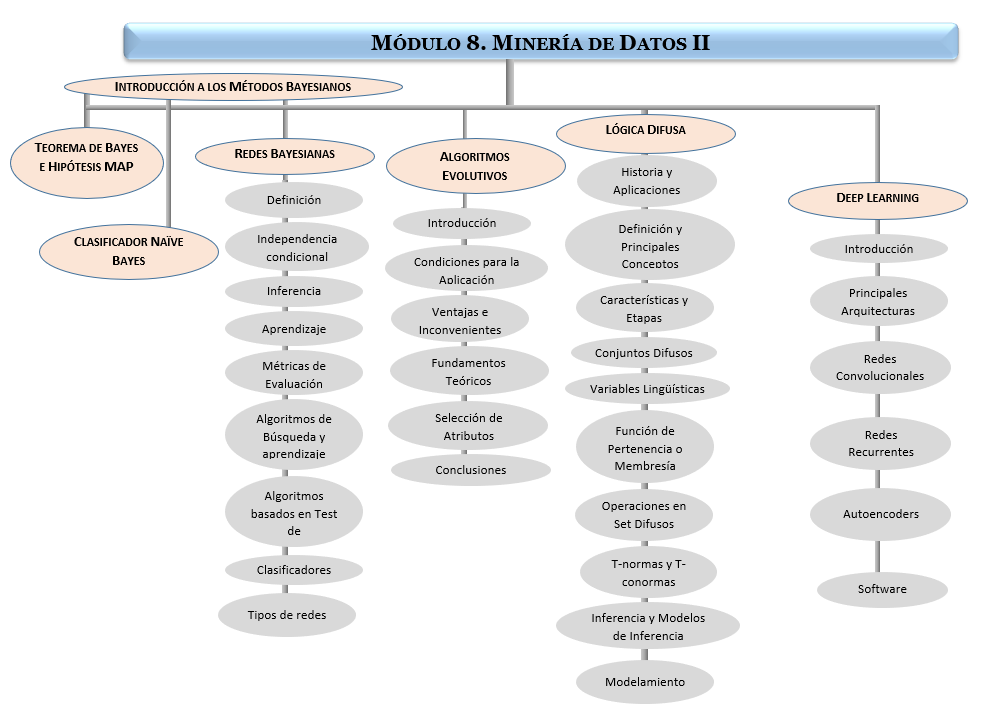
\includegraphics[width=1\textwidth,height=\textheight]{imagenes/diagrama_conceptual.png}

}

\caption{\label{fig-diagrama-conceptual}Diagrama Conceptual}

\end{figure}

\bookmarksetup{startatroot}

\hypertarget{deep-learning}{%
\chapter{Deep Learning}\label{deep-learning}}

\hypertarget{introducciuxf3n-1}{%
\section{Introducción}\label{introducciuxf3n-1}}

El \textbf{deep learning o aprendizaje profundo} es un concepto amplio,
un término de moda que atiende a una realidad que cada día está más
presente entre nosotros, y que no tiene una única definición que se
pueda considerar veraz, aunque podemos generalizar la definición
afirmando que surge de la idea de imitar el cerebro a partir de la
utilización de hardware y software, para crear inteligencia artificial.
Este intento de imitar al cerebro se ha plasmado en lo que se conoce
como redes neuronales artificiales (RNA) que están dotadas de una
capacidad de abstracción jerárquica: representan los datos de entrada en
varios ``niveles'', a través de arquitecturas en varias capas, cada capa
aprende patrones más complejos según la profundidad de ésta, para
conseguir información útil para el aprendizaje.

Podemos afirmar que el principio general del funcionamiento de una
arquitectura profunda es guiar el entrenamiento de las capas intermedias
utilizando aprendizaje no supervisado. Algunos de los prototipos de
arquitecturas y/o algoritmos desarrollados se basan en otras
arquitecturas ``más simples'', modificándolas y obteniendo una
arquitectura ``más profunda'', lo que quiere decir que en sus capas y
neuronas se separan las características de un conjunto de datos de
entrada de una forma jerarquizada.

Otra definición dada del aprendizaje profundo es que es un subconjunto
de los algoritmos usados en machine learning, y se caracterizan por
tener una \textbf{arquitectura en capas} donde cada capa aprende
patrones más complejos según la profundidad de ésta. En este sentido,
existen ya muchos prototipos de redes neuronales que tienen esta
característica, por ejemplo, las ya muy conocidas redes convolucionales
o las redes recurrentes. El Perceptron Multicapa de una sola capa
explicado en el módulo 5 no es considerado un método de aprendizaje
profundo. El Deep Learning es una técnica reciente donde aún se sigue
investigando y desarrollándose y que surgió a partir del año 2006, año
en el que se considera fue retomada su investigación. El principal
problema por el que se había ralentizado su progreso es que el
entrenamiento basado en el método del gradiente para redes neuronales
profundas supervisadas, según muchos investigadores, se estancaba en lo
que se llama mínimo local aparente, lo que significa que una red con más
capas ocultas, es decir una red neuronal más profunda, obtiene peores
resultados que una red con sólo una capa oculta. Los investigadores
abordaron este tema planteado a través de diferentes ópticas y se
descubre que se obtienen resultados más precisos si cada capa de la red
es entrenada a través de un algoritmo de preentrenamiento no supervisado
(el método del gradiente requiere que sea supervisado) Para el
entrenamiento de las capas, diversos autores sugieren utilizar
autoencoders o máquinas de Boltzmann y, una vez se hayan preentrenado
las diferentes capas, se puede aplicar un criterio supervisado. En estos
últimos años se ha producido un rápido crecimiento en la cantidad de
arquitecturas y/o algoritmos de entrenamiento en una RNA, incluso,
variantes de ellos, las cuales siguen el concepto planteado
anteriormente.

\hypertarget{revisiuxf3n-de-las-redes-neuronales}{%
\section{Revisión de las Redes
Neuronales}\label{revisiuxf3n-de-las-redes-neuronales}}

Vamos a hacer una revisión de las redes neuronales para posteriormente
poder abordar los diferentes tipos de redes neuronales que se utilizan
en Deep Learning. Algunos de los avances más recientes en varios de los
diferentes componentes que forman parte de las redes neuronales están
recopilados en (Gu et al.~2017) Las redes neuronales artificiales tienen
sus orígenes en el Perceptrón, que fue el modelo creado por Frank
Rosenblatt en 1957 y basado en los trabajos que previamente habían
realizado Warren McCullon (neurofisiólogo) y Walter Pitts (matemático).
El Perceptrón está construido por una neurona artificial cuyas entradas
y salida pueden ser datos numéricos, no como pasaba con la neurona de
McCulloch y Pitts (eran sólo datos lógicos). Las neuronas pueden tener
pesos y además se le aplica una función de activación Sigmoid (a
diferencia de la usada anteriormente al Paso binario). En esta neurona
nos encontramos que se realizan los siguientes cálculos:
\[ z = \sum_{i=1}^{n}w_ix_i+b_i\] \[\hat{y} = \delta (z)\]

donde representan los datos numéricos de entrada, son los pesos, es el
sesgo (bias), es la función de activación y finalmente es el dato de
salida. El modelo de perceptrón es el más simple, en el que hay una sola
capa oculta con una única neurona. El siguiente paso nos lleva al
Perceptrón Multicapa donde ya pasamos a tener más de una capa oculta, y
además podemos tener múltiples neuronas en cada capa oculta. Cuando
todas las neuronas de una capa están interconectadas con todas las de la
siguiente capa estamos ante una red neuronal densamente conectada. A lo
largo de las siguientes secciones nos encontraremos con redes en las que
no todas las neuronas de una capa se conectan con todas de la siguiente.
Veamos como describiríamos ahora los resultados de las capas donde
representan los datos de la neurona en la capa ( siendo los valores de
entrada), son los pesos en la capa , es el sesgo (bias) en la capa , es
la función de activación en la capa (puede que cada capa tenga una
función de activación diferente), es el número de neurona de la capa
anterior que conectan con la y finalmente es el dato de salida de la
capa . Es decir, en cada capa para calcular el nuevo valor necesitamos
usar los valores de la capa anterior.

\textbf{Aplicaciones de las Redes Neuronales}

Cada día las redes neuronales están más presentes en diferentes campos y
ayudan a resolver una gran variedad de problemas. Podríamos pensar que
de forma más básica una red neuronal nos puede ayudar a resolver
problemas de regresión y clasificación, es decir, podríamos considerarlo
como otro modelo más de los existentes que a partir de unos datos de
entrada somos capaces de obtener o un dato numérico (o varios) para
hacer una regresión (calcular en precio de una vivienda en función de
diferentes valores de la misma) o que somos capaces de conseguir que en
función de los datos de entrada nos deje clasificada una muestra
(decidir si conceder o no una hipoteca en función de diferentes datos
del cliente). Si los datos de entrada son imágenes podríamos estar
usando las redes neuronales como una forma de identificar esa imagen: •
Identificando que tipo de animal es • Identificando que señal de tráfico
es • Identificando que tipo de fruta es • Identificando que una imagen
es de exterior o interior de una casa • Identificando que es una cara de
una persona • Identificando que una imagen radiográfica represente un
tumor maligno • Identificando que haya texto en una imagen Luego
podríamos pasar a revolver problemas más complejos combinando las
capacidades anteriores: • Detectar los diferentes objetos y personas que
se encuentran en una imagen • Etiquedado de escenas (aula con alumnos,
partido de futbol, etc\ldots) Después podríamos dar el paso al video que
lo podríamos considerar como una secuencia de imágenes: • Contar el
número de personas que entran y salen de una habitación • Reconocer que
es una carretera • Identificar las señales de tráfico • Detectar si
alguien lleva un arma • Seguimiento de objetos • Detección de
estado/actitud de una persona • Reconocimiento de acciones (interpretar
lenguaje de signos, interpretar lenguaje de banderas) • Vehículos
inteligentes Si los datos de entrada son secuencias de texto • Sistemas
de traducción • Chatbots (resolución de preguntas a usuarios) •
Conversión de texto a audio Si los datos de entrada son audios •
Sistemas de traducción • Altavoces inteligentes • Conversión de audio a
texto

A continuación, pasamos a revisar diferentes elementos de las redes
neuronales que suelen ser comunes a todos los tipos de redes neuronales.

\textbf{Datos}

Cuando se trabaja con redes neuronales necesitamos representar los
valores de las variables de entrada en forma numérica. En una red
neuronal todos los datos son siempre numéricos. Esto significa que todas
aquellas variables que sean categóricas necesitamos convertirlas en
numéricas. Además, es muy conveniente normalizar los datos para poder
trabajar con valores entre 0 y 1, que van a ayudar a que sea más fácil
que se pueda converger a la solución. Es importante que los datos seán
números en coma flotante, sobre todo si se van a trabajar con GPUs
(Graphics Process Units), ya que permitirán hacer un mejor uso de los
multiples cores que les permiten operar en coma flotante de forma
paralela. Actualmente, hay toda una serie de mejoras en las GPUs que
permite aumentar el rendimiento de las redes neuronales como son el uso
de operaciones en FP16 (Floating Point de 16 bits en lugar de 32) de
forma que pueden hacer dos operaciones de forma simultánea (el formato
estándar es FP32) y además con la reducción de memoria (punto muy
importante) al meter en los 32 bits 2 datos en lugar de sólo uno.
También se han añadido técnicas de Mixed Precision (Narang et al.~2018),
los Tensor Cores (para las gráficas de NVIDIA) son otra de las mejoras
que se han ido incorporando a la GPUs y que permiten acelerar los
procesos tanto de entrenamiento como de predicción con las redes
neuronales.

El primer objetivo será convertir las variables categóricas en variables
numéricas, de forma que el AE pueda trabajar con ellas. Para realizar la
conversión de categórica a numérica básicamente tenemos dos métodos para
realizarlo: • Codificación one-hot. • Codificación entera. La
codificación one-hot consiste en crear tantas variables como categorías
tenga la variable, de forma que se asigna el valor 1 si tiene esa
categoría y el 0 si no la tiene.

La codificación entera lo que hace es codificar con un número cada
categoría. Realmente esta asignación no tiene ninguna interpretación
numérica ya que en general las categorías no tienen porque representar
un orden al que asociarlas. Normalmente se trabaja con codificación
one-hot para representar los datos categóricos de forma que será
necesario preprocesar los datos de partida para realizar esta
conversión, creando tantas variables como categorías haya por cada
variable. Si nosotros tenemos nuestra muestra de datos de que tiene
variables de forma que , y son variables categóricas que tienen número
de categorías respectivamente, tendremos finalmente las siguientes
variables sólo numéricas:

De esta forma, se aumentarán el número de variables con las que vamos a
trabajar en función de las categorías que tengan las variables
categóricas. Normalmente nos encontramos que en una red neuronal las
variables de salida son: • un número (regresión) • una serie de números
(regresión múltiple) • un dato binario (clasificación binaria) • una
serie de datos binarios que representa una categoría de varias
(clasifiación múltiple)

\textbf{Arquitectura de red}

Para la construcción de una red neuronal necesitamos definir la
arquitectura de esa red. Esta arquitectura, si estamos pensando en una
red neuronal densamente conectada, estará definida por la cantidad de
capas ocultas y el número de neuronas que tenemos en cada capa. Más
adelante veremos que dependiendo del tipo de red neuronal podrá haber
otro tipo de elementos en estas capas. Función de coste y pérdida Otro
de los elementos clave que tenemos que tener en cuenta a la hora de usar
nuestra red neuronal son las funciones de pérdida y funciones de coste
(objetivo). La función de pérdida va a ser la fución que nos dice cómo
de diferente es el resultado del dato que nosotros queríamos conseguir
respecto al dato original. Normalmente se suelen usar diferentes tipos
de funciones de pérdida en función del tipo de resultado con el que se
vaya a trabajar. La función de coste es la función que vamos a tener que
optimizar para conseguir el mínimo valor posible, y que recoge el valor
de la función de pérdida para toda la muestra. Tanto las funciones de
pérdida como las funciones de coste, son funciones que devuelven valores
de .

Si tenemos un problema de regresión en el que tenemos que predecir un
valor o varios valores numéricos, algunas de las funciones a usar son: •
Error medio cuadrático () {[}120{]} , es el valor real e es el valor
predicho • Error medio absoluto () {[}121{]} , es el valor real e es el
valor predicho Para los problemas de clasifiación: • Binary Crossentropy
(Sólo hay dos clases) {[}122{]} es el valor real e es el valor predicho
• Categorical Crosentropy (Múltiples clases representadas como one-hot)
{[}123{]} es el valor real para la clase e es el valor predicho para la
clase • Sparse Categorical Crossentropy (Múltiples clases representadas
como un entero) {[}124{]} es el valor real para la clase e es el valor
predicho para la clase • Kullback-Leibler Divergence Esta función se usa
para calcular la diferencia entre dos distribuciones de probabilidad y
se usa por ejemplo en algunas redes como Variational Autoencoders
(Doersch 2016) o Modelos GAN (Generative Adversarial Networks) {[}125{]}
{[}126{]} {[}127{]} • Hinge Loss {[}128{]} Las correspondientes
funciones de coste que se usarían, estarían asociadas a todas las
muestras que se estén entrenando o sus correpondientes batch, así como
posibles términos asociados a la regularización para evitar el
sobreajuste del entrenamiento. Es decir, la función de pérdida se
calcula para cada muestra, y la función de coste es la media de todas
las muestras. Por ejemplo, para el Error medio cuadrático () tendríamos
el siguiente valor: {[}129{]}

\textbf{Optimizador}

El Descenso del gradiente es la versión más básica de los algoritmos que
permiten el aprendizaje en la red neuronal haciendo el proceso de
backpropagation (propagación hacia atrás). A continuación veremos una
breve explicación del algoritmo así como algunas variantes del mismo
recogidas en (Ruder 2017) Recordamos que el descenso del gradiente nos
permitirá actualizar los parámetros de la red neuronal cada vez que
demos una pasada hacia delante con todos los datos de entrada, volviendo
con una pasada hacia atrás. {[}130{]} donde es la función de coste, es
el parámetro de ratio de aprendizaje que permite definir como de grandes
se quiere que sean los pasos en el aprendizaje. Cuando lo que hacemos es
actualizar los parámetros para cada pasada hacia delante de una sola
muestra, estaremos ante lo que llamamos Stochastic Gradient Descent
(SGD). En este proceso convergerá en menos iteraciones, aunque puede
tener alta varianza en los parámetros. {[}131{]} donde e son los valores
en la pasada de la muestra . Podemos buscar un punto intermedio que
sería cuando trabajamos por lotes y cogemos un bloque de datos de la
muestra, les aplicamos la pasada hacia delante y aprendemos los
parámetros para ese bloque. En este caso lo llamaremos Mini-batch
Gradient Descent {[}132{]} donde son los valores de ese batch . En
general a estos métodos nos referiremos a ellos como SGD. Sobre este
algoritmo base se han hecho ciertas mejoras como: \textbf{Learning rate
decay} Podemos definir un valor de decenso del ratio de aprendizaje, de
forma que normalmente al inicio de las iteraciones de la red neuronal
los pasos serán más grandes, pero conforme nos acercamos a la solución
optima deberemos dar pasos más pequeños para ajustarnos mejor. {[}133{]}
donde ahora se irá reduciendo en función del valor del decay Momentum El
\textbf{momentum} se introdujo para suavizar la convergencia y reducir
la alta varianza de SGD. {[}134{]} {[}135{]} donde es lo que se llama el
vector velocidad con la dirección correcta. \textbf{NAG (Nesterov
Accelerated Gradient)} Ahora daremos un paso más con el NAG, calculando
la función de coste junto con el vector velocidad. {[}136{]} {[}137{]}
donde ahora vemos que la función de coste se calcula usando los
parámetros de sumado a

Veamos algunos algoritmos de optimización más que, aunque provienen del
SGD, se consideran independientes a la hora de usarlos y no como
parámetros extras del SGD. \textbf{Adagrad (Adaptive Gradient)} Esta
variante del algoritmo lo que hace es adaptar el ratio de aprendizaje
para cada uno de los pesos en lugar de que sea global para todos.
{[}138{]} donde tenemos que es una matriz diagonal donde cada elemento
es la suma de los cuadrados de los gradientes en el paso , y es un
término de suavizado par evitar divisiones por 0.

\textbf{RMSEProp (Root Mean Square Propagation)} En este caso tenemos
una variación del Adagrad en el que intenta reducir su agresividad
reduciendo monotonamente el ratio de aprendizaje. En lugar de usar el
gradiente acumulado desde el principio de la ejecución, se restringe a
una ventana de tamaño fijo para los últimos n gradientes calculando su
media. Así calcularemos primero la media en ejecución de los cuadros de
los gradientes como: {[}139{]} y luego ya pasaremos a usar este valor en
la actualización {[}140{]}

\textbf{AdaDelta}

Aunque se desarrollaron de forma simultánea el AdaDelta y el RMSProp son
muy parecidos en su primer paso incial, llegando el de AdaDelta un poco
más lejos en su desarrollo. {[}141{]} y luego ya pasaremos a usar este
valor en la actualización {[}142{]} {[}143{]} \textbf{Adam (Adaptive
Moment Estimation)} {[}144{]} {[}145{]} {[}146{]} donde y son
estimaciones del primer y segundo momento de los gradientes
respectivamente, y y parámetros a asignar. {[}147{]} {[}148{]} {[}149{]}
\textbf{Adamax} {[}150{]} {[}151{]} {[}152{]} {[}153{]} donde y son
estimaciones del primer y segundo momento de los gradientes
respectivamente, y y parámetros a asignar. {[}154{]} {[}155{]}
\textbf{Nadam (Nesterov-accelerated Adaptive Moment Estimatio)} Combina
Adam y NAG. {[}156{]} {[}157{]} {[}158{]}

\textbf{Función de activación} Las funciones de activación dentro de una
red neuronal son uno de los elementos clave en el diseño de la misma.
Cada tipo de función de activación podrá ayudar a la convergencia de
forma más o menos rápida en función del tipo de problema que se plantee.
En un AE las funciones de activación en las capas ocultas van a
conseguir establecer las restricciones no lineales al pasar de una capa
a la siguiente, normalmente se evita usar la función de activación
lineal en las capas intermedias ya que queremos conseguir
transformaciones no lineales. A continuación, exponemos las principales
funciones de activación que mejores resultados dan en las capas ocultas:
• Paso binario (Usado por los primeros modelos de neuronas) {[}159{]} •
Identidad {[}160{]} • Sigmoid (Logística) {[}161{]} • Tangente
Hiperbólica (Tanh) {[}162{]} • Softmax {[}163{]}

\begin{verbatim}
• ReLu ( Rectified Linear Unit)
    [164]

• LReLU (Leaky Rectified Linear Unit)
    [165]
• PReLU (Parametric Rectified Linear Unit)
    [166]
• RReLU (Randomized Rectified Linear Unit)
    [167]
\end{verbatim}

*La diferencia entre LReLu, PReLu y RRLeLu es que en LReLu el parámetro
es uno que se asigna fijo, en el caso de PReLu el parámetro también se
aprende durante el entrenamiento y finalmente en RReLu es un parámetro
con valores entre 0 y 1, que se obtiene de un muestreo en una
distribución normal. Se puede profundizar en este grupo de funciones de
activación en (Xu et al.~2015) • ELU (Exponential Linear Unit) {[}168{]}
FIGURA nº 64: COMPARACIÓN ENTRE LAS FUNCIONES ReLU, LReLU/PReLU, RReLU y
ELU

FUENTE: Jiuxiang, G. et al (2019)

\textbf{Función de activación en salida} En la capa de salida tenemos
que tener en cuenta cual es el tipo de datos final que queremos obtener,
y en función de eso elegiremos cual es la función de activación de
salida que usaremos. Normalmente las funciones de activación que se
usarán en la última capa seran: • Lineal con una unidad, para regresión
de un solo dato numérico {[}169{]} donde es un valor escalar. • Lineal
con multiples unidades, para regresión de varios datos numéricos
{[}170{]} donde es un vector. • Sigmoid para clasifiación binaria
{[}171{]} • Softmax para calsifiación múltiple {[}172{]}

\textbf{Regularización} Las técnicas de regularización nos permiten
conseguir mejorar los problemas que tengamos por sobreajuste en el
entrenamiento de nuestra red neuronal. A continuación, vemos algunas de
las técnicas de regularización existentes en la actualidad: • Norma LP
Básicamente estos métodos tratan de hacer que los pesos de las neuronas
tengan valores muy pequeños consiguiendo una distribución de pesos más
regular. Esto lo consiguen al añadir a la función de pérdida un coste
asociado a tener pesos grandes en las neuronas. Este peso se puede
construir o bien con la norma L1 (proporcional al valor absoluto) o con
la norma L2 (proporcional al cuadrado de los coeficientes de los pesos).
En general se define la norma LP) {[}173{]} {[}174{]} Para los casos más
habituales tendríamos la norma L1 y L2. {[}175{]} {[}176{]}

\textbf{Dropout} Una de las técnicas de regularización que más se están
usando actualmente es la llamada Dropout, su proceso es muy sencillo y
consiste en que en cada iteración de forma aleatoria se dejan de usar un
porcentaje de las neuronas de esa capa, de esta forma es más dificil
conseguir un sobreajuste porque las neuronas no son capaces de memorizar
parte de los datos de entrada. \textbf{Dropconnect} El Dropconnect es
otra técnica que va un poco más allá del concepto de Dropout y en lugar
de usar en cada capa de forma aleatoria una serie de neuronas, lo que se
hace es que de forma aleatoria se ponen los pesos de la capa a cero. Es
decir, lo que hacemos es que hay ciertos enlaces de alguna neurona de
entrada con alguna de salida que no se activan.

\textbf{Inicialización de pesos}

Cuando empieza el entrenamiento de una red neuronal y tiene que realizar
la primera pasada hacia delante de los datos, necesitamos que la red
neuronal ya tenga asignados algún valor a los pesos. Se pueden hacer
inicializaciones del tipo: • Ceros Todos los pesos se inicializan a 0. •
Unos Todos los pesos se inicializan a 1. • Distribución normal Los pesos
se inicializan con una distribución normal, normalmente con media 0 y
una desviación alrededor de 0,05. Es decir, valores bastante cercanos al
cero. • Distribución normal truncada Los pesos se inicializan con una
distribución normal, normalmente con media 0 y una desviación alrededor
de 0,05 y además se truncan con un máximo del doble de la desviación.
Los valores aun són más cercanos a cero. • Distribución uniforme Los
pesos se inicializan con una distribución uniforme, normalmente entre el
0 y el 1. • Glorot Normal (También llamada Xavier normal) Los pesos se
inicializan partiendo de una distribución normal truncada en la que la
desivación es donde es el número de unidades de entrada y fanout es el
número de unidades de salida. Ver (Glorot and Bengio 2010) • Glorot
Uniforme (También llamada Xavier uniforme) Los pesos se inicializan
partiendo de una distribución uniforme done los límites son done y es el
número de unidades de entrada y fanout es el número de unidades de
salida. Ver (Glorot and Bengio 2010)

\textbf{Batch normalization} Hemos comentado que cuando entrenamos una
red neuronal los datos de entrada deben ser todos de tipo numérico y
además los normalizamos para tener valores ``cercanos a cero'', teniendo
una media de 0 y varianza de 1, consiguiendo uniformizar todas las
variables y conseguir que la red pueda converger más fácilmente. Cuando
los datos entran a la red neuronal y se comienza a operar con ellos, se
convierten en nuevos valores que han perdido esa propiedad de
normalización. Lo que hacemos con la normalización por lotes (batch
normalization) (Ioffe and Szegedy 2015) es que añadimos un paso extra
para normalizar las salidas de las funciones de activación. Lo normal es
que se aplicara la normalización con la media y la varianza de todo el
bloque de entrenamiento en ese paso, pero normalmente estaremos
trabajando por lotes y se calculará la media y varianza con ese lote de
datos.

\hypertarget{principales-arquitecturas-de-deep-learning}{%
\subsection{Principales arquitecturas de Deep
Learning}\label{principales-arquitecturas-de-deep-learning}}

Actualmente existen muchos tipos de estructuras de redes neuronales
artificiales dado que logran resultados extraordinarios en muchos campos
del conocimiento. Los primeros éxitos en el aprendizaje profundo se
lograron a través de las investigaciones y trabajos de Geoffre Hinton
(2006) que introduce las Redes de Creencia Profunda en cada capa de la
red de una Máquina de Boltzmann Restringida (RBM) para la asignación
inicial de los pesos sinápticos. Hace tiempo que se está trabajando con
arquitecturas como los Autoencoders, Hinton y Zemel (1994), las RBMs de
Hinton y Sejnowski (1986) y las DBNs (Deep Belief Networks), Hinton et
al.~(2006) y otras como las redes recurrentes y convolucionales. Estas
técnicas constituyen en sí mismas arquitecturas de redes neuronales,
aunque también algunas de ellas, como se ha afirmado en la introducción,
se están empleando para inicializar los pesos de arquitecturas profundas
de redes neuronales supervisadas con conexiones hacia adelante. Las
principales arquitecturas de deep learning se resumen en la siguiente
figura. Figura 65. modelos de redes neuronales según tipo de aprendizaje

Vamos a describir de forma somera las principales arquitecturas dado que
posteriormente se desarrollan más ampliamente en este epígrafe o se
tratan en docuemento adjunto que se acompaña en este módulo
\textbf{Convolutional Neural Network} Tal vez los modelos más utilizados
actualmente en el campo del Deep Learning sean las redes neuronales
convolucionales, denominadas en inglés Convolutional Neural Networks
(CNN). El objetivo de las redes CNN es aprender características de orden
superior utilizando la operación de convolución. Estas estructuras de
redes neuronales son especialmente eficaces para clasificar y segmentar
imágenes, en general, son notablemente eficaces en tareas de visión
artificial. Las CNN son una modificación del perceptrón multicapa
explicado en un módulo anterior. Este modelo es muy similar al trabajo
que ejecuta el cerebro humano: las neuronas se corresponden a campos
receptivos similares a como lo realizan las neuronas en la corteza
visual de nuestro cerebro. Esta arquitectura ya se utilizó en 1990 donde
la empresa AT \& T las aplicó para crear un modelo de lectura de
cheques, desarrollándose posteriormente muchos sistemas OCR basados en
CNN. Las redes de convolución tienen una estructura de varias capas: las
capas de Convolución que transforman los datos de entrada a través de
una operación matemática llamada Convolución y la capa de pooling, que
trata de sintetizar y condensar la información de la capa de
convolución. Finalmente, se transforman los datos para aplicar una red
densamente conectada que nos ofrece el resultado final en relación con
el objetivo que se busca. Estas redes neuronales artificiales se
desarrollaron al abrigo de los concursos denominados ILSVRC (Large Scale
Visual Recognition Challenge) donde aparecieron las principales
aportaciones efectuadas en las redes convolucionales y que hoy podemos
utilizar todos los investigadores. Algunos de las estructuras más
novedosas y que son modelos ya preentrenados, con estructuras de capas
más numerosas y que podemos integrar en nuestras aplicaciones, se
denominan: LeNet-5, AlexNet, VGG, GoogLeNet y Resnet.

\textbf{Autoencoder} Los Autoencoders (AE) son uno de los tipos de redes
neuronales que caen dentro del ámbito del Deep Learning, en la que nos
encontramos con un modelo de aprendizaje no supervisado. Ya se empezó a
hablar de AE en la década de los 80 (Bourlard and Kamp 1988), aunque es
en estos últimos años donde más se está trabajando con ellos. La
arquitectura de un AE es una Red Neuronal Artificial (ANN por sus siglas
en inglés) que se encuentra dividida en dos partes, encoder y decoder
(Charte et al.~2018), (Goodfellow, Bengio, and Courville 2016). El
encoder va a ser la parte de la ANN que va codificar o comprimir los
datos de entrada, y el decoder será el encargado de regenerar de nuevo
los datos en la salida. Esta estructura de codificación y decodificación
le llevará a tener una estructura simétrica. El AE es entrenado para ser
capaz de reconstruir los datos de entrada en la capa de salida de la
ANN, implementando una serie de restricciones (la reducción de elementos
en las capas ocultas del encoder) que van a evitar que simplemente se
copie la entrada en la salida. Algunas de sus principales aplicaciones
sobre las que se está investigando son: • Reducción de dimensiones /
Compresión de datos • Búsqueda de imágenes • Detección de Anomalías •
Eliminación de ruido \textbf{Redes recurrentes} En la actualidad las
\textbf{redes neuronales recurrentes (Recurrent Neural Networks)} han
logrado un puesto destacado en machine learning. Estas redes que no
disponen de una estructura de capas, sino que permiten conexiones
arbitrarias entre todas las neuronas, incluso creando ciclos. En esta
arquitectura se permiten conexiones recurrentes lo que aumenta el número
de pesos o de parámetros ajustables de la red, lo que incrementa la
capacidad de representación, pero también la complejidad del
aprendizaje. Las peculiaridades de esta red permiten incorporar a la red
el concepto de temporalidad, y también que la red tenga memoria, porque
los números que introducimos en un momento dado en las neuronas de
entrada son transformados, y continúan circulando por la red. Existen
diferentes planteamientos de redes recurrentes, por ejemplo, son muy
populares por sus aplicaciones las redes de Elmann y de Jordan. En los
últimos años se han popularizado las redes recurrentes denominadas
Long-Short Term Memory (LSTM) que son una extension de las redes
recurrentes y su caracterítica principal es que amplian su memoria para
registrar experiencias que han ocurrido hace mucho tiempo. Normalmente
contienen tres puertas que determinan si se permite o no una nueva
entrada o se elimina la información que llega dado que se considera no
importante. Son análogas a una función sigmoide lo que implica que van
de 0 a 1, lo que permite incorporarlas al proceso de backpropagation.
También se encuentran entre las redes recurrentes, las denominadas GRU
(Gated Recurrent Unit) que aparecieron en 2014 y simplifican a las LSMT:
son computacionalmente menos costosas y más eficientes.

Boltzmann Machine y Restricted Boltzmann Machine El aprendizaje de la
denominada máquina de Boltzmann (BM) se realiza a través de un algoritmo
estocástico que proviene de ideas basadas en la mecánica estadística.
Este prototipo de red neuronal tiene una característica distintiva y es
que el uso de conexiones sinápticas entre las neuronas es simétrico. Las
neuronas son de dos tipos: visibles y ocultas. Las neuronas visibles son
las que interactúan y proveen una interface entre la red y el ambiente
en el que operan, mientras que las neuronas actúan libremente sin
interacciones con el entorno. Esta máquina dispone de dos modos de
operación. El primero es la condición de anclaje donde las neuronas
están fijas por los estímulos específicos que impone el ambiente. El
otro modo es la condición de libertad, donde tanto las neuronas ocultas
como las visibles actúan libremente sin condiciones impuestas por el
medio ambiente. Las maquinas restringidas de Boltzmann (RBM) solamente
toman en cuenta aquellos modelos en los que no existen conexiones del
tipo visible-visible y oculta-oculta. Estas redes también asumen que los
datos de entrenamiento son independientes y están idénticamente
distribuidos. Una forma de estimar los parámetros de un modelo
estocástico es calculando la máxima verosimilitud. Para ello, se hace
uso de los Markov Random Fiels (MRF), ya que al encontrar los parámetros
que maximizan los datos de entrenamiento bajo una distribución MRF,
equivale a encontrar los parámetros 𝜃 que maximizan la verosimilitud de
los datos de entrenamiento, Fischer e Igel (2012). Maximizar dicha
verosimilitud es el objetivo que persigue el algoritmo de entrenamiento
de una RBM. A pesar de utilizar la distribución MRF, computacionalmente
hablando se llega a ecuaciones inviables de implementar. Para evitar el
problema anterior, las esperanzas que se obtienen de MRF pueden ser
aproximadas por muestras extraídas de distribuciones basadas en las
técnicas de Markov Chain Monte Carlo Techniques (MCMC). Las técnicas de
MCMC utilizan un algoritmo denominado muestreo de Gibbs con el que
obtenemos una secuencia de observaciones o muestras que se aproximan a
partir de una distribución de verosimilitud de múltiples variables
aleatorias. La idea básica del muestreo de Gibss es actualizar cada
variable posteriormente en base a su distribución condicional dado el
estado de las otras variables. Deep Belief Network Una red Deep Belief
Network tal como demostró Hinton se puede considerar como un
``apilamiento de redes restringidas de Boltzmann''. Tiene una estructura
jerárquica que como sabemos es una de las características del deep
learning. Como en el anterior modelo, esta red también es un modelo en
grafo estocástico, que aprende a extraer una representación jerárquica
profunda de los datos de entrenamiento. Cada capa de la RBM extrae un
nivel de abstracción de características de los datos de entrenamiento,
cada vez más significativo; pero para ello, la capa siguiente necesita
la información de la capa anterior lo que implica el uso de las
variables latentes. Estos modelos caracterizan la distribución conjunta
hk entre el vector de observaciones x y las capas ocultas, donde x=h0,
es una distribución condicional para las unidades visibles limitadas
sobre las unidades ocultas que pertenecen a la RBM en el nivel k, y es
la distribución conjunta oculta visible en la red RBM del nivel superior
o de salida. El entrenamiento de esta red puede ser híbrido, empezando
por un entrenamiento no supervisado para después aplicar un
entrenamiento supervisado para un mejor y más óptimo ajuste, aunque
pueden aplicarse diferentes tipos de entrenamiento, Bengio et al.~(2007)
y Salakhutdinov (2014) Para realizar un entrenamiento no supervisado se
aplica a las redes de creencia profunda con Redes restringidas de
Boltzmann el método de bloque constructor que fue presentado por Hinton
(2006) y por Bengio (2007)

\hypertarget{redes-neuronales-convolucionales}{%
\section{Redes Neuronales
Convolucionales}\label{redes-neuronales-convolucionales}}

\hypertarget{introducciuxf3n-2}{%
\subsection{Introducción}\label{introducciuxf3n-2}}

Esta arquitectura de redes de neuronas convolucionales, CNN,
Convolutional Neural Networks es en la actualidad el campo de
investigación más fecundo dentro de las redes neuronales artificiales de
Deep learning y donde los investigadores, empresas e instituciones están
dedicando más recursos e investigación. Para apoyar esta aseveración, en
google trend se observa que el término convolutional neural network en
relación con el concepto de artificial neural network crece y está por
encima desde el año 2016. Es en este último lustro donde el Deep
learning ha tomado una importancia considerable.

\begin{figure}

{\centering 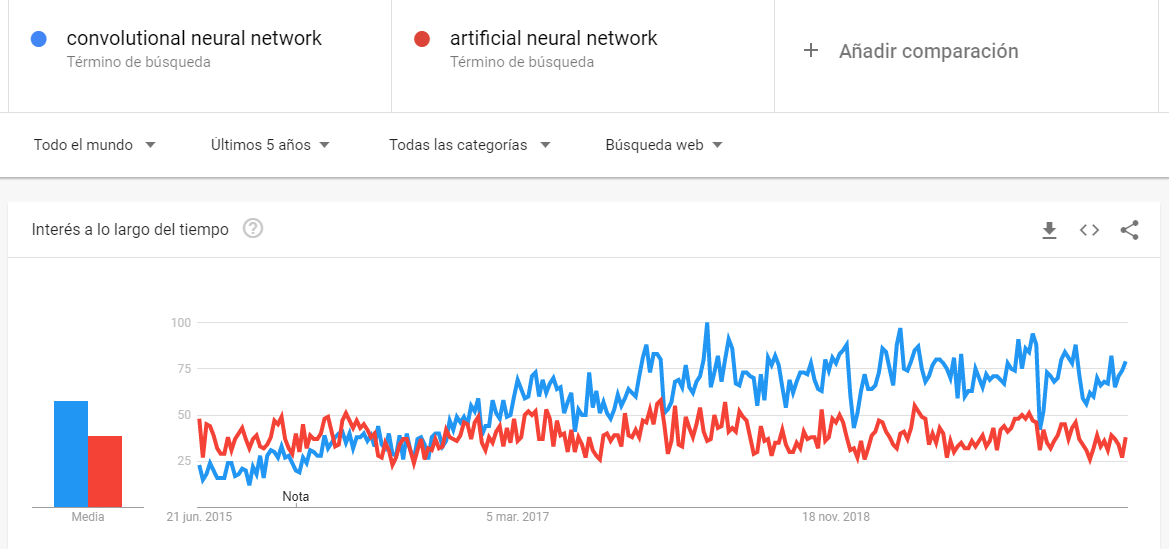
\includegraphics{imagenes/capitulo1/busqueda_google.png}

}

\caption{\label{fig-busqueda-google}búsqueda de términos de redes
neuronales en google trend}

\end{figure}

Fuente: Google Trend En este modelo de redes convolucionales las
neuronas se corresponden a campos receptivos similares a las neuronas en
la corteza visual de un cerebro humano. Este tipo de redes se han
mostrado muy efectivas para tareas de detección y categorización de
objetos y en la clasificación y segmentación de imágenes. Por ejemplo,
estas redes en la década de 1990 las aplicó AT \& T para desarrollar un
modelo para la lectura de cheques. También más tarde se desarrollaron
muchos sistemas OCR basados en CNN. En esta arquitectura cada neurona de
una capa no recibe conexiones entrantes de todas las neuronas de la capa
anterior, sino sólo de algunas. Esta estrategia favorece que una neurona
se especialice en una región del conjunto de números (píxeles) de la
capa anterior, lo que disminuye notablemente el número de pesos y de
operaciones a realizar. Lo más normal es que neuronas consecutivas de
una capa intermedia se especialicen en regiones solapadas de la capa
anterior. Una forma intuitiva para entender cómo trabajan estas redes
neuronales es ver cómo nos representamos y vemos las imágenes. Para
reconocer una cara primero tenemos que tener una imagen interna de lo
que es una cara. Y a una imagen de una cara la reconocemos porque tiene
nariz, boca, orejas, ojos, etc. Pero en muchas ocasiones una oreja está
tapada por el pelo, es decir, los elementos de una cara se pueden
ocultar de alguna manera. Antes de clasificarla, tenemos que saber la
proporción y disposición y también cómo se relacionan la partes entre
sí. Para saber si las partes de la cara se encuentran en una imagen
tenemos que identificar previamente líneas bordes, formas, texturas,
relación de tamaño, etcétera. En una red convolucional, cada capa lo que
va a ir aprendiendo son los diferentes niveles de abstracción de la
imagen inicial. Para comprender mejor el concepto anterior hemos
seleccionado esta imagen de Raschka y Mirjalili (2019) donde se observa
como partes del perro se transforman en neuronas del mapa de
características

\begin{figure}

{\centering 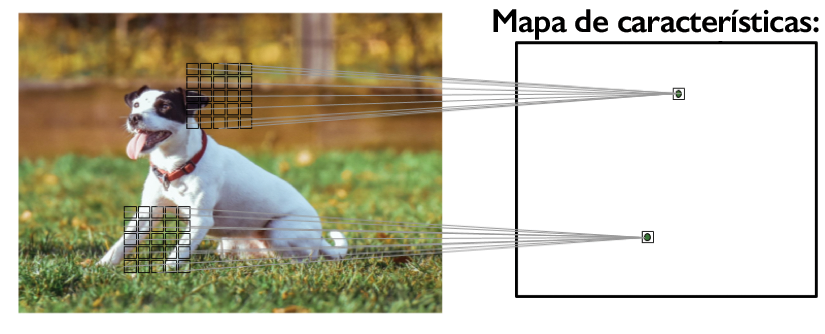
\includegraphics{imagenes/capitulo1/correspondencia_featrures.png}

}

\caption{\label{fig-correspondencia-features}Correspondencia de zonas de
la imagen y mapa de características}

\end{figure}

Fuente: Raschka y Mirjalili (2019)

El objetivo de las redes CNN es aprender características de orden
superior utilizando la operación de convolución. Puesto que las redes
neuronales convolucionales pueden aprender relaciones de entrada-salida
(donde la entrada es una imagen), en la convolución, cada pixel de
salida es una combinación lineal de los pixeles de entrada. La
convolución consiste en filtrar una imagen utilizando una máscara.
Diferentes máscaras producen distintos resultados. Las máscaras
representan las conexiones entre neuronas de capas anteriores. Estas
capas aprenden progresivamente las características de orden superior de
la entrada sin procesar. Las redes neuronales convolucionales se forman
usando dos tipos de capas: convolucionales y pooling. La capa de
convolución transforma los datos de entrada a través de una operación
matemática llamada convolución. Esta operación describe cómo fusionar
dos conjuntos de información diferentes. A esta operación se le suele
aplicar una función de transformación, generalmente la RELU. Después de
la capa o capas de convolución se usa una capa de pooling, cuya función
es resumir las respuestas de las salidas cercanas. Antes de obtener el
output unimos la última capa de pooling con una red densamente
conectada. Previamente se ha aplanado (Flatering) la última capa de
pooling para obtener un vector de entrada a la red neural final que nos
ofrecerá los resultados.

\begin{figure}

{\centering 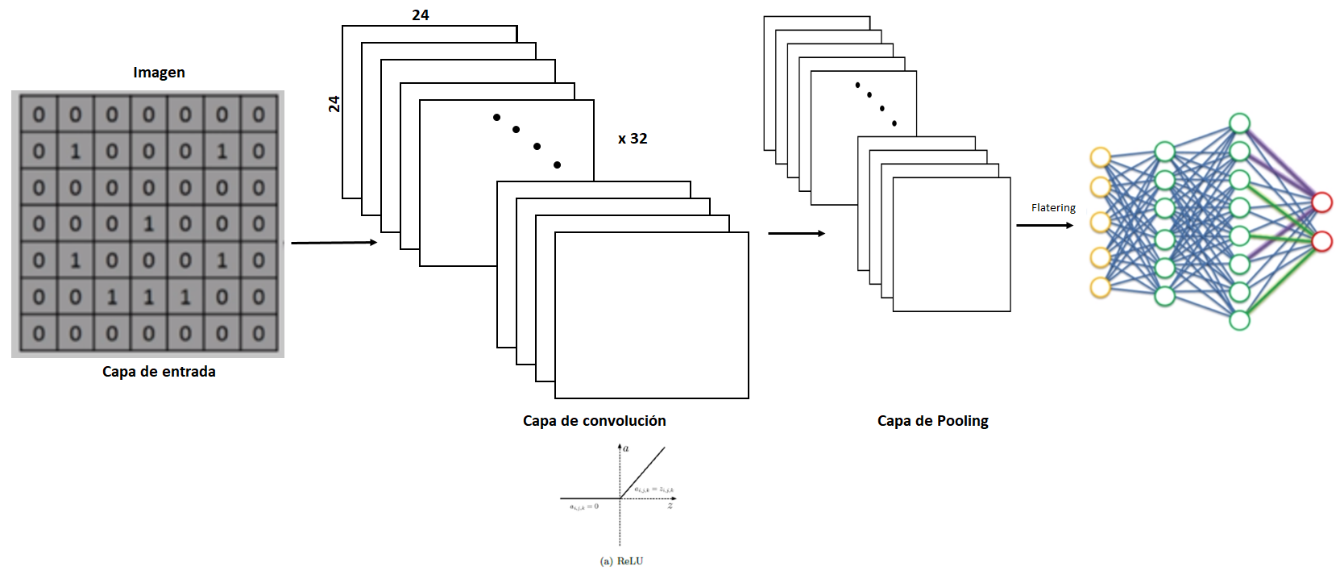
\includegraphics{imagenes/capitulo1/arquitectura_convolucional.png}

}

\caption{\label{fig-arquitectura_convolucional}Arquitectura de una CNN}

\end{figure}

Las redes neuronales convolucionales debido a su forma de concebirse son
aptas para poder aprender a clasificar todo tipo de datos donde éstos
estén distribuidos de una forma continua a lo largo del mapa de entrada,
y a su vez sean estadísticamente similares en cualquier lugar del mapa
de entrada. Por esta razón, son especialmente eficaces para clasificar
imágenes. También pueden ser aplicadas para la clasificación de series
de tiempo o señales de audio. En relación con el color y la forma de
codificarse, en las redes convolucionales se realiza en tensores 3D, dos
ejes para el ancho (width) y el alto (height) y el otro eje llamado de
profundidad (depht) que es el canal del color con valor tres si
trabajamos con imágenes de color RGB (Red, Green y Blue) rojo, verde y
azul. Si disponemos de imágenes en escala de grises el valor de depht es
uno. La base de datos MNIST (National Institute of Standards and
Technology database) con la que trabajaremos en este epígrafe contiene
imágenes de 28 x 28 pixeles, los valores de height y de widht son ambos
28, y al ser una base de datos en blanco y negro el valor de depht es 1.
Las imágenes son matrices de píxeles que van de cero a 255 y que para la
red neuronal se normalizan para que sus valores oscilen entre cero y
uno. 7.4.2. Convolución En las redes convolucionales todas las neuronas
de la capa de entrada (los píxeles de las imágenes) no se conectan con
todas las neuronas de la capa oculta del primer nivel como lo hacen las
redes clásicas del tipo perceptrón multicapa o las redes que conocemos
de forma genérica como redes densamente conectadas. Las conexiones se
realizan por pequeñas zonas de la capa de entrada.

\begin{figure}

{\centering 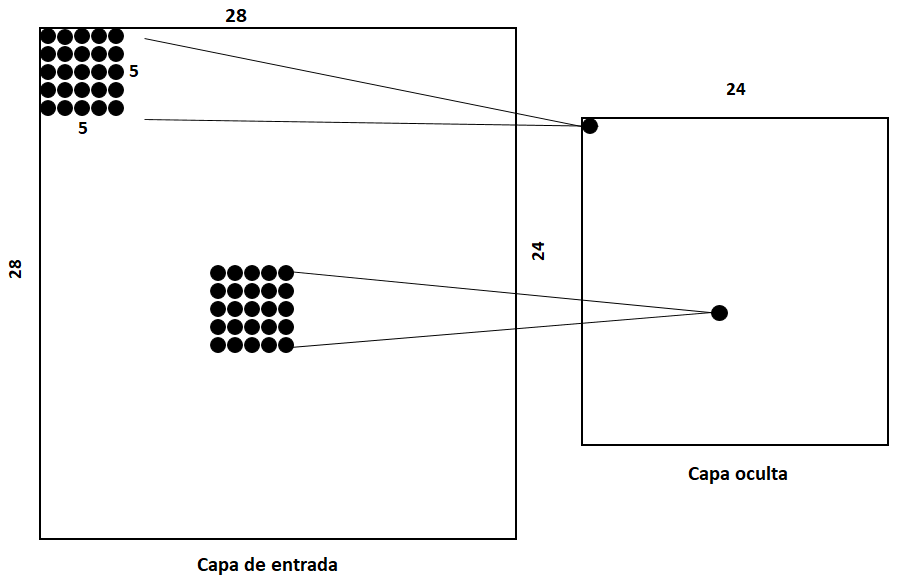
\includegraphics{imagenes/capitulo1/conexion_neuronas_convolucional.png}

}

\caption{\label{fig-conexion-neuronas-convolucional}Conexión de las
neuronas de la capa de entrada con la capa oculta}

\end{figure}

Veamos un ejemplo para la base de datos de los dígitos del 1 a 9. Vamos
a conectar cada neurona de la capa oculta con una región de 5 x 5
neurona, es decir, con 25 neuronas de la capa de entrada, que podemos
denominarla ventana. Esta ventana va a ir recorriendo todo el espacio de
entrada de 28 x 28 empezando por arriba y desplazándose de izquierda a
derecha y de arriba abajo. Suponemos que los desplazamientos de la
ventana son de un paso (un pixel) aunque este es un parámetro de la red
que podemos modificar (en la programación lo llamaremos stride). Para
conectar la capa de entrada con la de salida utilizaremos una matriz de
pesos (W) de tamaño 3 x 3 que recibe el nombre de filtro (filter) y el
valor del sesgo. Para obtener el valor de cada neurona de la capa oculta
realizaremos el producto escalar entre el filtro y la ventana de la capa
de entrada. Utilizamos el mismo filtro para obtener todas las neuronas
de la capa oculta, es decir en todos los productos escalares siempre
utilizamos la misma matriz, el mismo filtro. Se definen matemáticamente
estos productos escalares a través de la siguiente expresión: {[}177{]}

Como en este tipo de red un filtro sólo nos permite revelar una
característica muy concreta de la imagen, lo que se propone es usar
varios filtros simultáneamente, uno para cada característica que
queramos detectar. Una forma visual de representarlo (si suponemos que
queremos aplicar 32 filtros) es como se muestra a continuación:

\begin{figure}

{\centering 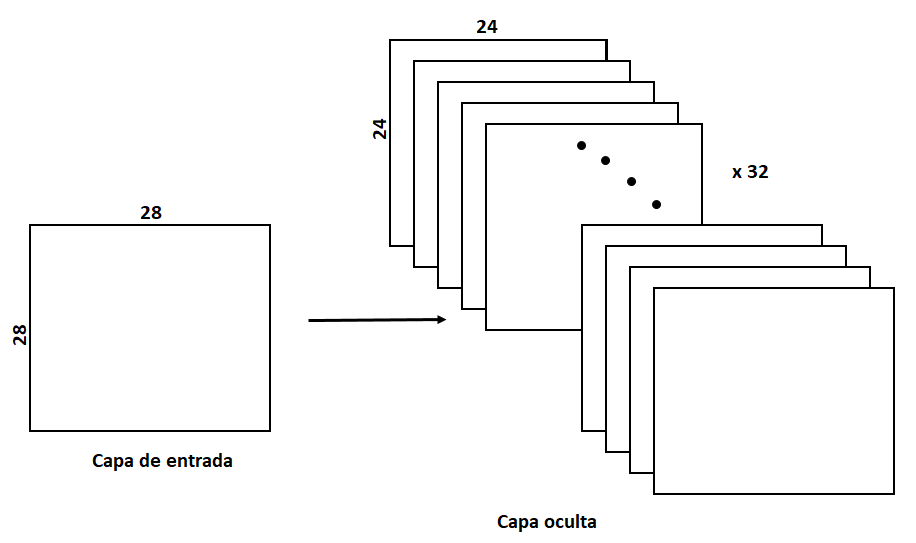
\includegraphics{imagenes/capitulo1/primera_capa_convolucional.png}

}

\caption{\label{fig-primera-capa-convolucional}Primera capa de la red
convolucional con 32 filtros}

\end{figure}

Al resultado de la aplicación de los diferentes filtros se les suele
aplicar la función de activación denominada RELU y que ya se comentó en
la introducción. Una interesante fuente de información es la
documentación del software gratuito GIMP donde expone diferentes efectos
que se producen en las imágenes al aplicar diversas convoluciones. Un
ejmplo claro y didáctico lo podemos obtener de la docuemntación del
software libre de dibujo y tratamiento de imágenes denominado GIMP
(https://docs.gimp.org/2.6/es/plug-in-convmatrix.html). Algunos de estos
efectos nos ayudan a entender la operación de los filtros en las redes
convolucionales y cómo afectan a las imágenes, en concreto, el ejemplo
que presenta lo realiza sobre la figura del Taj Mahal El filtro enfocar
lo que consigue es afinar los rasgos, los contornos lo que nos permite
agudizar los objetos de la imagen. Toma el valor central de la matriz de
cinco por cinco lo multiplica por cinco y le resta el valor de los
cuatro vecinos. Al final hace una media, lo que mejora la resolución del
pixel central porque elimina el ruido o perturbaciones que tiene de sus
pixeles vecinos. El filtro enfocar (Sharpen)

Lo contario al filtro enfocar lo obtenemos a través de la matriz
siguiente, difuminando la imagen al ser estos píxeles mezclados o
combinados con los pixeles cercanos. Promedia todos los píxeles vecinos
a un pixel dado lo que implica que se obtienen bordes borrosos. Filtro
desenfocar

Filtro Detectar bordes (Edge Detect) Este efecto se consigue mejorando
los límites o las aristas de la imagen. En cada píxel se elimina su
vecino inmediatamente anterior en horizontal y en vertical. Se eliminan
las similitudes vecinas y quedan los bordes resaltados. Al pixel central
se le suman los cuatro píxeles vecinos y lo que queda al final es una
medida de cómo de diferente es un píxel frente a sus vecinos. En el
ejemplo, al hacer esto da un valor de cero de ahí que se observen tantas
zonas oscuras.

Filtro Repujado (Emboss) En este filto se observa que la matriz es
simétrica y lo que intenta a través del diseño del filtro es mejorar los
píxeles centrales y de derecha abajo restándole los anteriores. Se
obtiene lo que en fotografía se conoce como un claro oscuro. Trata de
mejorar las partes que tienen mayor relevancia.

\hypertarget{pooling}{%
\subsection{Pooling}\label{pooling}}

Con la operación de pooling se trata de condensar la información de la
capa convolucional. A este procedimiento también se le conoce como
submuestreo. Es simplemente una operación en la que reducimos los
parámetros de la red. Se aplica normalmente a través de dos operaciones:
max-pooling y mean-pooling, que también es conocido como
average-pooling. Tal y como se observa en la imagen siguiente, desde la
capa de convolución se genera una nueva capa aplicando la operación a
todas las agrupaciones, donde previamente hemos elegido el tamaño de la
región; en la figura siguiente es de tamaño 2, con lo que pasamos de un
espacio de 24 x 24 neuronas a la mitad, 12 x 12 en la capa de pooling.

Figura 71. etapa de pooling de tamaño 2 x 2

\begin{figure}

{\centering 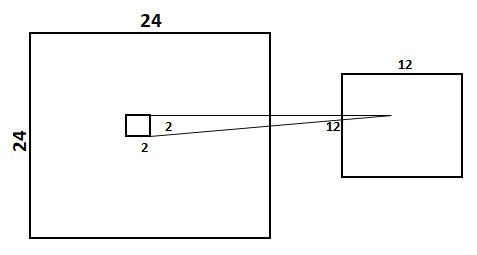
\includegraphics{imagenes/capitulo1/pooling.png}

}

\caption{\label{fig-pooling}etapa de pooling de tamaño 2 x 2}

\end{figure}

Vamos a estudiar el pooling suponiendo que tenemos una imagen de 5 x 5
píxeles y que queremos efectuar una agrupación max-pooling. Es la más
utilizada, ya que obtiene buenos resultados. Observamos los valores de
la matriz y se escoge el valor máximo de los cuatro bloques de matrices
de dos por dos. Max Pooling

En la agrupación Average Pooling la operación que se realiza es
sustituir los valores de cada grupo de entrada por su valor medio. Esta
transformación es menos utilizada que el max-pooling.

La transformación max-pooling presenta un tipo de invarianza local:
pequeños cambios en una región local no varían el resultado final
realizado con el max -- pooling: se mantiene la relación espacial. Para
ilustrar este concepto hemos escogido la imagen que presenta Torres
(2020) donde se ilustra como partiendo de una matriz de 12 x 12 que
representa al número 7, al aplicar la operación de max-pooling con una
ventana de 2 x 2 se conserva la relación espacial.

\begin{figure}

{\centering 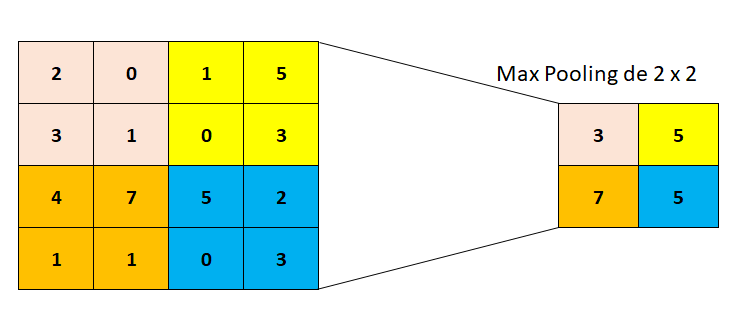
\includegraphics{imagenes/capitulo1/max_pooling.png}

}

\caption{\label{fig-max-pooling}Max Pooling}

\end{figure}

\begin{figure}

{\centering 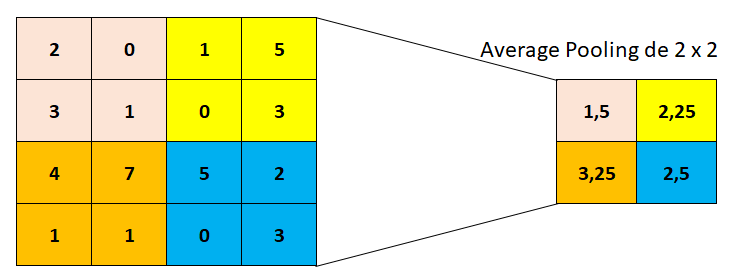
\includegraphics{imagenes/capitulo1/average_pooling.png}

}

\caption{\label{fig-average-pooling}Average Pooling}

\end{figure}

Fuente: Torres. J. (2020)

\hypertarget{padding}{%
\subsection{Padding}\label{padding}}

Para explicar el concepto del Padding vamos a suponer que tenemos una
imagen de 5 x 5 píxeles, es decir 25 neuronas en la capa de entrada, y
que elegimos, para realizar la convolución, una ventana de 3 x 3. El
número de neuronas de la capa oculta resultará ser de nueve. Enumeramos
los píxeles de la imagen de forma natural del 1 al 25 para que resulte
más sencillo de entender.

\begin{figure}

{\centering 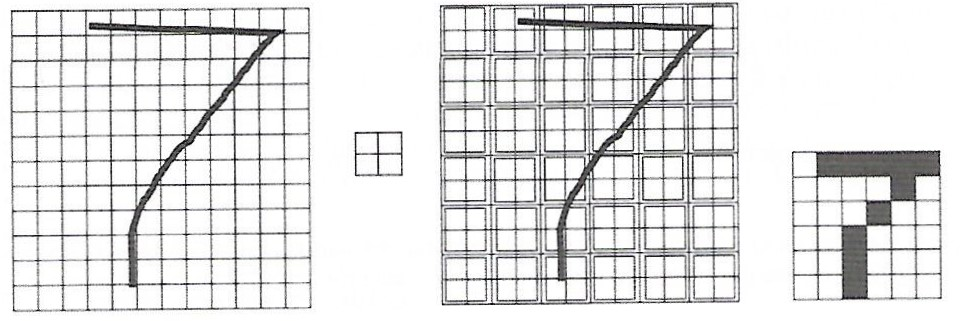
\includegraphics{imagenes/capitulo1/transformacion_pooling.png}

}

\caption{\label{fig-transformacion-pooling}mantenimiento del pooling con
la transformación}

\end{figure}

Pero si queremos obtener un tensor de salida que tenga las mismas
dimensiones que la entrada podemos rellenar la matriz de ceros antes de
deslizar la ventana por ella. Vemos la figura siguiente donde ya se ha
rellenado de valores cero y obtenemos, después de deslizar la ventana de
3 x3 de izquierda a derecha y de arriba abajo, las veinticinco matrices
de la figura nº 71

\begin{figure}

{\centering 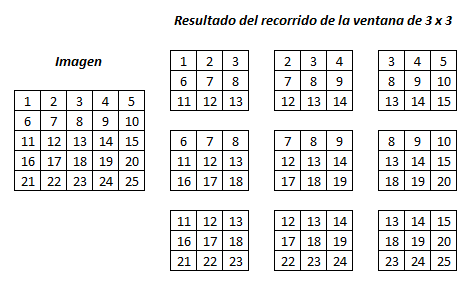
\includegraphics{imagenes/capitulo1/sin_padding.png}

}

\caption{\label{fig-sin-padding}Operación de convolución con una ventana
de 3 x 3}

\end{figure}

Figura nº 74. imagen con relleno de ceros

\begin{figure}

{\centering 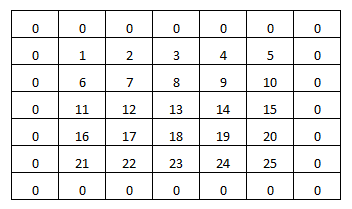
\includegraphics{imagenes/capitulo1/relleno_ceros.png}

}

\caption{\label{fig-relleno-ceros}Imagen con relleno de ceros}

\end{figure}

Cuando utilizamos el programa keras disponemos de dos opciones para
llevar a cabo esta operación de padding: ``same'' y ``valid''. Si
utilizamos ``valid'' implica no hacer padding y el método ``same''
obliga a que la salida tenga la misma dimensión que la entrada.

\begin{figure}

{\centering 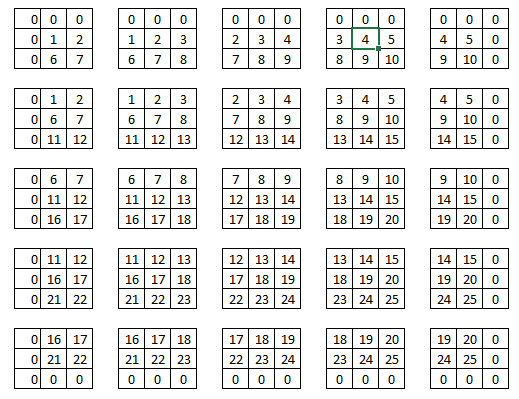
\includegraphics{imagenes/capitulo1/con_padding.png}

}

\caption{\label{fig-con-padding}Operación de convolución con ventana 3 x
3 y padding}

\end{figure}

\hypertarget{stride}{%
\subsection{Stride}\label{stride}}

Hasta ahora, la forma de recorrer la matriz a través de la ventana se
realiza desplazándola de un solo paso, pero podemos cambiar este
hiperparámetro conocido como stride. Al aumentar el paso se decrementa
la información que pasará a la capa posterior. A continuación, se
muestra el resultado de las cuatro matrices que obtenemos con un stride
de valor 3.

\begin{figure}

{\centering 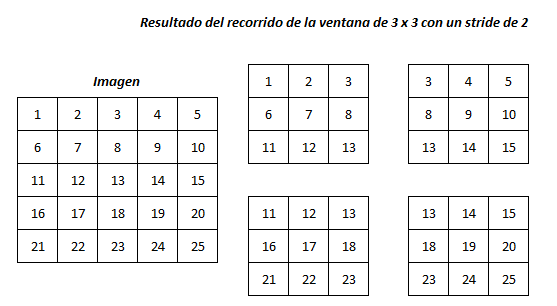
\includegraphics{imagenes/capitulo1/con_stride2.png}

}

\caption{\label{fig-con-stride2}Operación de convolución con una ventana
de 3 x 3 y stride 2}

\end{figure}

Finalmente, para resumir, una red convolucional contiene los siguientes
elementos: • Entrada: Son el número de pixeles de la imagen. Serán alto,
ancho y profundidad. Tenemos un solo color (escala de grises) o tres:
rojo, verde y azul. • Capa de convolución: procesará la salida de
neuronas que están conectadas en «regiones locales» de entrada (es decir
pixeles cercanos), calculando el producto escalar entre sus pesos (valor
de pixel) y una pequeña región a la que están conectados. En este
epígrafe se presentan las imágenes con 32 filtros, pero puede realizarse
con la cantidad que deseemos. • «Capa RELU» Se aplicará la función de
activación en los elementos de la matriz. • POOL (agrupar) o
Submuestreo: Se procede normalmente a una reducción en las dimensiones
alto y ancho, pero se mantiene la profundidad. • CAPA tradicional. Se
finalizará con la red de neuronas feedforward (Perceptrón multicapa que
se denomina normalmente como red densamente conectada) que vinculará con
la última capa de subsampling y finalizará con la cantidad de neuronas
que queremos clasificar. En el gráfico siguiente se muestran todas las
fases de una red neuronal convolucional.

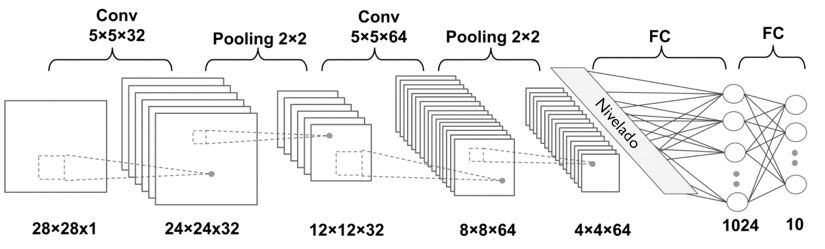
\includegraphics{imagenes/capitulo1/convolucion_completa.png} Fuente:
Raschka y Mirjalili (2019)

\hypertarget{redes-convolucionales-con-nombre-propio}{%
\subsection{Redes convolucionales con nombre
propio}\label{redes-convolucionales-con-nombre-propio}}

Existen en la actualidad muchas arquitecturas de redes neuronales
convolucionales que ya están preparadas, probadas, disponibles e
incorporadas en el software de muchos programas como Keras y Tensorflow.
Vamos a comentar algunos de estos modelos, bien por ser los primeros, o
por sus excelentes resultados en concursos como el ILSVRC (Large Scale
Visual Recognition Challenge). Estas estructuras merecen atención dado
que son excelentes para estudiarlas e incorporarlas por su notable
éxito. El ILSVRC fue un concurso celebrado de 2011 a 2016 de donde
nacieron las principales aportaciones efectuadas en las redes
convolucionales. Este concurso fue diseñado para estimular la innovación
en el campo de la visión computacional. Actualmente se desarrollan este
tipo de concursos a través de la plataforma web: https://www.kaggle.com/
Para ver más prototipos de redes convolucionales y los últimos avances y
consejos sobre las redes convolucionales se puede consultar el siguiente
artículo ``Recent Advances in Convolutional Neural Networks'' de
Jiuxiang. G. et al.~(2019) Los cinco modelos más destacados hasta el año
2017 son los siguientes: LeNet-5, Alexnet, GoogLeNet, VGG y Restnet. 1.
LeNet-5. Este modelo de Yann LeCun de los años 90 consiguió excelentes
resultados en la lectura de códigos postales consta de imágenes de
entrada de 32 x 32 píxeles seguida de dos etapas de convolución --
pooling, una capa densamente conectada y una capa softmax final que nos
permite conocer los números o las imágenes. 2. AlexNet. Fue la
arquitectura estrella a partir del año 2010 en el ILSVRC y popularizada
en el documento de 2012 de Alex Krizhevsky, et
al.~titulado''Clasificación de ImageNet con redes neuronales
convolucionales profundas''. Podemos resumir los aspectos clave de la
arquitectura relevantes en los modelos modernos de la siguiente manera:
• Empleo de la función de activación ReLU después de capas
convolucionales y softmax para la capa de salida. • Uso de la agrupación
máxima en lugar de la agrupación media. • Utilización de la
regularización de Dropout entre las capas totalmente conectadas. •
Patrón de capa convolucional alimentada directamente a otra capa
convolucional. • Uso del aumento de datos (Data Aumentation,) 3. VGG.
Este prototipo fue desarrollado por un grupo de investigación de
Geometría Visual en Oxford. Obtuvo el segundo puesto en la competición
del año 2014 del ILSVRC. Las aportaciones principales de la
investigación se pueden encontrar en el documento titulado ``~Redes
convolucionales muy profundas para el reconocimiento de imágenes a gran
escala~'' desarrollado por Karen Simonyan y Andrew Zisserman. Este
modelo contribuyó a demostrar que la profundidad de la red es una
componente crítica para alcanzar unos buenos resultados. Otra diferencia
importante con los modelos anteriores y que actualmente es muy utilizada
es el uso de un gran número de filtros y de tamaño reducido. Estas redes
emplean ejemplos de dos, tres e incluso cuatro capas convolucionales
apiladas antes de usar una capa de agrupación máxima. En esta
arquitectura el número de filtros aumenta con la profundidad del modelo.
El modelo comienza con 64 y aumenta a través de los filtros de 128, 256
y 512 al final de la parte de extracción de características del modelo.
Los investigadores evaluaron varias variantes de la arquitectura si bien
en los programas sólo se hace referencia a dos de ellas que son las que
aportan un mayor rendimiento y que son nombradas por las capas que
tienen: VGG-16 y VGG-19. 4. GoogLeNet. GoogLeNet fue desarrolado por
investigadores de Google Research. de Google, que con su módulo
denominado de inception reduce drásticamente los parámetros de la red
(10 veces menos que AlexNet) y de ella han derivado varias versiones
como la Inception-v4. Esta arquitectura ganó la competición en el año
2014 y su éxito se debió a que la red era mucho más profunda (muchas más
capas) y como ya se ha indicado introdujeron en el modelo las subredes
llamadas inception. Las aportaciones principales en el uso de capas
convolucionales fueron propuestos en el documento de 2015 por Christian
Szegedy, et al.~titulado ``~Profundizando con las convoluciones~''.
Estos autores introducen una arquitectura llamada ``inicio'' y un modelo
específico denominado GoogLenet. El módulo inicio es un bloque de capas
convolucionales paralelas con filtros de diferentes tamaños y una capa
de agrupación máxima de 3 × 3, cuyos resultados se concatenan. Otra
decisión de diseño fundamental en el modelo inicial fue la conexión de
la salida en diferentes puntos del modelo que lograron realizar con la
creación de pequeñas redes de salida desde la red principal y que fueron
entrenadas para hacer una predicción. La intención era proporcionar una
señal de error adicional de la tarea de clasificación en diferentes
puntos del modelo profundo para abordar el problema de los gradientes de
fuga. 5. Red Residual o ResNet. Esta arquitectura gano la competición de
2015 y fue creada por el grupo de investigación de Microsoft. Se puede
ampliar la información en He, et al.~en su documento de 2016 titulado
``~Aprendizaje profundo residual para el reconocimiento de la imagen~''.
Esta red es extremadamente profunda con 152 capas, confirmando al pasar
los años que las redes son cada vez más profundas, más capas, pero con
menos parámetros que estimar. La cuestión clave del diseño de esta red
es la incorporación de la idea de bloques residuales que hacen uso de
conexiones directa. Un bloque residual, según los autores, ``es un
patrón de dos capas convolucionales con activación ReLU donde la salida
del bloque se combina con la entrada al bloque, por ejemplo, la conexión
de acceso directo'' Otra clave, en este caso para el entrenamiento de la
red tan profunda es lo que llamaron skip connections que implica que la
señal con la que se alimenta una capa también se agregue a una capa que
se encuentre más adelante. Resumiendo, las tres principales aportaciones
de este modelo son: • Empleo de conexiones de acceso directo. •
Desarrollo y repetición de los bloques residuales. • Modelos muy
profundos (152 capas) Aunque se encuentran otros modelos que también son
muy populares con 34, 50 y 101 capas. Una buena parte de los modelos
comentados se incluyen en la librería de Keras y se pueden encontrar en
la siguiente dirección de internet: https://keras.io/api/applications/
Según los autores del programa Keras: ``Las aplicaciones Keras son
modelos de aprendizaje profundo que están disponibles junto con pesos
preentrenados. Estos modelos se pueden usar para predicción, extracción
de características y ajustes. Los pesos se descargan automáticamente
cuando se crea una instancia de un modelo. Se almacenan en
\textasciitilde{} / .keras / models /. Tras la creación de instancias,
los modelos se construirán de acuerdo con el formato de datos de imagen
establecido en su archivo de configuración de Keras en \textasciitilde{}
/ .keras / keras.json. Por ejemplo, si ha configurado
image\_data\_format = channel\_last, cualquier modelo cargado desde este
repositorio se construirá de acuerdo con la convención de formato de
datos TensorFlow,''Altura-Ancho-Profundidad''.

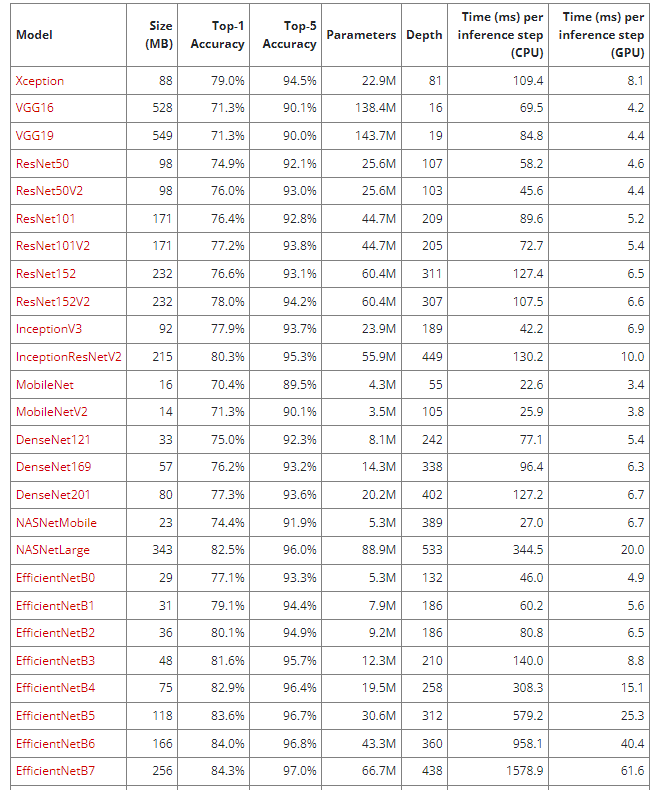
\includegraphics{imagenes/capitulo1/modelos_entrenados.png} Fuente :
https://keras.io/api/applications/

\hypertarget{redes-nueronales-recurrentes}{%
\section{Redes Nueronales
Recurrentes}\label{redes-nueronales-recurrentes}}

\hypertarget{autoencoders}{%
\section{Autoencoders}\label{autoencoders}}

\textbf{Bases del Autoencoder} Los Autoencoders (AE) son uno de los
tipos de redes neuronales que caen dentro del ámbito del Deep Learning,
en la que nos encontramos con un modelo de aprendizaje no supervisado.
Ya se empezó a hablar de AE en la década de los 80 (Bourlard and Kamp
1988), aunque es en estos últimos años donde más se está trabajando con
ellos. La arquitectura de un AE es una Red Neuronal Artificial (ANN por
sus siglas en inglés) que se encuentra dividida en dos partes, encoder y
decoder (Charte et al.~2018), (Goodfellow, Bengio, and Courville 2016).
El encoder va a ser la parte de la ANN que va codificar o comprimir los
datos de entrada, y el decoder será el encargado de regenerar de nuevo
los datos en la salida. Esta estructura de codificación y decodificación
le llevará a tener una estructura simétrica. El AE es entrenado para ser
capaz de reconstruir los datos de entrada en la capa de salida de la
ANN, implementando una serie de restricciones (la reducción de elementos
en las capas ocultas del encoder) que van a evitar que simplemente se
copie la entrada en la salida. Si recordamos la estructura de una ANN
clásica o también llamada Red Neuronal Densamente Conectada (ya que cada
neurona conecta con todas las de la siguiente capa) nos encontramos en
que en esta arquitectura, generalmente, el número de neuronas por capa
se va reduciendo hasta llegar a la capa de salida que debería ser
normalmente un número (si estamos en un problema regresión), un dato
binario (si es un problema de clasificación). Figura nº 86: Red Neuronal
Clasica

Fuente: Elaboración propia Si pensamos en una estructura básica de AE en
la que tenemos una capa de entrada, una capa oculta y una capa de
salida, ésta sería su representación:

Figura nº 87: Autoencoder básico

Fuente: Elaboración propia Donde los valores de son los datos de entrada
y los datos son la reconstrucción de los mismos después de pasar por la
capa oculta que tiene sólo dos dimensiones. El objetivo del
entrenamiento de un AE será que estos valores de sean lo más parecidos
posibles a los . Según (Charte et al.~2018) los AE se puden clasificar
según el tipo de arquitectura de red en: • Incompleto simple •
Incompleto profundo • Extra dimensionado simple • Extra dimensionado
profundo

Figura nº 88: Tipos de Autoencoders por arquitectura

Fuente: Elaboración propia Cuando hablamos de Incompleto nos referimos a
que tenemos una reducción de dimensiones que permite llegar a conseguir
una ``compresión'' de los datos iniciales como técnica para que aprenda
los patrones internos. En el caso de Extra dimensionado es cuando
subimos de dimensión para conseguir que aprenda esos patrones. En este
último caso sería necesario aplicar técnicas de regularización para
evitar que haya un sobreajuste en el aprendizaje. Cuando hablamos de
Simple estamos haciendo referencia a que hay una única capa oculta, y en
el caso de Profundo es que contamos con más de una capa oculta.
Normalmente se trabaja con las arquitecturas de tipo Incompleto
profundo, sobre todo cuando se está trabajando con tipos de datos que
son imágenes. Aunque también podríamos encontrar una combinación de
Incompleto con Extra dimensionado profundo cuando trabajamos con tipos
de datos que no son imágenes y así crecer en la primera o segunda capa
oculta, para luego reducir. Esto nos permitiría por ejemplo adaptarnos a
estructuras de AE en las que trabajemos con número de neuronas en una
capa que sean potencia de 2, y poder construir arquitecturas dinámicas
en función del tamaño de los datos, adaptándolos a un tamaño prefijado.
A continuación, vemos un gráfico de una estructura mixta Extra
dimensionado - Incompleto profundo. Figura nº 89: Autoencoder Mixto
(Incompleto y Extra dimensionado)

Fuente: Elaboración propia Idea intuitiva del uso de Autoencoders Si un
AE trata de reproducir los datos de entrada mediante un encoder y
decoder, ¿que nos puede aportar si ya tenemos los datos de entrada? Ya
hemos comentado que la red neuronal de un AE es simétrica y está formada
por un encoder y un decoder, además cuando trabajamos con los AE que son
incompletos, se está produciendo una reducción del tamaño de los datos
en la fase de codificación y de nuevo una regeneración a partir de esos
datos más pequeños al original. Ya tenemos uno de los conceptos más
importantes de los AE que es la reducción de dimensiones de los datos de
entrada. Estas nuevas variables que se generan una vez pasado el encoder
se les suele llamar el espacio lantente. Este concepto de reducción de
dimensiones en el mundo de la minería de datos lo podemos asimiliar
rápidamente a técnicas como el Análisis de Componentes Principales
(PCA), que nos permite trabajar con un número más reducido de
dimensiones que las originales. Igualmente, esa reducción de los datos y
la capacidad de poder reconstruir el original podemos asociarlo al
concepto de compresión de datos, de forma que con el encoder podemos
comprimir los datos y con el decoder los podemos descomprimir. En este
caso habría que tener en cuenta que sería una técnica de compresión de
datos con pérdida de información (JPG también es un formato de
compresión con pérdida de compresión). Es decir, con los datos
codificados y el AE (pesos de la red neuronal), seríamos capaces de
volver a regenerar los datos originales. Otra de las ideas alrededor de
los AE es que, si nosotros tenemos un conjunto de datos de la misma
naturaleza y los entrenamos con nuestro AE, somos capaces de construir
una red neuronal (pesos en la red neuronal) que es capaz de reproducir
esos datos a través del AE. Que ocurre si nosotros metemos un dato que
no era de la misma naturaleza que los que entrenaron el AE, lo que
tendremos entonces es que al recrear los datos originales no va a ser
posible que se parezca a los datos de entrada. De forma que el error que
vamos a tener va a ser mucho mayor por no ser datos de la misma
naturaleza. Esto nos puede llevar a construir un AE que permita detectar
anomalías, es decir, que seamos capaces de detectar cuando un dato es
una anomalía porque realmente el AE no consigue tener un error lo
bastante pequeño. Según lo visto de forma intuitiva vamos a tener el
encoder que será el encargado de codificar los datos de entrada y luego
tendremos el decoder que será el encargado de realizar la decodificación
y conseguir acercarnos al dato original . Es decir intentamos conseguir
. Si suponemos un Simple Autoencoder en el que tenemos una única capa
oculta, con una función de activación intermedia y una función de
activación de salida y los parámetros y represetan los parámetros de la
red neuronal en cada capa, tendríamos la siguiente expresión: {[}190{]}
{[}191{]}

Así tendremos que donde será la reconstrucción de Una vez tenemos la
idea intuitiva de para qué nos puede ayudar un AE, recopilamos algunos
de los principales usos sobre los que actualmente se está trabajando.
Más adelante ,comentaremos algunos de ellos con más detalle. Principales
Usos de los Autoencoders A continuación, veamos la explicación de cuales
son algunos de los principales usos de los autoencoders: Reducción de
dimensiones / Compresión de datos En la idea intuitiva de los AE ya
hemos visto claro que se pueden usar para la reducción de dimensiones de
los datos de entrada. Si estamos ante unos datos de entrada de tipo
estructurado estamos en un caso de reducción de dimensiones clásico, en
el que queremos disminuir el número de variables con las que trabajar.
Muchas veces este tipo de trabajo se hace mediante el PCA (Análisis de
Componente Principales, por sus siglas en inglés), sabiendo que lo que
se realiza es una transformación lineal de los datos, ya que conseguimos
unas nuevas variables que son una combinación lineal de las mismas. En
el caso de los AE conseguimos mediante las funciones de activación no
lineales (simgmoide, ReLu, tanh, etc) combinaciones no lineales de las
variables originales para reducir las dimensiones. También existen
versiones de PCA no lineales llamadas Kernel PCA que mediante las
técnicas de kernel son capaces de construir relaciones no lineales. En
esta línea estamos viendo que cuando el encoder ha actuado, tenemos unos
nuevos datos más reducidos y que somos capaces de practicamente volver a
reproducir teniendo el decoder. Podríamos pensar en este tipo de técnica
para simplemente comprimir información. Hay que tener en cuenta que este
tipo de técnicas no se pueden aplicar a cualquier dato que queramos
comprimir, ya que debemos haber entrenado al AE con unos datos de
entrenamiento que ha sido capaz de obtener ciertos patrones de ellos, y
por eso es capaz luego de reproducirlos. Búsqueda de imágenes Cuando
pensamos en un buscador de imágenes nos podemos hacer a la idea que el
buscar al igual que con el texto nos va a mostrar entradas que seán
imágenes parecidas a la que estamos buscando. Si construimos un
autoencoder, el encoder nos va a dar unas variables con información para
poder recrear de nuevo la imagen. Lo que parece claro es que si hay muy
poca distancia entre estas variables y otras la reconstrucción de la
imagen será muy parecida. Así nosotros podemos entrenar el AE con
nuestro conjunto de imágenes, una vez tenemos el AE pasamos el encoder a
todas las imágenes y las tenemos todas en ese nuevo espacio de
variables. Cuando queremos buscar una imagen, le pasamos el autoencoder,
y ya buscamos las más cercanas a nuestra imagen en el espacio de
variables generado por el encoder. Detección de Anomalías Cuando estamos
ante un problema de clasificación y tenemos un conjunto de datos que
está muy desbalanceado, es decir, tenemos una clase mayoritaria que es
mucho más grande que la minoritaria (posiblemente del orden de más del
95\%), muchas veces es complicado conseguir un conjunto de datos
balanceado que sea realmente bueno para hacer las predicciones. Cuando
estamos en estos entornos tan desbalanceados muchas veces se dice que
estamos ante un sistema para detectar anomalías. Un AE nos puede ayudar
a detectar estas anomalías de la siguiente forma: • Tomamos todos los
datos de entrenamiento de la clase mayoritaria (o normales) y
construimos un AE para ser capaces de reproducirlos. Al ser todos estos
datos de la misma naturaleza conseguiremos entrenar el AE con un error
muy pequeño. • Ahora tomamos los datos de la clase minoritaria (o a
nomalías) y los pasamos a través del AE obteniendo unos errores de
reconstrucción. • Definimos el umbral de error que nos separará los
datos normales de las anomalías, ya que el AE sólo está entrenado con
los normales y conseguirá un error más alto con las anomalías al
reconstruirlas. • Cogemos los datos de test y los vamos pasando por el
AE, si el error es menor del umbral, entonces será de la clase
mayoritaria. Si el error es mayor que el umbral, entonces estaremos ante
una anomalía. Eliminación de ruido Otra de las formas de uso de los
autoencoders en tratamiento de imágenes es para eliminar ruido de las
mismas, es decir poder quitar manchas de las imágenes. La forma de hacer
esto es la siguiente: • Partimos de un conjunto de datos de
entrenamiento (imágenes) a las que le metemos ruido, por ejemplo,
modificando los valores de cada pixel usando una distribución normal, de
forma que obtenemos unos datos de entrenamiento con ruido. • Construimos
el AE de forma que los datos de entrada son los que tienen ruido, pero
los de salida vamos a forzar que sean los originales. De forma que
intentamos que aprendan a reconstruirse como los que no tienen ruido. •
Una vez que tenemos el AE y le pasamos datos de test con ruido, seremos
capaces de reconstruirlos sin el ruido. Modelos generativos Cuando
hablamos de modelos generativos, nos referimos a AE que son capaces de
generar cosas nuevas a las que existían. De forma que mediante técnicas
como los Variational Autoencoders, los Adversarial Autoencoders seremos
capaces de generar nuevas imágenes que no teníamos inicialmente. Es
decir, podríamos pensar en poder tener un AE que sea capaz de
reconstruir imágenes de caras, pero que además con toda la información
aprendida fuera capaz de generar nuevas caras que realmente no existen.
Diseño del modelo de AE Transformación de datos Cuando se trabaja con
redes neuronales y en particular con AEs, necesitamos representar los
valores de las variables de entrada en forma numérica. En una red
neuronal todos los datos son siempre numéricos. Esto significa que todas
aquellas variables que sean categóricas necesitamos convertirlas en
numéricas. Además es muy conveniente normalizar los datos para poder
trabajar con valores entre 0 y 1, que van a ayudar a que sea más fácil
que se pueda converger a la solución. Como ya sabemos normalmente nos
encontramos que en una red neuronal las variables de salida son: • un
número (regresión) • una serie de números (regresión múltiple) • un dato
binario (clasificación binaria) • un número que representa una categoría
(clasifiación múltiple) En el caso de los AE puede que tengamos una gran
parte de las veces valores de series de números, ya que necesitamos
volver a representar los datos de entrada. Esto significa que tendremos
que conseguir en la capa de salida esos datos numéricos que teníamos
inicialmente, como si se tuviera una regresión múltiple. Arquitectura de
red Como ya se ha comentado en las redes neuronales, algunos de los
hiperparámetros más importantes en un AE son los relacionados con la
arquitectura de la red neuronal. Para la construcción de un AE vamos a
elegir una topología simétrica del encoder y el decoder. Durante el
diseño del AE necesitaremos ir probando y adaptando todos estos
hiperparámetros de la ANN para conseguir que sea lo más eficiente
posible: • Número de capas ocultas y neuronas en cada una • Función de
coste y pérdida • Optimizador • Función de activación en capas ocultas •
Función de activación en salida Número de capas ocultas y neuronas en
cada una La selección del número de capas ocultas y la cantidad de
neuronas en cada una va a ser un procedimiento de prueba y error en el
que se pueden probar muchas combinaciones. Es cierto que en el caso de
trabajar con imágenes y CNN ya hay muchas arquitecturas definidas y
probadas que consiguen muy buenos resultados. Por otro lado para tipos
de datos estructurados será muy dependiente de esos datos, de forma que
será necesario realizar diferentes pruebas para conseguir un buen
resultado. Función de coste y pérdida En este caso no hay ninguna
recomendación especial para las funciones de costes/pérdida y dependerá
al igual que en las redes neuronales de la naturaleza de los datos de
salida con los que vamos a trabajar. Optimizador Se recomienda usar el
optimizador ADAM (Diederik P. Kingma 2017) que es el que mejores
resultados ha dado en las pruebas según (Walia 2017), consiguiendo una
convergencia más rápida que con el resto de optimizadores.

Función de activación en capas ocultas En un AE las funciones de
activación en las capas ocultas van a conseguir establecer las
restricciones no lineales al pasar de una capa a la siguiente,
normalmente se evita usar la función de activación lineal en las capas
intermedias ya que queremos conseguir transformaciones no lineales. Se
recomienda usar la función de activación ReLu en las capas ocultas, ya
que parece ser que es la que mejores resultados da en la convergencia de
la solución y además menor coste computacional tiene a la hora de
realizar los cálculos. Función de activación en salida En la capa de
salida tenemos que tener en cuenta cual es el tipo de datos final que
queremos obtener, que en el caso de un AE es el mismo que el tipo de
dato de entrada. Normalmente las funciones de activación que se usarán
en la última capa seran: • Lineal con multiples unidades, para regresión
de varios datos numéricos • Sigmoid para valores entre 0 y 1 Tipos de
Autoencoders Una vez entendido el funcionamiento de los AE, veamos
algunos de los AE que se pueden construir para diversas tareas. • Simple
• Multicapa o Profundo • Sparse • Convolucional • Denoising •
Variational En la descripción de los tipos de AE vamos usar código en R
y en python y el framework keras con el backend Tensorflow. Todo el
código se proporciona aparte. Usaremos como dataset a MINIST, que
contiene 60.000/10.000 (entrenamiento/validación) imágenes de los
números del 0 al 9, escritos a mano. Cada imagen tiene un tamaño de
28x28 = 784 pixels, en escala de grises, con lo que para cada pixel
tendremos un valor entre 0 y 255 para definir cuál es su intensidad de
gris. Autoencoder Simple Vamos a describir como construir un autoencoder
Simple usando una red neuronal densamente conectada en lugar de usar una
red neuronal convolucional, para que sea más sencillo comprender el
ejemplo. Es decir, vamos a tratar los datos de entrada como si fueran
unos datos numéricos que queremos reproducir y no vamos a utilizar
ninguna de las técnicas asociadas a las redes convolucionales. Hay que
recordar que las redes convolucionales permiten mediante un tratamiento
de las imágenes (convolución, pooling, etc) conseguir mejores resultados
que si lo hiciéramos directamente con redes densamente conectadas. En
este caso tendremos una capa de entrada con 784 neuronas
(correspondientes a los pixels de cada imagen), una capa intermedia de
32 neuronas, y una capa de salida de nuevo de las 784 neuronas para
poder volver a obtener de nuevo los datos originales. En nuestro ejemplo
vamos a tener los siguientes elementos. • 1 capa de entrada (784 datos),
1 capa oculta (32 datos) y una capa de salida (784 datos) • La función
de coste/pérdida va a ser la Entropía • Usaremos el optimizador Adam •
Como función activación intermedia usaremos ReLu • Como función
activación de salida sigmoid (ya que queremos un valor entre 0 y 1 )
Autoencoder Sparse Ya hemos comentado que una forma de conseguir que un
autoencoder aprenda estructuras o correlaciones es la reducción del
número de neuronas, pero parte de este trabajo también se puede
conseguir mediante técnicas de sparsing (escasez). Este tipo de técnicas
se usan normalmente en las ANN para evitar el sobreajuste de nuestro
modelo, de forma que en cada actualización de los pesos de la red no se
tienen en cuenta todas las neuronas de la capa. Es decir, vamos a
conseguir que en las capas que decidamos no todas las neuronas van a
estar activadas, de esta manera además de ayudar a evitar el
sobreajuste, también conseguiremos crear esas correlaciones que ayudan a
construir el autoencoder. Existen dos metodos básicos para generar el
sparse que son: • Regularización L1 • Regularización L2 Básicamente los
dos métodos tratan de hacer que los pesos de las neuronas tengan valores
muy pequeños consiguiendo una distribución de pesos más regular. Esto lo
consiguen al añadir a la función de pérdida un coste asociado a tener
pesos grandes en las neuronas. Este peso se puede construir o bien con
la norma L1 (proporcional al valor absoluto) o con la norma L2
(proporcional al cuadrado de los coeficientes de los pesos). Básicamente
trabajaremos con un AE Simple, con una red densamente conectada, al que
le aplicaremos la regularización en su capa oculta. En nuestro ejemplo
vamos a tener los siguientes elementos. - 1 capa de entrada, 1 capaa
oculta y una capa de salida - Las capas ocultas tendrán aplicada la
Regularización L2 - La función de coste/pérdida va a ser la Entropía -
Usaremos el optimizador Adam - Como función activación intermedia
usaremos ReLu - Como función activación de salida sigmoid (ya que
queremos un valor entre 0 y 1) Autoencoder Multicapa o profundo Vamos a
pasar ahora a una versión del autoencoder donde habilitamos más capas
ocultas y hacemos que el descenso del número de neuronas sea más gradual
hasta llegar a nuestro valor deseado, para luego volver a reconstruirlo.
En este caso seguimos con redes densamente conectadas y aplicamos varias
capas intermedias reduciendo el número de neuronas en cada una hasta
llegar a la capa donde acaba el encoder para volver a ir creciendo en
las sucesivas capas hasta llegar a la de salida. En nuestro ejemplo
vamos a tener los siguientes elementos. - 1 capa de entrada (784 datos),
5 capa ocultas (32 datos intermedia) y una capa de salida (784 datos) -
La función de coste/pérdida va a ser la Entropía - Usaremos el
optimizador Adam - Como función activación intermedia usaremos ReLu -
Como función activación de salida sigmoid (ya que queremos un valor
entre 0 y 1) Autoencoder Convolucional En nuestro ejemplo al estar
trabajando con imágenes podemos pasar a trabajar con Redes
Convolucionales (CNN) de forma que en lugar de usar las capas densamente
conectadas que hemos usado hasta ahora, vamos a pasar a usar las
capacidades de las redes convolucionales. Al trabajar con redes
convolucionales necesitaremos trabajar con capas de convolución o
pooling para llegar a la capa donde acaba el encoder para volver a ir
creciendo aplicando operaciones de convolución y upsampling (contrario
al pooling). En nuestro ejemplo vamos a tener los siguientes elementos.
- 1 capa de entrada, 5 capas ocultas y una capa de salida - La función
de coste/pérdida va a ser la Entropía - Usaremos el optimizador Adam -
Como función activación intermedia usaremos ReLu - Como función
activación de salida sigmoid (ya que queremos un valor entre 0 y 1)
Autoencoder Denoising Vamos a usar ahora un autoencoder para hacer
limpieza en imagen, es decir, conseguir a partir de una imagen que tiene
ruido otra imagen sin ese ruido. Entrenaremos al autoencoder para que
limpie ``ruido'' que hay en la imagen y lo reconstruya sin ello. El
ruido lo vamos a generar mediante una distribución normal y
modificaremos el valor de los pixels de las imágenes. Usaremos estas
imágenes con ruido para que sea capaz de reconstruir la imagen original
sin ruido con el AE. Para realizar este proceso lo que haremos será\_ •
Crear nuevas imágenes con ruido • Entrenar el autoencoder con estas
nuevas imágenes • Calcular el error de reconstrucción respecto a las
imágenes originales Al estar trabajando con imágenes vamos a partir del
Autoencoder de Convolución para poder aplicar el denosing. En nuestro
ejemplo vamos a tener los siguientes elementos. - 1 capa de entrada, 5
capas ocultas y una capa de salida - La función de coste/pérdida va a
ser la Entropía - Usaremos el optimizador Adam - Como función activación
intermedia usaremos ReLu - Como función activación de salida sigmoid (ya
que queremos un valor entre 0 y 1) Autoencoder Variational Los
Variational Autoencoder son un tipo de modelo que se denomina
generativo, ya que va a permitir construir nuevas imágenes que no
existían a partir de otras imagenes con las que se ha entrenado a la red
neuronal. En realidad, es un autoencoder que durante el entrenamiento se
le regulariza para evitar un sobreajuste y asegurar que en el espacio
latente (intermedio) tenga buenas propiedades que permitan un buen
proceso generativo. El proceso de construir este tipo de AE es muy
parecido a los que ya hemos visto, con una pequeña diferencia en el paso
entre el proceso de encoder y el posterior decoder. Hasta ahora lo que
teníamos era que lo que obteníamos del encoder se lo pasábamos
directamente al decoder, en este caso, el resultado del encoder no va a
ser realmente un dato, sino una distribución de datos. De forma que al
decoder no se le pasa directamente lo que ha salido del encoder, si no
otro elemento cogido de la distribución generada. En este caso el
proceso sería: • Se codifica la entrada con el encoder no como un dato
concreto, sino como una distribución normal (media y desviación) • Se
toma una muestra de un punto del espacio latente a partir de la
distribución • Se decodifica el punto de muestra con el decoder • Se
calcula la función de pérdida con el error de reconstrucción y la parte
de regularización • Se usa el backpropagation a través de la red
neuronal para ajustar los pesos Figura nº 90: Autoencoder Mixto
(Incompleto y Extra dimensionado)

Fuente:
https://towardsdatascience.com/understanding-variational-autoencoders-vaes-f70510919f73
Una vez que tenemos entrenado nuestro autoencoder seremos capaces de
construir nuevas imágenes partiendo de puntos que estén en la
distribución del espacio latente, de forma que esas pequeñas variaciones
van a dar lugar a imágenes finales diferentes.

\hypertarget{arquiecturas-preentranadas}{%
\section{Arquiecturas Preentranadas}\label{arquiecturas-preentranadas}}

\hypertarget{detecciuxf3n-de-objetos}{%
\subsection{Detección de objetos}\label{detecciuxf3n-de-objetos}}

\hypertarget{tratamiento-de-audios}{%
\subsection{Tratamiento de audios}\label{tratamiento-de-audios}}

\hypertarget{tareas-sobre-textos}{%
\subsection{Tareas sobre textos}\label{tareas-sobre-textos}}

\hypertarget{aprendizaje-por-refuerzo}{%
\section{Aprendizaje por Refuerzo}\label{aprendizaje-por-refuerzo}}

\hypertarget{introducciuxf3n-3}{%
\subsection{Introducción}\label{introducciuxf3n-3}}

Hasta ahora hemos visto como el Deep Learning se usa para el
\textbf{aprendizaje supervisado} y el \textbf{aprendizaje no
supervisado}, pero vamos a dar un paso más, en el que veremos como usar
Deep Learning en otro tipo de aprendizaje llamado \textbf{aprendizaje
por refuerzo}.

El \textbf{Aprendizaje por Refuerzo} (\textbf{RL} por sus siglas en
ingles, Reinforcement Learning) trata de conseguir que el sistema
aprenda mediante recompensa/castigo, en función de si los pasos que da
son buenos o malos. De esta manera, cuanta mayor recompensa se tenga es
que nuestro sistema se ha acercado a la solución buena. Se trata de
aprender mediante la interacción y la retroalimentación de lo que
ocurra.

Partiremos de dos elementos clave \textbf{agente} (es el que aprende y
toma decisiones), y el \textbf{entorno} (donde el agente aprende y
decide que acciones tomar). Tendremos que el agente podrá realizar
\textbf{acciones} que normalmente provocarán un cambio de
\textbf{estado} y a la vez se tendrá una \textbf{recompensa} (positiva o
negativa) en función de la acción tomada en el entorno en ese momento.

Es decir, nos encontraremos un agente que realizará una acción \(a_t\)
en el tiempo \(t\), esta acción afectará al entorno que estará en un
estado \(S_t\) y mediante esta acción cambiará a un estado \(S_{t+1}\) y
además dará una recompensa \(r_{t+1}\) en función de los malo o bueno
que haya sido este paso.

El agente volverá a examinar el nuevo estado del entorno \(S_{t+1}\) y
la nueva recompensa recibida \(r_{t+1}\) y volverá a tomar la decisión
de realizar una nueva acción \(a_{t+1}\).

\begin{figure}

{\centering 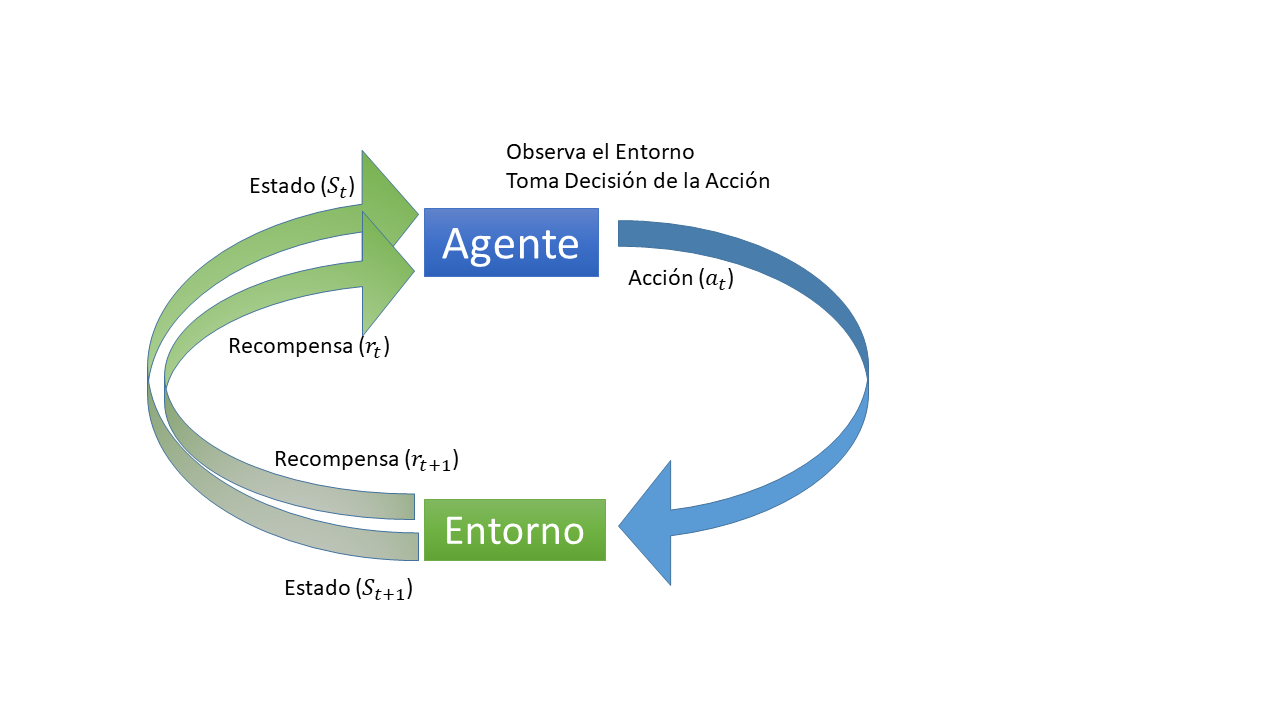
\includegraphics[width=1\textwidth,height=\textheight]{imagenes/reinforcement_learning/rl-diagrama.png}

}

\caption{Esquema Aprendizaje por Refuerzo - Fuente: Propia}

\end{figure}

\hypertarget{historia-del-aprendizaje-por-refuerzo}{%
\subsection{Historia del Aprendizaje por
Refuerzo}\label{historia-del-aprendizaje-por-refuerzo}}

\hypertarget{formalismo-matemuxe1tico}{%
\subsection{Formalismo Matemático}\label{formalismo-matemuxe1tico}}

El formalismo matemático para el Aprendizaje por Refuerzo está basado en
los \textbf{Procesos de Decisión de Markov} (MDP por sus siglas en
ingles). (CS229 Lecture notes).

\hypertarget{propiedad-de-markov}{%
\subsubsection{Propiedad de Markov}\label{propiedad-de-markov}}

Si tenemos una secuencia de estados \(s_1, s_2, ..., s_t\) y tenemos la
probabilidad de pasar a otro estado \(s_{t+1}\), diremos que se cumple
la \textbf{Propiedad de Markov} si el \textbf{futuro} es independiente
del \textbf{pasado} y sólo se ve afectado por el \textbf{presente}, es
decir:

\[
\mathbb P[S_{t+1}| S_t] = \mathbb P[ S_{t+1}| S_t, s_{t-1}, ... S_2, S_1]
\]

Tendremos una \textbf{Matriz de Probabilidades de Transición} a una
matriz con las probabilidades de todos los posibles cambios de estado
que se puedan producir,
\[\mathcal P_{ss'}=\mathbb P[S_{t+1}=s'|S_t = s]\]

\hypertarget{proceso-de-markov}{%
\subsubsection{Proceso de Markov}\label{proceso-de-markov}}

Así llamaremos \textbf{Proceso de Markov} a un proceso aleatorio sin
memmoria, es decir, una secuencia de estados \(S_1, S_2, …\) con la
propiedad de Markov.

Un Proceso de Markov está formado por una dupla
\(<\mathcal S,\mathcal P>\),:

\begin{itemize}
\tightlist
\item
  \(\mathcal S\) conjunto finito de Estados
\item
  \(\mathcal P\) matriz de probabilidades de transición
\end{itemize}

\hypertarget{proceso-de-recompensa-de-markov}{%
\subsubsection{Proceso de Recompensa de
Markov}\label{proceso-de-recompensa-de-markov}}

LLamaremos \textbf{Proceso de Recompensa de Markov} (\textbf{MRP,} por
sus siglas en ingles) a una cuádrupla
\(<\mathcal S,\mathcal P,\mathcal R,\gamma>\), formada por:

\begin{itemize}
\tightlist
\item
  \(\mathcal S\) conjunto finito de Estados
\item
  \(\mathcal P\) matriz de probabilidades de transición
\item
  \(\mathcal R\) Función de recompensa definida como:
  \(\mathcal R_s=E[R_{t+1}|S_t=s]\), donde \(R_{t+1}\)es la recompensa
  obtenida de pasar al estado \(S_{t+1}\) desde el estado \(S_t\)
\item
  \(\gamma\) Factor de descuento, con \(\gamma \in [0,1]\)
\end{itemize}

En este contexto llamaremos \textbf{Saldo (}\(G_t\)\textbf{)} a la suma
de todas las recompensas conseguidas a partir del estado \(s_t\) con el
factor de descuento aplicado.

\[
G_t = R_{t+1} + \gamma R_{t+2} + \gamma^2 R_{t+3} + ... = \sum_{k=0}^\infty\gamma^kR_{t+k+1}
\]

El hecho de usar \(\gamma\) (\textbf{factor descuento}), nos permite dar
grandes recompensas lo antes posible, y no dar tanto valor a futuras
recompensas lejanas. También puede haber otras interpretaciones por
ejemplo a nivel económico, si la recompensa está basado en un dato
monetario real, tendría sentido que el dinero a futuro tendría menos
valor. También nos permite asegurar que este valor de \(G_t\) es finito
ya que produce que la serie sea convergente.

Cuando los valores del factor descuento se acercan a \textbf{0}
podríamos decir que nos fijamos sólo en los valores más cercanos de la
recompensa. En cambio cuando los valores se acercan a \textbf{1}
entonces les daremos más peso a los valores más lejanos de la
recompensa.

Una vez definido el Saldo podemos definir la \textbf{Función Valor de
Estado} como la función que nos da el \textbf{Saldo Esperado} comenzando
por el estado \(s\). Es decir:

\[
V(s) = \mathbb E[G_t|S_t=s]
\]

Esta función nos dice cómo de bueno es partir de este estado y
continuar.

\hypertarget{proceso-de-decisiuxf3n-de-markov}{%
\subsubsection{Proceso de Decisión de
Markov}\label{proceso-de-decisiuxf3n-de-markov}}

Un \textbf{Proceso de Decisión de Markov (MDP por sus siglas en inglés)}
es un tupla \(<\mathcal S,\mathcal A,\mathcal P,\mathcal R, \gamma >\)
donde:

\begin{itemize}
\item
  \(\mathcal S\) es el conjunto de posibles \textbf{estados}.
\item
  \(\mathcal A\) es el conjunto de posibles \textbf{acciones}.
\item
  \(\mathcal P\) son las \textbf{probabilidades de transición} de un
  estado a otro en función de la acción realizada. Por cada estado y
  acción hay una distribución de probabilidad para pasar a otro estado.

  \[
  \mathcal P_{ss'}^a=\mathbb P[S_{t+1}=s'|S_t=s,A_t=a]\]
\item
  \(\gamma\) es el conocido como \textbf{factor de descuento} y tendrá
  un valor entre \([0,1)]\) y nos proporciona cuanto descontamos en las
  recompensas a futuro.
\item
  \(\mathcal R\) es la \textbf{Función de recompensa} definida como:
  \(\mathcal R_s^a=E[R\_{t+1}|S_t=s, A_t=a]\), donde \(R\_{t+1}\)es la
  recompensa obtenida de pasar al estado \(S_{t+1}\) desde el estado
\end{itemize}

Además tenemos que este \textbf{proceso estocástico} cumple la
\textbf{propiedad de Markov} que dice que el futuro es independiente del
pasado dado el presente. En términos de nuestro problema, podría decir
que pasar de un estado \(s_t\) al siguiente \(s_{t+1}\) sólo depende de
\(s_t\) y no de los anteriores estados \[
\mathbb P(s_{t+1}|s_t)= \mathbb P(s_{t+1}|s_1,s_2,...,s_t)
\]

Veamos cual es la \textbf{dinámica} de un MDP:

\begin{itemize}
\tightlist
\item
  Empezamos con un estado \(s_0 \in \mathcal S\)
\item
  Elegimos una acción \(a_0 \in \mathcal A\) (la política será la que la
  elija)
\item
  Obtenemos una recompensa \(R_1 = R(s_0) = R(s_0, a_0)\)
\item
  Elegimos una acción \(a_1 \in \mathcal A\)(la política será la que la
  elija)
\item
  Se transiciona aleatoriamente a un estado \(s_1\) en un función del
  valor de \(P_{s_0s_1}^{a_1}\)
\item
  Obtenemos una recompensa \(R_2 = R(s_1) = R(s_1, a_1)\)
\item
  Se transiciona a aleatoriamente a un estado \(s_12\) en un función del
  valor de \(P_{s_1s_2}^{a_2}\)
\item
  \ldots{}
\item
  Repetimos de forma iterativa este proceso
\end{itemize}

La meta en RL es elegir las \textbf{acciones} adecuadas en el tiempo
para \textbf{maximizar}:
\[\mathbb E[G_t] =\mathbb E[R(s_0) + \gamma R(s_1) + \gamma^2 R(s_2) + \gamma^3 R(s_3) + ...]\]
Que es conocido como la \textbf{hipotesis de la recompensa}.

Vamos a introducir el término de \textbf{política} como una función
\(\pi : \mathcal S \rightarrow \mathcal A\) que mapea los estados a las
acciones. Es decir, es la que decide que \textbf{acción} hay que
\textbf{ejecutar} en función de \textbf{cual} es el \textbf{estado} en
el que estamos. Una política podría ser determinística o estocástica. \[
a = \pi(s) \\
a = \pi (a|s)=\mathbb P[A=a|S=s]
\]

Una política define cual va a ser el comportamiento de un
\textbf{agente}. En un MDP las políticas dependen del estado actual, y
no de la historia de los estados pasados.

Diremos que estamos \textbf{ejecutando una política} \(\pi\) si cuando
estamos en un estado \(s\) aplicamos la acción \(a=\pi(s)\)

Definiremos:

\[
\mathcal P_{s,s`}^\pi = \sum_{a \in \mathcal A}\pi(a|s)\mathcal P_{s,s`}^a \\
\mathcal R_{s}^\pi = \sum_{a \in \mathcal A}\pi(a|s)\mathcal R_{s}^a 
\]

También definiremos la \textbf{Función Valor de Estado} para una
\textbf{política} \(\pi\) a la función que nos predice la recompensa a
futuro (el \textbf{saldo esperado}):
\[V^{\pi}(s)=\mathbb E_\pi[G_t|S_t=s]=
\mathbb E_\pi[R(s_t) + \gamma R(s_{t+1}) + \gamma^2 R(s_{t+2}) + \gamma^3 R(s_{t+3}) + ...|s_t=s]\]
Es decir, la esperanza de la suma de las recompensas con factor
descuento suponiendo el comienzo en \(s_t=s\) y tomando las acciones
bajo la política \(\pi\). Nos permite decir cómo de buenos o malos son
los estados.

Añadiremos el concepto de la \textbf{Función Valor de Acción,} también
llamada \textbf{Función de Calidad} (por eso se usa la \(Q\)
(Quality)\textbf{,} para una \textbf{política} \(\pi\) a la función que
nos predice la recompensa a futuro (el saldo esperado), suponiendo que
se se \textbf{parte de una acción} \(a\). \[
Q^\pi(s,a)=\mathbb E_\pi[G_t|S_t=s,A_t=a]\\
=\mathbb E_\pi[R(s_t) + \gamma R(s_{t+1}) + \gamma^2 R(s_{t+2}) + \gamma^3 R(s_{t+3}) + ...|s_t=s,A_t=a]
\] La función de \textbf{Valor de Estado} puede ser descompuesta en la
\textbf{recompensa inmediata} y el resto de la recompensa: \[
V^\pi(s) = \mathbb E_\pi[R_{t+1}+\gamma V^\pi(S_{t+1)}|S_t=s]
\] y del mismo modo se puede descomponer la función \textbf{Valor de
Acción}: \[
Q^\pi(s,a) = \mathbb E_\pi[R_{t+1}+\gamma Q^\pi(S_{t+1}, A_{t+1})|S_t=s,A_t=a]
\] Luego tenemos \[
V^\pi(s) = \sum_{a\in A}\pi(a|s)Q^\pi(s,a)
\]

y \[
Q^\pi(s,a) = R_s^a+\gamma \sum_{s'\in S} P_{ss'}^{a}V^\pi(s')
\]

Llegando a

\[
V^\pi(s) = \sum_{a\in A}\pi(a|s)(R_s^a+\gamma \sum_{s'\in S} P_{ss'}^{a}V^\pi(s'))
\]

y

\[
Q^\pi(s,a) = R_s^a+\gamma \sum_{s'\in S} P_{ss'}^{a}\sum_{a \in \mathcal A} \pi (a|s)Q^\pi(s',a)
\]

Dada una política \(\pi\) su \textbf{función valor de estado} asociada
\(V^{\pi}(s)\) cumple la \textbf{Ecuación de Bellman}:
\[V^{\pi}(s)=R_s+ + \gamma\sum_{s'\in S}P_{s,\pi(s)}(s')V^{\pi}(s')\] Lo
que nos dice que la \textbf{función valor} está separada en \textbf{dos
términos}:

\begin{itemize}
\tightlist
\item
  La recompensa inmediata \(R(s)\)
\item
  La suma de recompensas a futuro con el factor de descuento.
\end{itemize}

Igualmente su \textbf{función valor de acción asociada}
\(Q^\pi(s,a)\)cumple la \textbf{Ecuación de Bellman}:

\[
Q^\pi(s,a) = R_s^a+\gamma \sum_{s'\in S} P_{ss'}^{a}\sum_{a \in \mathcal A} \pi (a|s)Q^\pi(s',a)
\]

Las \textbf{Ecuaciones de Bellman} permiten garantizar una
\textbf{solución óptima} del problema de forma que dada una
\textbf{política óptima} (\(\pi^*\)), además se cumple:

\[
V^{\pi^*}(s)=V^*(s)=max_\pi V^\pi(s)\\
Q^{\pi^*}(s,a)=Q^*(s,a)=max_\pi Q^\pi(s,a)
\]

Es decir, que las funciones de valor de estado y de acción óptimas son
las mismas que se general con la \textbf{política óptima}.

Como la meta del RL es encontrar una \textbf{política óptima} \(\pi^*\)
la cual maximize el valor del \textbf{saldo esperado total (desde el
inicio)} \(G_0=\sum_{t=0}^\infty\), es decir, podríamos definir la
política óptima como:

\begin{equation}
\pi^*(a|s)= \left\lbrace
\begin{array}{ll}
1 \text{ si } a=\mathop{\mathrm{argmax}}\limits_{a \in \mathcal A} Q^* (s,a) \\
0 \text{ si cualqier otro caso} 
\end{array}
\right.
\end{equation}

Luego si conocemos \(Q^*(s,a)\) inmediatamente tenemos una
\textbf{política óptima.}

\hypertarget{resoluciuxf3n-de-las-ecuaciones-de-bellman}{%
\subsubsection{Resolución de las Ecuaciones de
Bellman}\label{resoluciuxf3n-de-las-ecuaciones-de-bellman}}

Las ecuaciones de Bellman pueden ser usadas para resolver de forma
eficiente \(V^\pi\), especialmente en un \textbf{MDP} de un número
finito de estado, escribiendo una ecuación \(V^\pi (s)\) por cada
estado.

La mayoría de los algoritmos de RL usan las Ecuaciones de Bellman para
resolver el problema. La forma básica de resolverlo es usando
\textbf{progración dinámica} (PD por sus siglas en inglés), aunque nos
encontramos con muchos problemas para resolverla cuando el número de
acciones/estados aumenta. También se usan otras técnicas como los
\textbf{métodos de montecarlo} (MMC, por sus siglas en inglés) o los
métodos de \textbf{diferencia temporal} (TD, por sus siglas en ingles).

Pasemos a ver una clasificación de los tipos de algoritmos para resolver
los problemas de RL.

\hypertarget{taxonomuxeda-de-algoritmos}{%
\subsection{Taxonomía de Algoritmos}\label{taxonomuxeda-de-algoritmos}}

Desde OpenAI
(\url{https://spinningup.openai.com/en/latest/spinningup/rl_intro2.html\#citations-below})
obtenemos la siguiente taxonomía de algoritmos de RL que nos servirá
como guía para entender como clasificar los algoritmos:

\begin{figure}

{\centering 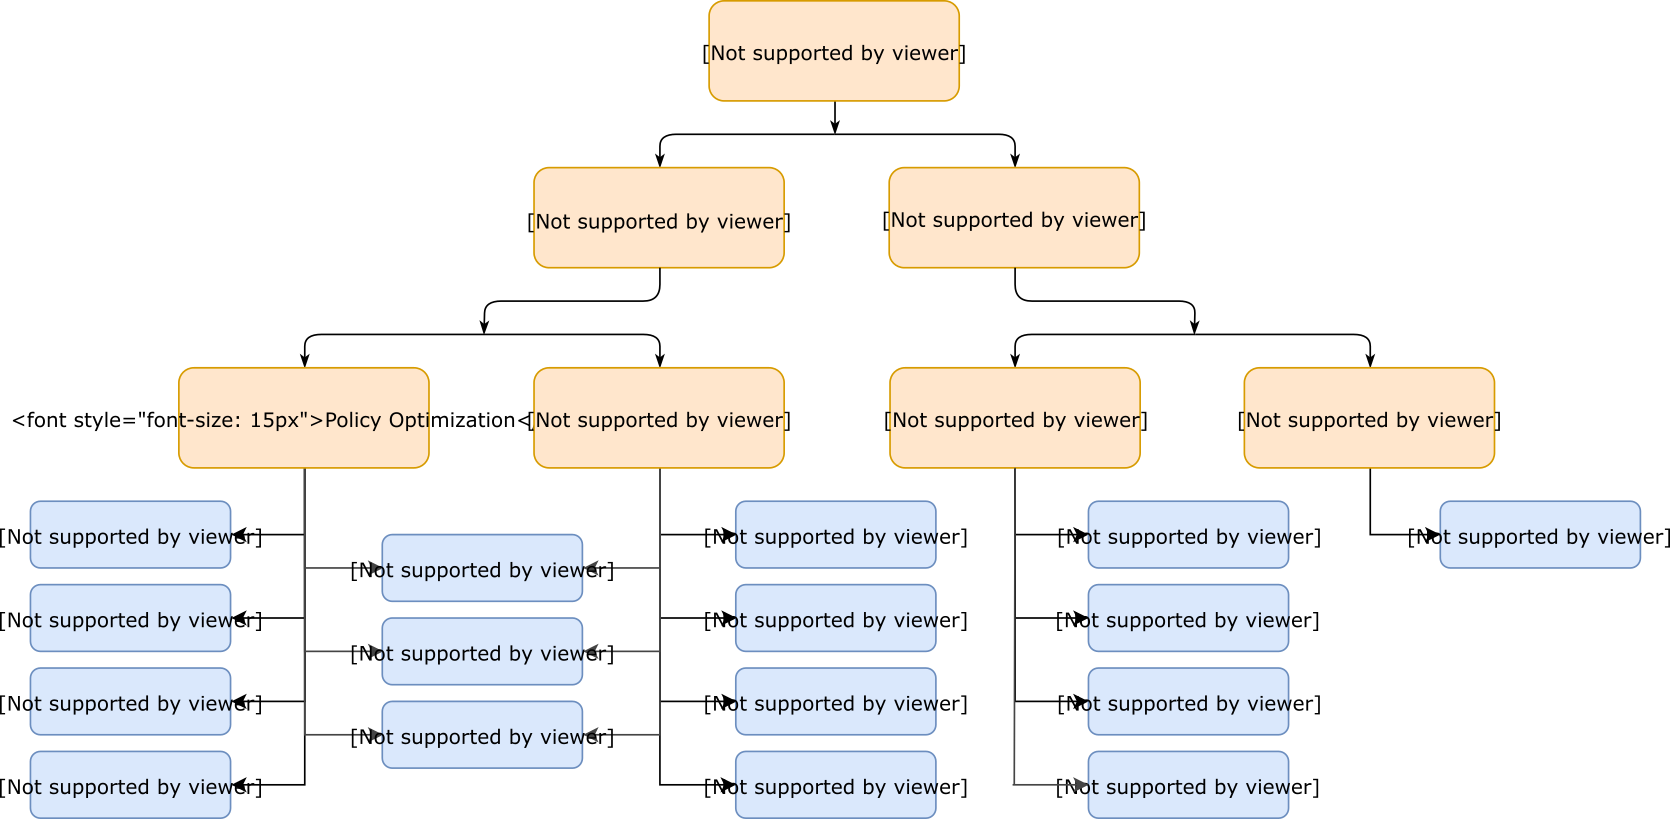
\includegraphics[width=1\textwidth,height=\textheight]{imagenes/reinforcement_learning/rl_algorithms.png}

}

\caption{Esquema Aprendizaje por Refuerzo - Fuente: Propia}

\end{figure}

La primera gran separación se hace sobre si los algoritmos siguen un
modelo definido (model-baed) o no (modelo-free).

\textbf{Model-free}

Por otro lado los \textbf{model-free} usan la experiencia para aprender
o una o ambas de dos cantidades más simples (valores estado/acción o
políticas).

Las aproximaciones de estos algorimtos son de tres tipos:

\begin{itemize}
\tightlist
\item
  \textbf{Policy Optimization}
\end{itemize}

El agente aprende directamente la función política que mapea el estado a
una acción. Nos podemos encontrar con dos tipos de políticas, las
\textbf{políticas deterministicas} (no hay incertidumbre en el mapeo) y
las \textbf{políticas estocásticas} (tenemos una distribución de
probabilidad en las acciones)\textbf{.} En este último caso diremos que
tenemos un Proceso de Decisión de Markov Parcialmente Observable (POMDP,
por sus siglas en ingles).

\begin{itemize}
\tightlist
\item
  \textbf{Q-Learning}
\end{itemize}

En este caso el agente aprende una función valor de acción \(Q(s,a)\)
que nos dirá cómo de bueno es tomar una acción dependiendo del estado.

\begin{itemize}
\tightlist
\item
  \textbf{Híbridos}
\end{itemize}

Estos métodos combinan la fortaleza de los dos métodos anteriores,
aprendiendo tanto la función política como la función valor de acción.

\textbf{Model-based}

Los algoritmos \textbf{model-based} usan la experiencia para construir
un modelo interno de transiciones y resultados inmediatos en el entorno.
Las acciones son elegidas mediante búsqueda o planificación en este
modelo construido.

Las aproximaciones de estos algorimtos son de dos tipos:

\begin{itemize}
\tightlist
\item
  Aprender el Modelo
\end{itemize}

Para aprender el modelo se ejecuta una política base,

\begin{itemize}
\tightlist
\item
  Aprender dado el Modelo
\end{itemize}

Nos centraremos en los algoritmos de tipo \textbf{Model-Free} que son
los más utilizados ya que no requieren del modelo. Si se quieren
profundizar en los diferentes algoritmos, se puede consultar las
documentación en:
\url{https://spinningup.openai.com/en/latest/spinningup/rl_intro2.html\#links-to-algorithms-in-taxonomy}.

Vamos a ver 2 de los algoritmos de tipo \textbf{Model-free} que nos van
a permitir el ver el paso de un algoritmo sin \textbf{Deep Learning} y
otro en el que se aplica \textbf{Deep Learning} para obtener el objetivo
final de tener un \textbf{agente} capaz de aprender por sí solo a
realizar las tareas específicas que se tengan que realizar.

\hypertarget{q-learning-value}{%
\subsection{Q-Learning (value)}\label{q-learning-value}}

Q-Learning es un método basado en valor y que usa el \textbf{sistema TD}
(actualización su función valor en cada paso) para el entrenamiento y su
función de valor de estado.

En nombre de \textbf{Q} viende de \textbf{Quality} (calidad), por que
nos da la calidad de la acción en un determinado estado. Lo que tenemos
es que vamos a tener una \textbf{función de valor de acción (Q-función)}
que nos da un valor numérico de cómo de buena es a partir de un estado
\textbf{s} y una acción \textbf{a}.

En este caso tenemos que internamente nuestra \textbf{Q-función
(}\(Q(s,a)\)\textbf{)} es una \textbf{Q-tabla}, de forma que cada fila
corresponde a un estado, y cada columna a una de las posibles acciones.

\begin{figure}

{\centering 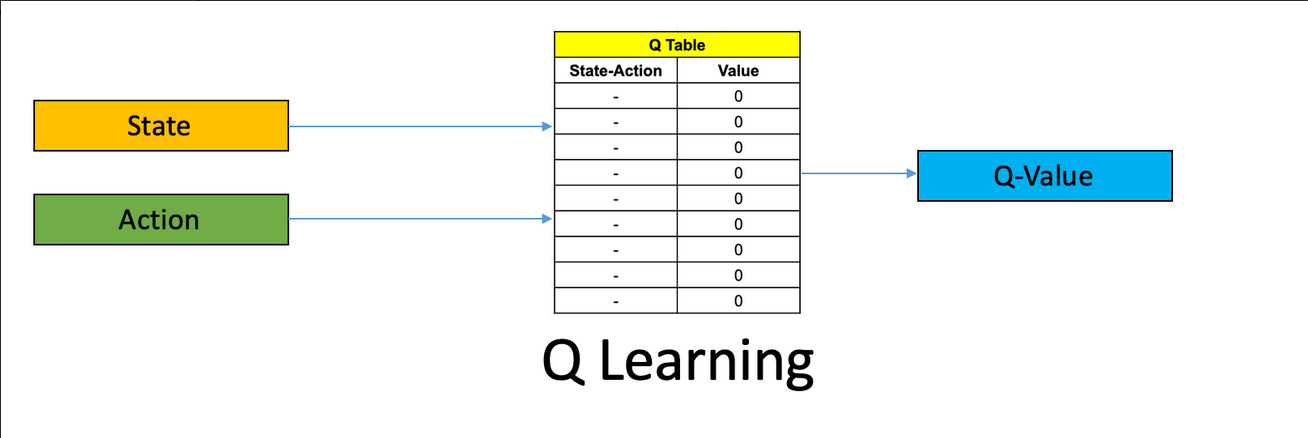
\includegraphics[width=0.5\textwidth,height=\textheight]{imagenes/reinforcement_learning/rl_qlearning.png}

}

\caption{Q-Learning - Fuente:
https://www.analyticsvidhya.com/blog/2019/04/introduction-deep-q-learning-python/}

\end{figure}

Es decir, esta tabla va a contener la información de \textbf{recompensa
total esperada} para cada valor de estado y acción. Cuando nosotros
realizamos el \textbf{entrenamiento} de la Q-función, nosotros
conseguimos una función que \textbf{optimice} esta \textbf{Q-tabla}.

Si nosotros tenemos una Q-función óptima (\(Q^*(s,a)\)), entonces
podremos obtener la \textbf{política óptima} a partir de ella:

\[
\pi^*(s) = \mathop{\mathrm{argmax}}\limits_{a \in \mathcal A}Q^*(s,a)
\] Veamos cuales serían los pasos que deberíamos dar:

\textbf{Inicializamos} nuestra \textbf{Q-Tabla} con valores a 0.
Conforme avanece nuestro entrenamiento estos valores irán cambiando en
función de los datos que se obtengan al \textbf{porbar} a realizar
\textbf{acciones} y obtener las \textbf{recompensas} correspondientes.

El siguiente elemento que necesitamos es una \textbf{política de
entrenamiento} (función que nos permita elegir que acción tomar en
función del estado en el que estemos), en este caso nuestra política
estará basada en los valores de la \textbf{Q-tabla}, es lo que
llamaremos \textbf{explotación} (explotamos la información que tenemos
cogiendo la acción con mejor valor Q) o elegiremos otra acción, es lo
que llamaremos \textbf{exploración} (exploramos nuevos caminos cogiendo
una acción de forma aleatoria).

Esto es lo que se llama una política \(\epsilon\)-greedy, ya que se usa
un parámetro \(\epsilon\), valor entre 0 y 1, que nos permite decidir si
elegimos \textbf{explorar} o si queremos \textbf{explotar} los datos que
ya tenemos.

XXXXX Imagen del gráfico epsilon (epsilon respecto al número de
epsisodios)

Tendremos que:

\begin{itemize}
\tightlist
\item
  con probabilidad 1-\(\epsilon\) nosotros haremos \textbf{explotación}
  y
\item
  con probabilidad \(\epsilon\) nosotros haremos \textbf{exploración}.
\end{itemize}

Es decir, inicialmente le damos valor 1 a \(\epsilon\) de forma que
empezaremos haciendo \textbf{exploración} e iremos bajando este valor de
epsilon conforme avance el entrenamiento para que cada vez usemos más la
\textbf{explotación}.

La idea base es que al principio del entrenamiento, lo prioritario es
\textbf{explorar}, es decir, seleccionar una acción al azar y obtener su
recompensa, ya que nuestra \textbf{Q-Tabla} está inicializada a 0.
Conforme avance el entrenamiento nos tendremos que ir fiando más de los
datos que ya tenemos y tendrá que primar la \textbf{explotación} de
nuestros datos de la \textbf{Q-Tabla}. Para hacer ésto de una forma
efectiva, usaremos un parámetro \textbf{decay\_epsion} que conforme
avancemos en entrenamiento se encargará de ir reduciendo el valor de
\(\epsilon\) para conseguir este efecto.

Una vez que tenemos nuestros elementos base, pasaremos al
\textbf{entrenamiento}, de forma que para todos los \textbf{episodios}
(iteraciones de partidas) que definamos haremos lo siguiente:

\begin{itemize}
\tightlist
\item
  Partimos de un \textbf{estado inicial}, y obtenemos una
  \textbf{acción} a partir de nuestra \textbf{política de entrenamiento}
\item
  Actualizmos \(\epsilon\) con el nuevo valor en este episodio
\item
  Iteramos para un número máximo de pasos dentro de este episodio
\item
  Obtenemos el nuevo estado, así como la recompensa obtenida
\item
  Actulizamos el valor de la \textbf{Q-Tabla} correspondiente según la
  fórmula basada en los métodos de \textbf{TD} (Diferencias temporales)
  \[
  Q(s,a) = Q(s,a) + \alpha(R(s,a)+\gamma argmax_aQ(s',a) - Q(s,a))\\
  \text{donde }s\text{ es el estado actual y }s'\text{ es el nuevo estado}
  \]
\item
  Verificamos si se ha llegado al final del juego para salir de este
  espisodio si es el caso
\item
  Cambiamos el \textbf{estado} como el \textbf{nuevo estado}
\end{itemize}

Una vez acabemos nuestro entrenamiento, obtendremos nuestra
\textbf{política óptima} como: \[
\pi^*(s) = \mathop{\mathrm{argmax}}\limits_{a \in \mathcal A}Q^*(s,a)
\]

\textbf{Pseudo código Q-Learning}

\begin{figure}

{\centering 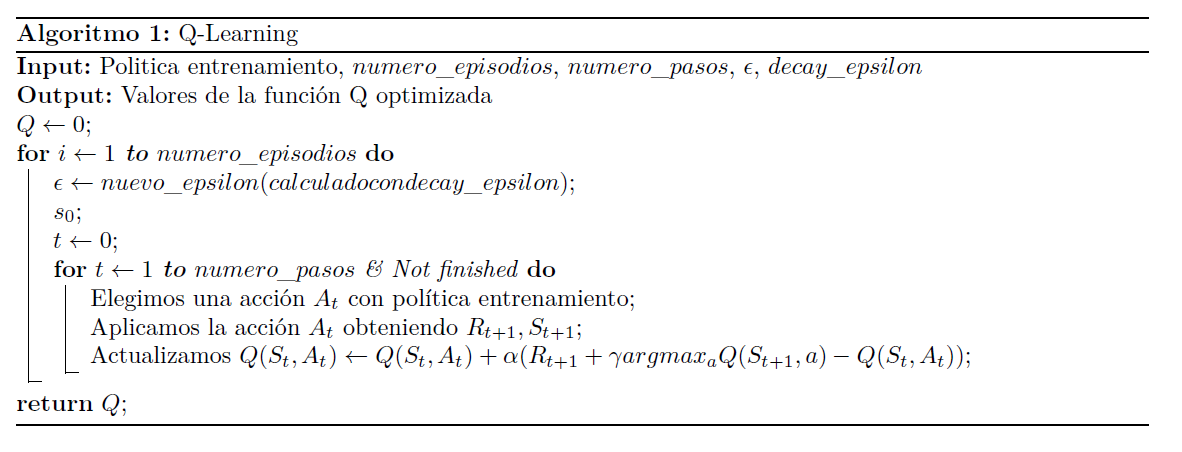
\includegraphics[width=1\textwidth,height=\textheight]{imagenes/reinforcement_learning/rl_algoritmo_qlearning.png}

}

\caption{Algoritmo Q-Learning - Fuente: Propia}

\end{figure}

\hypertarget{dqn-deep-q-learning}{%
\subsection{DQN (Deep Q-Learning)}\label{dqn-deep-q-learning}}

\url{https://www.analyticsvidhya.com/blog/2019/04/introduction-deep-q-learning-python/}

Hemos visto el algoritmo de \textbf{Q-Learning} en el que usábamos una
\textbf{Q-Tabla}, es decir una tabla donde guardábamos todos los valores
de la función \(Q(s,a)\) y que entrenando el agente, éramos capaces de
conseguir aproximar a la función \textbf{Q óptima}, con lo cual teníamos
una \textbf{Política Óptima}.

Este tipo de algoritmos son válidos cuando nos encontramos con un número
``limitado'' de estados y acciones, de forma que la tabla es
relativamente manejable y somos capaces de entrenarla. Si nos
encontramos ante un problema en el que tenemos miles o cientos de miles
de estados no va a ser efectivo construir una tabla y entrenarla para
todas las posibles combinaciones \textbf{etado-acción}. Para abordar
este tipo de problemas, la mejor solución es buscar un
\textbf{aproximador} de la función \(Q(s,a)\), que nos permita obtener
la mejor solución sin necesidad de entrenar todas las posibles
combinaciones.

Para realizar este trabajo una de las posibles opciones es usar
\textbf{redes neuronales} como función aproximadora y que nos abrirá la
posibilidad de trabajar con problemas en los que existan grandes
cantidades de estados/acciones.

Fue el equipo de \textbf{Deepmind} en 2013
(\url{https://www.cs.toronto.edu/~vmnih/docs/dqn.pdf}), en su artítulo
\textbf{``Human-level control through deep reinforcementlearning''}, los
primeros que decidieron atacar los problemas de alta dimensionalidad de
\textbf{estados/acciones} mediante el uso de \textbf{Redes Neuronales
Profundas}. La forma de probar su código fue mediante la implementación
de \textbf{agentes} que fueran capaces de aprender a jugar a los
clásicos \textbf{juegos de Atari 2600}. De forma que el agente,
recibiendo la información de entrada de los pixels que hay en cada
momento en pantalla y el marcador del juego, eran capaces de sobrepasar
el rendimiento de algoritmos actuales que hacían ese trabajo. En estte
caso usaron la misma red neuronal, con la misma arquitectura e
hiperparámetros para los 49 juegos con los que se probaron.

\begin{figure}

{\centering 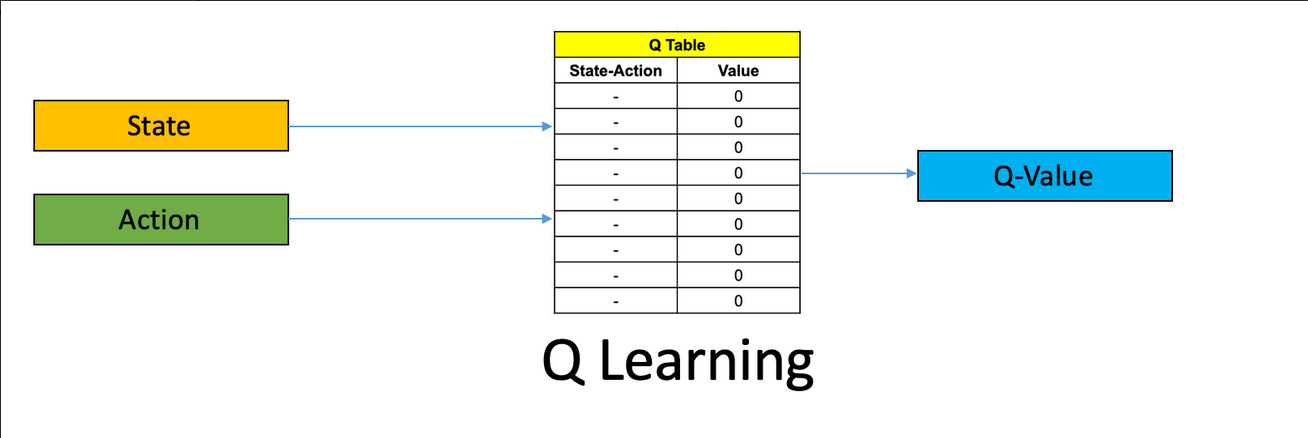
\includegraphics[width=0.5\textwidth,height=\textheight]{imagenes/reinforcement_learning/rl_qlearning.png}

}

\caption{Deep Q-Learning - Fuente:
https://www.analyticsvidhya.com/blog/2019/04/introduction-deep-q-learning-python/}

\end{figure}

Con nuestro algoritmo de \textbf{Q-Learning} teníamos una función
\(Q(s,a)\) que implementábamos con un tabla y nos daba para cada
\textbf{estado} y cada \textbf{acción} cual era el valor de \textbf{Q}
(Quality) de la recompensa esperada. Ahora, con \textbf{Deep Q-Learning}
nos encontramos que vamos a tener una red neuronal que será la encargada
de para cada \textbf{estado} obtener el valor de \textbf{Q} para cada
posible \textbf{acción}.

\textbf{DQN (Deep Q-Network) Arquitectura}

Para poder implementar nuestro trabajo con redes neuronales nos vamos a
encontrar con el problema de entrenar la red neuronal (obtener los
pesos) que permitan alcancar nuestra función \textbf{Q-Óptima} que nos
daría la \textbf{Política Òptima} que es lo que realmente buscamos.

Básicamente para realizar el trabajo usaremos 2 redes neuronales que
tendrán la misma arquitectura de forma que el entrenamiento sea estable.

\begin{itemize}
\tightlist
\item
  \textbf{DQN} que será la red de predicción, y que será la que
  entrenaremos para minimizar el valor del error
  \((R+\gamma argmax_{a'}Q(s',a',w')-Q(s,a,w))^2\)
\item
  \textbf{DQN\_Target} que será la red que calculará
  \(R+\gamma argmax_a'Q(s',a',w')\)
\end{itemize}

\begin{figure}

{\centering 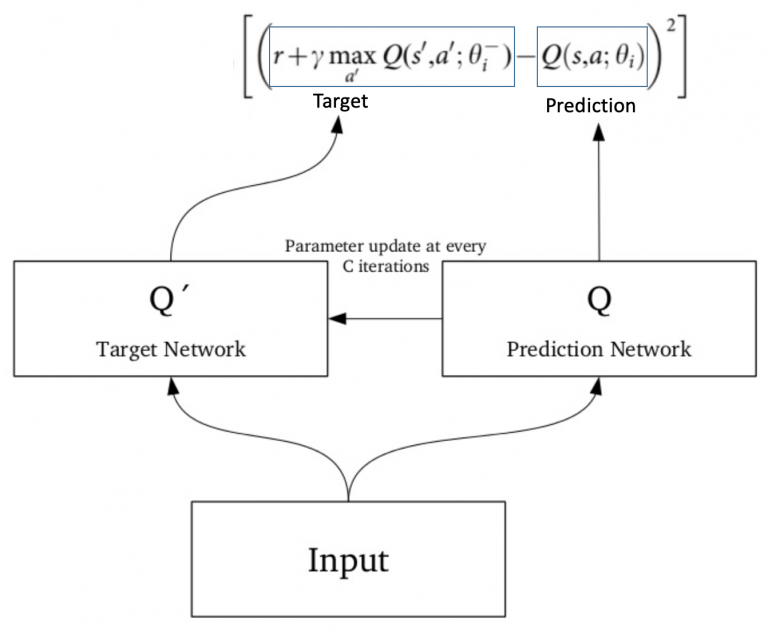
\includegraphics[width=0.5\textwidth,height=\textheight]{imagenes/reinforcement_learning/rl_arquitectura_redes.png}

}

\caption{Arquitectura Redes DQN - Fuente:
https://www.analyticsvidhya.com/blog/2019/04/introduction-deep-q-learning-python/}

\end{figure}

\textbf{Experience Replay}

El mecanismo del \textbf{Experience Replay} nos va a permitir entrenar
nuestra red \textbf{DQN} con minibatchs que vamos a extraer de forma
aleatoria de la memoria en la que vamos a ir guardando los resultados
que vamos obteniendo \textbf{\textless s,a,r,s'\textgreater{}}.

Ésto nos va a permitir por un lado \textbf{entrenar} nuestra \textbf{red
de predicción} y además va a servirnos para evitar
\textbf{correlaciones} de secuencias consecutivas que pudieran producir
un sesgo en nuestros resultados. De esta manera, al elegir al azar los
elementos que vamos a usar para entrenar la red, no tendrán ninguna
relación con los datos consecutivos que se van produciendo en los pasos
de los episodios.

\textbf{Algoritmo Deep Q-Learning}

\begin{itemize}
\tightlist
\item
  Obtenemos los datos de entrada, que es el estado.
\item
  Seleccionamos la acción usando nuestra política de entrenamiento
  epsilon-greedy
\item
  Ejecutamos la acción y obtenemos el siguiente estado así como la
  recompensa obtenida
\item
  Almacenamos en memoria \textless s,a,r,s'\textgreater{}
\item
  Si tenemos bastantes elementos en la memoria

  \begin{itemize}
  \tightlist
  \item
    Hacemos un minibatch aleatorio y enteramos la red siendo
    \(R+\gamma argmax_{a'}Q(s',a',w')\) el \textbf{target de la red} y
    \(Q(s,a,w)\) el valor predicho.
  \item
    La función de pérdida será la de Diferencia de Cuadrados
    \(L = (R+\gamma argmax_a'Q(s',a',w')-Q(s,a,w))^2\)
  \end{itemize}
\item
  Después de cada C iteraciones, copiaremos los pesos de la red DQN a la
  DQN\_Target
\item
  Repetiremos estos pasos durante M episodios
\end{itemize}

\textbf{Pseudo-código Deep Q-Learning}

\begin{figure}

{\centering 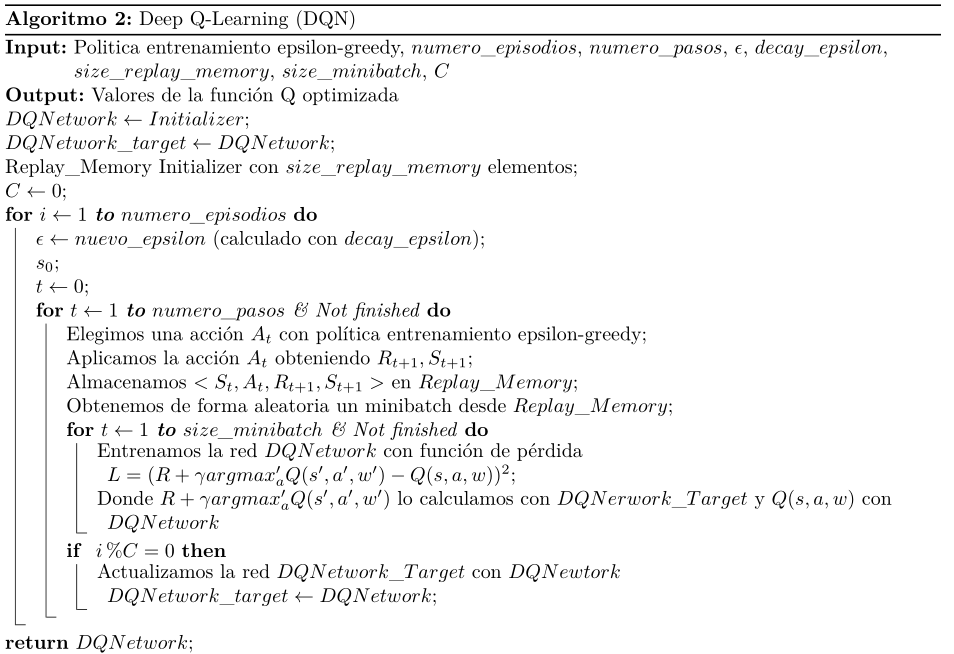
\includegraphics[width=1\textwidth,height=\textheight]{imagenes/reinforcement_learning/rl_algoritmo_dqn.png}

}

\caption{Algoritmo Deep Q-Learning - Fuente: Propia}

\end{figure}

\textbf{Variantes de Deep Q-Learning}

\begin{itemize}
\tightlist
\item
  Double Deep Q Network (DDQN) -- 2015
\item
  Deep Recurrent Q Network (DRQN) -- 2015
\item
  Dueling Q Network -- 2015
\item
  Persistent Advantage Learning (PAL) -- 2015
\item
  Bootstrapped Deep Q Network -- 2016
\item
  Normalized Advantage Functions (NAF) = Continuous DQN -- 2016
\item
  N-Step Q Learning -- 2016
\item
  Noisy Deep Q Network (NoisyNet DQN) -- 2017
\item
  Deep Q Learning for Demonstration (DqfD) -- 2017
\item
  Categorical Deep Q Network = Distributed Deep Q Network = C51 -- 2017

  \begin{itemize}
  \tightlist
  \item
    Rainbow -- 2017
  \end{itemize}
\item
  Quantile Regression Deep Q Network (QR-DQN) -- 2017
\item
  Implicit Quantile Network -- 2018
\end{itemize}

\hypertarget{listado-algoritmos}{%
\subsection{Listado Algoritmos}\label{listado-algoritmos}}

\textbf{1. Model-Free}

\textbf{Value-based}

\href{https://link.springer.com/content/pdf/10.1007/BF00992698.pdf}{Q-learning
= SARSA max} -- 1992

\href{http://mi.eng.cam.ac.uk/reports/svr-ftp/auto-pdf/rummery_tr166.pdf}{State
Action Reward State-Action (SARSA)}-- 1994

\href{https://www.cs.toronto.edu/~vmnih/docs/dqn.pdf}{Deep Q Network
(DQN)} -- 2013

\href{https://arxiv.org/pdf/1509.06461.pdf}{Double Deep Q Network
(DDQN)} -- 2015

\href{https://arxiv.org/abs/1507.06527}{Deep Recurrent Q Network (DRQN)}
-- 2015

\href{https://arxiv.org/abs/1511.06581}{Dueling Q Network} -- 2015

\href{https://arxiv.org/abs/1512.04860}{Persistent Advantage Learning
(PAL)} -- 2015

\href{https://arxiv.org/abs/1602.04621}{Bootstrapped Deep Q Network} --
2016

\href{https://arxiv.org/abs/1603.00748}{Normalized Advantage Functions
(NAF) = Continuous DQN} -- 2016

\href{https://arxiv.org/abs/1602.01783}{N-Step Q Learning} -- 2016

\href{https://arxiv.org/abs/1706.10295}{Noisy Deep Q Network (NoisyNet
DQN)} -- 2017

\href{https://arxiv.org/abs/1704.03732}{Deep Q Learning for
Demonstration (DqfD)} -- 2017

\href{https://arxiv.org/abs/1707.06887}{Categorical Deep Q Network =
Distributed Deep Q Network = C51} -- 2017

\begin{itemize}
\tightlist
\item
  \href{https://arxiv.org/abs/1710.02298}{Rainbow} -- 2017
\end{itemize}

\href{https://arxiv.org/pdf/1710.10044v1.pdf}{Quantile Regression Deep Q
Network (QR-DQN)} -- 2017

\href{https://arxiv.org/abs/1806.06923}{Implicit Quantile Network}--
2018

\href{https://arxiv.org/abs/1703.01310}{Mixed Monte Carlo (MMC)} -- 2017

\href{https://arxiv.org/abs/1703.01988}{Neural Episodic Control (NEC)}
-- 2017

\textbf{Policy-based}

\href{https://link.springer.com/article/10.1023/A:1010091220143}{Cross-Entropy
Method (CEM)}-- 1999

Policy Gradient

\begin{itemize}
\tightlist
\item
  \href{https://people.cs.umass.edu/~barto/courses/cs687/williams92simple.pdf}{REINFORCE
  = Vanilla Policy Gradient}(VPG)- 1992
\item
  Policy gradient softmax
\item
  \href{https://papers.nips.cc/paper/2073-a-natural-policy-gradient.pdf}{Natural
  Policy Gradient (Optimisation) (NPG) / (NPO)} -- 2002
\item
  \href{https://arxiv.org/abs/1604.06778}{Truncated Natural Policy
  Gradient (TNPG)} -- 2016
\end{itemize}

\textbf{Actor-Critic}

\href{https://arxiv.org/abs/1602.01783}{Advantage Actor Critic (A2C)} --
2016

\href{https://arxiv.org/abs/1602.01783}{Asynchronous Advantage
Actor-Critic (A3C)}~ -- 2016

\href{https://arxiv.org/abs/1506.02438}{Generalized Advantage Estimation
(GAE)} -- 2015

\href{https://arxiv.org/abs/1502.05477}{Trust Region Policy Optimization
(TRPO)} -- 2015

\href{http://proceedings.mlr.press/v32/silver14.pdf}{Deterministic
Policy Gradient (DPG)} -- 2014

\href{https://arxiv.org/abs/1509.02971}{Deep Deterministic Policy
Gradients (DDPG)}~ -- 2015

\begin{itemize}
\tightlist
\item
  \href{https://arxiv.org/abs/1804.08617}{Distributed Distributional
  Deterministic Policy Gradients (D4PG)} -- 2018
\item
  \href{https://arxiv.org/pdf/1802.09477.pdf}{Twin Delayed Deep
  Deterministic Policy Gradient (TD3)} -- 2018
\end{itemize}

\href{https://arxiv.org/abs/1611.01224}{Actor-Critic with Experience
Replay (ACER)} -- 2016

\href{https://arxiv.org/abs/1708.05144}{Actor Critic using
Kronecker-Factored Trust Region (ACKTR)} -- 2017

\href{https://arxiv.org/abs/1707.06347}{Proximal Policy Optimization
(PPO)~}-- 2017

\begin{itemize}
\tightlist
\item
  \href{https://arxiv.org/abs/1707.02286}{Distributed PPO (DPPO)} --
  2017
\item
  \href{https://arxiv.org/pdf/1707.06347.pdf}{Clipped PPO (CPPO)}~ --
  2017
\item
  \href{https://arxiv.org/abs/1911.00357}{Decentralized Distributed PPO
  (DD-PPO)}-- 2019
\end{itemize}

\href{https://arxiv.org/abs/1801.01290}{Soft Actor-Critic (SAC)}~ --
2018

\textbf{General Agents}

\begin{itemize}
\tightlist
\item
  \href{https://ieeexplore.ieee.org/document/542381}{Covariance Matrix
  Adaptation Evolution Strategy (CMA-ES)}-- 1996
\item
  \href{https://papers.nips.cc/paper/3545-policy-search-for-motor-primitives-in-robotics.pdf}{Episodic
  Reward-Weighted Regression (ERWR)} -- 2009
\item
  \href{https://www.aaai.org/ocs/index.php/AAAI/AAAI10/paper/viewFile/1851/2264}{Relative
  Entropy Policy Search (REPS)}-- 2010
\item
  \href{https://arxiv.org/abs/1611.01779}{Direct Future Prediction
  (DFP)} -- 2016
\end{itemize}

\textbf{Imitation Learning Agents}

Behavioral Cloning (BC)

\href{https://www.cs.cmu.edu/~sross1/publications/Ross-AIStats11-NoRegret.pdf}{Dataset
Aggregation (Dagger)} (i.e.~query the expert) -- 2011

Adversarial Reinforcement Learning

\begin{itemize}
\tightlist
\item
  \href{https://arxiv.org/abs/1606.03476}{Generative Adversarial
  Imitation Learning (GAIL)} -- 2016
\item
  \href{https://arxiv.org/abs/1710.11248}{Adverserial Inverse
  Reinforcement Learning (AIRL)}-- 2017
\end{itemize}

\href{https://arxiv.org/abs/1710.02410}{Conditional Imitation Learning}
-- 2017

\href{https://arxiv.org/abs/1905.11108}{Soft Q-Imitation Learning
(SQIL)} -- 2019

\textbf{Hierarchical Reinforcement Learning Agents}

\begin{itemize}
\tightlist
\item
  \href{https://arxiv.org/abs/1712.00948.pdf}{Hierarchical Actor Critic
  (HAC)} -- 2017
\end{itemize}

\textbf{Memory Types}

\begin{itemize}
\tightlist
\item
  \href{https://arxiv.org/abs/1511.05952}{Prioritized Experience Replay
  (PER)} -- 2015
\item
  \href{https://arxiv.org/abs/1707.01495.pdf}{Hindsight Experience
  Replay (HER)} -- 2017
\end{itemize}

\textbf{Exploration Techniques}

\begin{itemize}
\tightlist
\item
  E-Greedy
\item
  Boltzmann
\item
  Ornstein--Uhlenbeck process
\item
  Normal Noise
\item
  Truncated Normal Noise
\item
  \href{https://arxiv.org/abs/1602.04621}{Bootstrapped Deep Q Network}~
\item
  \href{https://arxiv.org/abs/1706.01502}{UCB Exploration via
  Q-Ensembles (UCB)}~
\item
  \href{https://arxiv.org/abs/1706.10295}{Noisy Networks for
  Exploration}~
\item
  \href{https://pathak22.github.io/noreward-rl/}{Intrinsic Curiosity
  Module (ICM)} -- 2017
\end{itemize}

\textbf{Meta Learning}

\begin{itemize}
\tightlist
\item
  \href{https://arxiv.org/abs/1703.03400}{Model-agnostic meta-learning
  (MAML)}-- 2017
\item
  \href{https://openreview.net/pdf?id=S1evHerYPr}{Improving
  Generalization in Meta Reinforcement Learning using Learned
  Objectives} (MetaGenRLis) -- 2020
\end{itemize}

\textbf{2. Model-Based}

\textbf{Dyna-Style Algorithms / Model-based data generation}

\begin{itemize}
\tightlist
\item
  \href{http://citeseerx.ist.psu.edu/viewdoc/download?doi=10.1.1.51.7362\&rep=rep1\&type=pdf}{Dynamic
  Programming (DP) = DYNA-Q} -- 1990
\item
  \href{https://arxiv.org/abs/1506.07365}{Embed to Control (E2C)}-- 2015
\item
  \href{https://arxiv.org/abs/1802.10592}{Model-Ensemble Trust-Region
  Policy Optimization (ME-TRPO)} -- 2018
\item
  \href{https://arxiv.org/abs/1807.03858}{Stochastic Lower Bound
  Optimization (SLBO)} -- 2018
\item
  \href{https://arxiv.org/abs/1809.05214}{Model-Based
  Meta-Policy-Optimzation (MB-MPO)} (meta learning) -- 2018
\item
  \href{https://arxiv.org/abs/1803.00101}{Stochastic Ensemble Value
  Expansion (STEVE)} -- 2018
\item
  \href{https://arxiv.org/abs/1803.00101}{Model-based Value Expansion
  (MVE)} -- 2018
\item
  \href{https://arxiv.org/abs/1903.00374}{Simulated Policy Learning
  (SimPLe)} -- 2019
\item
  \href{https://arxiv.org/abs/1906.08253}{Model Based Policy
  Optimization (MBPO)} -- 2019
\end{itemize}

\textbf{Policy Search with Backpropagation through Time / Analytic
gradient computation}

\begin{itemize}
\tightlist
\item
  \href{https://www.jstor.org/stable/3613752?origin=crossref\&seq=1}{Differential
  Dynamic Programming (DDP)} -- 1970
\item
  \href{http://users.cecs.anu.edu.au/~john/papers/BOOK/B03.PDF}{Linear
  Dynamical Systems and Quadratic Cost (LQR)} -- 1989
\item
  \href{https://homes.cs.washington.edu/~todorov/papers/LiICINCO04.pdf}{Iterative
  Linear Quadratic Regulator (ILQR)} -- 2004
\item
  \href{https://www.ias.informatik.tu-darmstadt.de/uploads/Publications/Deisenroth_ICML_2011.pdf}{Probabilistic
  Inference for Learning Control (PILCO)} -- 2011
\item
  \href{https://homes.cs.washington.edu/~todorov/papers/TassaIROS12.pdf}{Iterative
  Linear Quadratic-Gaussian (iLQG)} -- 2012
\item
  \href{http://citeseerx.ist.psu.edu/viewdoc/download?doi=10.1.1.716.4271\&rep=rep1\&type=pdf}{Approximate
  iterative LQR with Gaussian Processes (AGP-iLQR)} -- 2014
\item
  \href{https://graphics.stanford.edu/projects/gpspaper/gps_full.pdf}{Guided
  Policy Search (GPS)} -- 2013
\item
  \href{https://arxiv.org/abs/1510.09142}{Stochastic Value Gradients
  (SVG)} -- 2015
\item
  \href{https://dl.acm.org/doi/10.5555/3306127.3331874}{Policy search
  with Gaussian Process} -- 2019
\end{itemize}

\textbf{Shooting Algorithms / sampling-based planning}

\href{https://arxiv.org/pdf/1708.02596.pdf}{Random Shooting (RS)} --
2017

\href{https://www.sciencedirect.com/science/article/pii/B9780444538598000035}{Cross-Entropy
Method (CEM)}-- 2013

\begin{itemize}
\tightlist
\item
  \href{https://arxiv.org/abs/1811.04551}{Deep Planning Network
  (DPN)}-2018
\item
  \href{https://arxiv.org/abs/1805.12114}{Probabilistic Ensembles with
  Trajectory Sampling (PETS-RS and PETS-CEM)} -- 2018
\item
  \href{https://arxiv.org/abs/1610.00696}{Visual Foresight} -- 2016
\end{itemize}

\href{https://arxiv.org/abs/1509.01149}{Model Predictive Path Integral
(MPPI)} -- 2015

\begin{itemize}
\tightlist
\item
  \href{https://arxiv.org/abs/1909.11652}{Planning with Deep Dynamics
  Models (PDDM)} -- 2019
\end{itemize}

\href{https://hal.inria.fr/inria-00116992/document}{Monte-Carlo Tree
Search (MCTS)} -- 2006

\begin{itemize}
\tightlist
\item
  \href{https://arxiv.org/abs/1712.01815}{AlphaZero} -- 2017
\end{itemize}

~

\hypertarget{redes-generativas-adversarias}{%
\section{Redes Generativas
Adversarias}\label{redes-generativas-adversarias}}

\hypertarget{actualidad-y-algunos-conceptos-relacionados-con-el-deep-learning}{%
\section{Actualidad y algunos conceptos relacionados con el Deep
Learning}\label{actualidad-y-algunos-conceptos-relacionados-con-el-deep-learning}}

\hypertarget{software-para-aplicar-deep-learning}{%
\section{Software para aplicar Deep
Learning}\label{software-para-aplicar-deep-learning}}

\bookmarksetup{startatroot}

\hypertarget{anuxe1lisis-causal-y-modelos-gruxe1ficos-probabiluxedsticos}{%
\chapter{Análisis Causal y Modelos Gráficos
Probabilísticos}\label{anuxe1lisis-causal-y-modelos-gruxe1ficos-probabiluxedsticos}}

\hypertarget{relaciones-y-modelos-causales}{%
\section{Relaciones y Modelos
Causales}\label{relaciones-y-modelos-causales}}

\hypertarget{redes-bayesianas-aprendizaje-y-clasificadores}{%
\section{Redes bayesianas: aprendizaje y
clasificadores}\label{redes-bayesianas-aprendizaje-y-clasificadores}}

\hypertarget{hipuxf3tesis-map-y-naive-bayes}{%
\subsection{Hipótesis MAP y
Naive-Bayes}\label{hipuxf3tesis-map-y-naive-bayes}}

\hypertarget{modelos-bayesianos}{%
\subsection{Modelos bayesianos}\label{modelos-bayesianos}}

\hypertarget{modelos-ocultos-de-markov}{%
\section{Modelos Ocultos de Markov}\label{modelos-ocultos-de-markov}}

\hypertarget{tipos-de-cadenas-de-markov}{%
\subsection{Tipos de cadenas de
Markov}\label{tipos-de-cadenas-de-markov}}

\hypertarget{aplicaciones-de-moms}{%
\subsection{Aplicaciones de MOMs}\label{aplicaciones-de-moms}}

\hypertarget{causal-machine-learning}{%
\section{Causal Machine Learning}\label{causal-machine-learning}}

\hypertarget{efectos-causales.-ate-y-cate}{%
\subsection{Efectos causales. ATE y
CATE}\label{efectos-causales.-ate-y-cate}}

\hypertarget{uplift}{%
\subsection{Uplift}\label{uplift}}

\bookmarksetup{startatroot}

\hypertarget{algoritmos-genuxe9ticos}{%
\chapter{Algoritmos Genéticos}\label{algoritmos-genuxe9ticos}}

Buenas referencias
https://repository.urosario.edu.co/server/api/core/bitstreams/7ae959ec-81de-435b-aca4-e9bb365e4894/content

Buena documentación (graficos)

https://www.cs.us.es/\textasciitilde fsancho/Blog/posts/Algoritmos\_Geneticos.md.html

http://www.robolabo.etsit.upm.es/asignaturas/irin/transparencias/AG.pdf

http://www.sc.ehu.es/ccwbayes/docencia/mmcc/docs/temageneticos.pdf

https://sci2s.ugr.es/sites/default/files/files/Teaching/GraduatesCourses/Bioinformatica/Tema\%2006\%20-\%20AGs\%20I.pdf

Individuo o Cromosoma Compuesto de Genes Codificación de genes (Binaria,
Entera, Real)

\hypertarget{introducciuxf3n-4}{%
\section{Introducción}\label{introducciuxf3n-4}}

Los algoritmos genéticos es un método bastante común en minería de
datos. Se inspiran en el \textbf{proceso natural de selección y
evolución} tal y como se describe por la teoría evolucionista de la
selección natural postulada por \textbf{Darwin}.

Los \textbf{principios} sobre los que se asientan los algoritmos
genéticos son:

\begin{itemize}
\item
  Los individuos \textbf{mejor adaptados} al entorno son aquellos que
  tienen una probabilidad mayor de \textbf{sobrevivir} y, por ende, de
  \textbf{reproducirse}.
\item
  Los descendientes \textbf{heredan} características de sus
  progenitores.
\item
  De forma esporádica y natural se producen \textbf{mutaciones} en el
  material genético de algunos individuos, provocando cambios
  permanentes.
\end{itemize}

Los algoritmos genéticos son adecuados para obtener buenas
aproximaciones en \textbf{problemas de búsqueda, aprendizaje y
optimización} {[}Marczyk. 2004{]}.

De forma esquemática un algoritmo genético es una \textbf{función
matemática} que tomando como entrada unos individuos iniciales
(\textbf{población origen}) selecciona aquellos \textbf{ejemplares}
(también llamados individuos o cromosomas) que \textbf{recombinándose}
por algún método generarán como resultado la \textbf{siguiente
generación}. Esta función se aplicará de forma \textbf{iterativa} hasta
verificar alguna condición de parada, bien pueda ser un número máximo de
iteraciones o bien la obtención de un individuo que cumpla unas
restricciones iniciales.

\textbf{Condiciones para la aplicación de los Algoritmos Genéticos}

No es posible la aplicación en toda clase de problemas de los algoritmos
genéticos. Para que estos puedan aplicarse, los problemas deben cumplir
las siguientes condiciones:

\begin{itemize}
\item
  El \textbf{espacio de búsqueda} \footnote{\textbf{Recordemos que
    cualquier método de Data Mining se puede asimilar como una búsqueda
    en el espacio solución, es decir, el espacio formado por todas las
    posibles soluciones de un problema}} debe estar acotado, por tanto
  ser \textbf{finito}.
\item
  Es necesario poseer una \textbf{función} de aptitud, que denominaremos
  \textbf{fitness}, que evalúe cada solución (individuo) indicándonos de
  forma cuantitativa cuán buena o mala es una solución concreta.
\item
  Las \textbf{soluciones} deben ser \textbf{codificables} en un lenguaje
  comprensible para un \textbf{ordenador}, y si es posible de la forma
  más \textbf{compacta} y abreviada posible.
\end{itemize}

Habitualmente, la segunda condición es la más complicada de conseguir,
para ciertos problemas es trivial la función de fitness (por ejemplo, en
el caso de la búsqueda del máximo de una función) no obstante, en la
vida real a veces es muy complicada de obtener y, habitualmente, se
realizan conjeturas evaluándose los algoritmos con varias funciones de
fitness.

\textbf{Ventajas e inconvenientes}

\textbf{Ventajas}

\begin{itemize}
\item
  No necesitan ningún conocimiento particular del problema sobre el que
  trabajan, únicamente cada ejemplar debe representar una posible
  solución al problema.
\item
  Es un algoritmo admisible, es decir, con un número de iteraciones
  suficiente son capaces de obtener la solución óptima en problemas de
  optimización.
\item
  Los algoritmos genéticos son bastante robustos frente a falsas
  soluciones ya que al realizar una inspección del espacio solución de
  forma no lineal (por ejemplo, si quisiéramos obtener el máximo
  absoluto de una función) el algoritmo no recorre la función de forma
  consecutiva por lo que no se ve afectada por máximos locales.
\item
  Altamente paralelizable, es decir, ya que el cálculo no es lineal
  podemos utilizar varias máquinas para ejecutar el programa y evaluar
  así un mayor número de casos.
\item
  Pueden ser incrustrables en muchos algoritmos de data mining para
  formar modelos híbridos. Por ejemplo para seleccionar el número óptimo
  de neuronas en un modelo de Perceptrón Multicapa.
\end{itemize}

\textbf{Inconvenientes}

\begin{itemize}
\item
  Su coste computacional puede llegar a ser muy elevado, si el espacio
  de trabajo es muy grande.
\item
  En el caso de que no se haga un correcto ajuste de los parámetros
  pueden llegar a caer en una situación de dominación en la que se
  produce un bucle infinito ya que unos individuos dominan sobre los
  demás impidiendo la evolución de la población y por tanto inhiben la
  diversidad biológica.
\item
  Puede llegar a ser muy complicado encontrar una función de evaluación
  de cada uno de los individuos para seleccionar los mejores de los
  peores.
\end{itemize}

\hypertarget{fundamentos-teuxf3ricos-conceptos}{%
\section{Fundamentos teóricos
(conceptos)}\label{fundamentos-teuxf3ricos-conceptos}}

A continuación, se explican, someramente, los conceptos básicos de los
algoritmos genéticos.

\hypertarget{codificaciuxf3n-de-los-datos}{%
\subsection{Codificación de los
datos}\label{codificaciuxf3n-de-los-datos}}

Cada \textbf{individuo o cromosoma} está formado por unos cuantos
\textbf{genes}. Estos individuos con sus genes los tenemos que
representar de forma que podamos codificar esa información.

Los principales métodos de representación son: - \textbf{Binaria:} Los
individuos/cromosomas están representados por una serie de genes que son
bits ( valores 0 ó 1).

\begin{itemize}
\item
  \textbf{Entera:} Los individuos/cromosomas están representados por una
  serie de genes que son números enteros.
\item
  \textbf{Real:} Los individuos/cromosomas están representados por una
  serie de genes que son números reales en coma flotante.
\item
  \textbf{Permutacional:} Los individuos/cromosomas están representados
  por una serie de genes que son permutaciones de un conjunto de
  elementos. Se usan en aquellos problemas en los que la secuencia u
  orden es importante.
\item
  \textbf{Basada en árboles:} Los individuos/cromosomas están
  representados por una serie de genes que son estructuras jerárquicas.
\end{itemize}

El primer paso para conseguir que un ordenador procese unos
\textbf{datos} es conseguir \textbf{representarlos} de una forma
apropiada. En primer término, para codificar los datos, es necesario
separar las posibles configuraciones posibles del dominio del problema
en un \textbf{conjunto} de \textbf{estados} \textbf{finito}.

Una vez obtenida esta clasificación el objetivo es representar cada
\textbf{estado} de \textbf{forma} \textbf{unívoca} con una cadena de
caracteres (compuesta en la mayoría de casos por unos y ceros).

A pesar de que cada estado puede codificarse con alfabetos de diferente
cardinalidad\footnote{La longitud de las cadenas que representen los
  posibles estados no es necesario que sea fija, representaciones como
  la de Kitano para representar operaciones matemáticas son un ejemplo
  de esto}, uno de los resultados fundamentales de la teoría de
algoritmos genéticos es el \textbf{teorema del esquema}, que afirma que
la codificación \textbf{óptima} es aquella en la que los algoritmos
tienen un alfabeto de cardinalidad, es decir el uso del
\textbf{alfabeto} \textbf{binario}.

El enunciado del \textbf{teorema} del \textbf{esquema} es el siguiente:
«\emph{Esquemas cortos, de bajo orden y aptitud superior al promedio
reciben un incremento exponencial de representantes en generaciones
subsecuentes de un Algoritmo Genético.}»

Una de las ventajas de usar un alfabeto binario para la construcción de
configuraciones de estados es la sencillez de los operadores utilizados
para la modificación de estas. En el caso de que el alfabeto sea
binario, los operadores se denominan, lógicamente, \textbf{operadores}
\textbf{binarios}. Es importante destacar que variables que estén
próximas en el espacio del problema deben preferiblemente estarlo en la
codificación ya que la proximidad entre ellas condiciona un elemento
determinante en la mutación y reproducibilidad de éstas. Es decir, dos
estados que en nuestro espacio de estados del universo del problema que
están consecutivos deberían estarlo en la representación de los datos,
esto es útil para que cuando haya mutaciones los saltos se den entre
estados consecutivos. En términos generales cumplir esta premisa mejora
experimentalmente los resultados obtenidos con algoritmos genéticos.

En la práctica el factor que condiciona en mayor grado el fracaso o el
\textbf{éxito} de la aplicación de algoritmos genéticos a un problema
dado es una \textbf{codificación} \textbf{acorde} con los
\textbf{datos}.

Otra opción muy común es establecer a cada uno de los posibles casos un
\textbf{número} \textbf{natural} y luego codificar ese número en binario
natural, de esta forma minimizamos el problema que surge al concatenar
múltiples variables independientes en el que su representación binaria
diera lugar a numerosos huecos que produjeran soluciones no válidas. Por
ejemplo, tenemos 3 variables, las dos primeras tienen 3 posibles estados
y la última dos, el número posible de estados es 3+3+2 = 8, combinando
las 3 variables podemos codificar todo con 3 bits en comparación con los
2+2+1 = 5 bits necesarios que utilizaríamos en el caso de realizar el
procedimiento anterior. En este ejemplo no sólo ahorraríamos espacio
sino que además evitaríamos que se produjeran individuos cuya solución
no es factible.

\hypertarget{algoritmo}{%
\subsection{Algoritmo}\label{algoritmo}}

Un algoritmo genético implementado en \textbf{pseudo código} podría ser
el siguiente:

\texttt{Generar\ de\ forma\ aleatoria\ una\ población\ inicial\ aleatoria.\ Cada\ individuo/cromosoma\ tiene\ sus\ propios\ genes.}

\texttt{Mientras\ (condición\ de\ terminación\ es\ falsa).}

\texttt{Evaluar\ el\ fitness\ de\ cada\ uno\ de\ los\ individuos.}

\texttt{Selección\ de\ los\ individuos\ con\ mejor\ fitness.}

\texttt{Recombinación\ de\ los\ individuos.}

\texttt{Mutación\ de\ los\ indiviudos.}

Un posible esquema que puede representar una posible implementación de
algoritmos genéticos se muestra en la figura
Figure~\ref{fig-esquema-genetico} .

\begin{figure}

{\centering 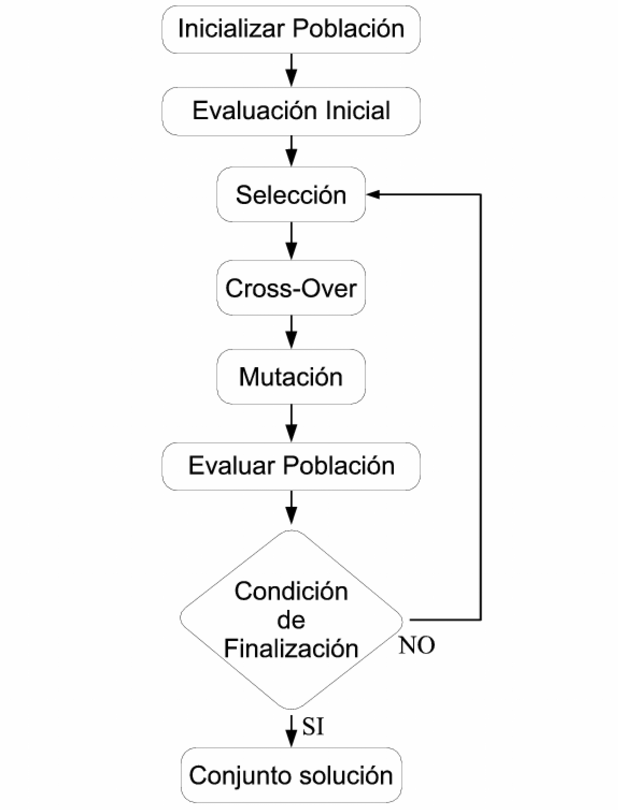
\includegraphics{imagenes/capitulo3/esquema_genetico.png}

}

\caption{\label{fig-esquema-genetico}Esquema de implementación de un
algoritmo genético}

\end{figure}

A continuación, en los siguientes apartados, se hará una descripción de
las fases anteriormente expuestas:

\textbf{Inicializar Población}

Como ya se ha explicado antes el primer paso es inicializar la población
origen. Habitualmente la inicialización se hace de forma
\textbf{aleatoria} procurando una \textbf{distribución}
\textbf{homogénea} en los casos iniciales de prueba. No obstante, si se
tiene un conocimiento más profundo del problema es posible obtener
mejores resultados inicializando la población de una forma apropiada a
la clase de soluciones que se esperan obtener.

\textbf{Evaluar Población}

Durante cada \textbf{iteración} (generación) cada gen se decodifica
convirtiéndose en un grupo de parámetros del problema y se evalúa el
problema con esos datos.

Pongamos por ejemplo que queremos evaluar el máximo de la función
\(f(x)=x²\) en el intervalo \([0,1]\) y supongamos que construimos cada
gen con \textbf{6 dígitos} \((2^6=64)\) , por lo que interpretando el
número obtenido en binario natural y dividiéndolo entre 64 obtendremos
el punto de la función que corresponde al gen (individuo). Evaluando
dicho punto en la función que queremos evaluar (\(f(x)=x²\)) obtenemos
lo que en nuestro caso sería el \textbf{fitness}, en este caso cuanto
mayor fitness tenga un gen mejor valorado está y más probable es que
prospere su descendencia en el futuro. No en todas las implementaciones
de algoritmos genéticos se realiza una fase de evaluación de la
población tal y como aquí está descrita, en ciertas ocasiones se omite y
no se genera ningún fitness asociado a cada estado evaluado. Selección
La fase de selección elije los individuos a reproducirse en la próxima
generación, esta selección puede realizarse por muy distintos métodos.

En el algoritmo mostrado en pseudo código anteriormente el
\textbf{método} de \textbf{selección} usado depende del fitness de cada
individuo. A continuación, se describen los más comunes:

\textbf{Selección elitista:} Se seleccionan los individuos con mayor
fitness de cada generación. La mayoría de los algoritmos genéticos no
aplican un elitismo puro, sino que en cada generación evalúan el fitness
de cada uno de los individuos, en el caso de que los mejores de la
anterior generación sean mejores que los de la actual éstos se copian
sin recombinación a la siguiente generación.

\textbf{Selección proporcional a la aptitud:} los individuos más aptos
tienen más probabilidad de ser seleccionados, asignándoles una
probabilidad de selección más alta. Una vez seleccionadas las
probabilidades de selección a cada uno de los individuos se genera una
nueva población teniendo en cuenta éstas.

\textbf{Selección por rueda de ruleta:} Es un método conceptualmente
similar al anterior. Se le asigna una probabilidad absoluta de aparición
de cada individuo de acuerdo al fitness de forma que ocupe un tramo del
intervalo total de probabilidad (de 0 a 1) de forma acorde a su fitness.
Una vez completado el tramo total se generan números aleatorios de 0 a 1
de forma que se seleccionen los individuos que serán el caldo de cultivo
de la siguiente generación.

\textbf{Selección por torneo:} se eligen subgrupos de individuos de la
población, y los miembros de cada subgrupo compiten entre ellos. Sólo se
elige a un individuo de cada subgrupo para la reproducción.

\textbf{Selección por rango:} a cada individuo de la población se le
asigna un rango numérico basado en su fitness, y la selección se basa en
este ranking, en lugar de las diferencias absolutas en el fitness. La
ventaja de este método es que puede evitar que individuos muy aptos
ganen dominancia al principio a expensas de los menos aptos, lo que
reduciría la diversidad genética de la población y podría obstaculizar
la búsqueda de una solución aceptable.

Un ejemplo de esto podría ser que al intentar maximizar una función el
algoritmo genético convergiera hacía un máximo local que posee un
fitness mucho mejor que el de sus congéneres de población lo que haría
que hubiera una dominancia clara con la consecuente desaparición de los
individuos menos aptos (con peor fitness).

\textbf{Selección generacional}: la descendencia de los individuos
seleccionados en cada generación se convierte en la siguiente
generación. No se conservan individuos entre las generaciones.

\textbf{Selección por estado estacionario:} la descendencia de los
individuos seleccionados en cada generación vuelve al acervo genético
preexistente, reemplazando a algunos de los miembros menos aptos de la
siguiente generación. Se conservan algunos individuos entre
generaciones.

\textbf{Búsqueda del estado estacionario:} Ordenamos todos los genes por
su fitness en orden decreciente y eliminamos los últimos m genes, que se
sustituyen por otros m descendientes de los demás. Este método tiende a
estabilizarse y converger.

\textbf{Selección jerárquica:} los individuos atraviesan múltiples
rondas de selección en cada generación. Las evaluaciones de los primeros
niveles son más rápidas y menos discriminatorias, mientras que los que
sobreviven hasta niveles más altos son evaluados más rigurosamente. La
ventaja de este método es que reduce el tiempo total de cálculo al
utilizar una evaluación más rápida y menos selectiva para eliminar a la
mayoría de los individuos que se muestran poco o nada prometedores, y
sometiendo a una evaluación de aptitud más rigurosa y computacionalmente
más costosa sólo a los que sobreviven a esta prueba inicial.

\textbf{Recombinación}.

\textbf{Recombinación} también llamada \textbf{Cross-over o
reproducción}. La recombinación es el operador genético más utilizado y
consiste en el \textbf{intercambio} de \textbf{material}
\textbf{genético} entre \textbf{dos} \textbf{individuos} al azar (pueden
ser incluso entre el mismo elemento). El material genético se
intercambia entre \textbf{bloques}. Gracias a la presión
selectiva\footnote{Presión Selectiva es la fuerza a la que se ven
  sometido naturalmente los genes con el paso del tiempo. Con el
  sucesivo paso de las generaciones los genes menos útiles estarán
  sometidos a una mayor presión selectiva produciéndose la paulatina
  desaparición de estos} irán predominando los mejores bloques génicos.

Existen diversos \textbf{tipos} de \textbf{cross-over:}

\textbf{Cross-over de 1 punto.} Los cromosomas se cortan por 1 punto y
se intercambian los dos bloques de genes.

\textbf{Cross-over de n-puntos.} Los cromosomas se cortan por n puntos y
el resultado se intercambia.

\textbf{Cross-over uniforme.} Se genera un patrón aleatorio en binario,
y en los elementos que haya un 1 se realiza intercambio genético.

\textbf{Cross-over especializados.} En ocasiones, el espacio de
soluciones no es continuo y hay soluciones que a pesar de que sean
factibles de producirse en el gen no lo son en la realidad, por lo que
hay que incluir restricciones al realizar la recombinación que impidan
la aparición de algunas combinaciones.

\textbf{Mutación}.

Este fenómeno, generalmente muy raro en la naturaleza, se modela de la
siguiente forma: cuando se genera un gen hijo se examinan uno a uno los
bits del mismo y se genera un coeficiente aleatorio para cada uno. En el
caso de que algún coeficiente supere un cierto umbral se modifica dicho
bit. Modificando el umbral podemos variar la probabilidad de la
mutación. Las mutaciones son un mecanismo muy interesante por el cual es
posible generar nuevos individuos con rasgos distintos a sus
predecesores.

Los \textbf{tipos} de \textbf{mutación} más conocidos son:

\begin{verbatim}
En la imagen @fig-mutacion mostramos gráficamente este tipo.

![Esquema de mutación multibit de un algoritmo genético](imagenes/capitulo3/mutacion.png){#fig-mutacion}
\end{verbatim}

\begin{itemize}
\item
  \textbf{Mutación de gen}\footnote{\textbf{Gen e Individuo en este
    contexto es lo mismo}}: existe una única probabilidad de que se
  produzca una mutación de algún bit. De producirse, el algoritmo toma
  aleatoriamente un bit, y lo invierte.
\item
  \textbf{Mutación multigen:} cada bit tiene una probabilidad de mutarse
  o no, que es calculada en cada pasada del operador de mutación
  multibit.
\item
  \textbf{Mutación de intercambio:} Se intercambia el contenido de dos
  genes aleatoriamente.
\item
  \textbf{Mutación de barajado:} existe una probabilidad de que se
  produzca una mutación. De producirse, toma dos genes aleatoriamente y
  baraja de forma aleatoria los genes, según hubiéramos escogido,
  comprendidos entre los dos.
\end{itemize}

\textbf{Condición de finalización}

Una vez que se ha generado la nueva población se evalúa la misma y se
selecciona a aquel individuo o aquellos que por su fitness se consideran
los más aptos.

\hypertarget{otros-operadores}{%
\subsection{Otros Operadores}\label{otros-operadores}}

Los operadores descritos anteriormente suelen ser operadores
\textbf{generalistas} (aplicables y de hecho aplicados a todo tipo de
problemas), sin embargo, para ciertos contextos suele ser más
recomendable el uso de operadores específicos para realizar un recorrido
por el espacio de solución más acorde a la solución buscada.

\textbf{Modificadores de la longitud de los individuos}. En ocasiones
las soluciones no son una combinación de todas las variables de entrada,
en estas ocasiones los individuos deberán tener una longitud
variable\footnote{En muchas ocasiones, se realizan estudios de minería
  de datos sobre todos los datos existentes, encontrándose en ellos
  variables espúreas, es decir, variables que no aportan nada de
  información para el problema evaluado}. Lógicamente, en este tipo de
casos, es necesario modificar la longitud de los individuos, para ello
haremos uso de los operadores añadir y quitar, que añadirán o quitarán a
un individuo un trozo de su carga génica (es decir, un trozo de
información).

\hypertarget{paruxe1metros-necesarios-al-aplicar-algoritmos-genuxe9ticos}{%
\subsection{Parámetros necesarios al aplicar Algoritmos
Genéticos}\label{paruxe1metros-necesarios-al-aplicar-algoritmos-genuxe9ticos}}

Cualquier algoritmo genético necesita ciertos parámetros que deben
fijarse antes de cada ejecución, como:

\textbf{Tamaño de la población:} Determina el tamaño máximo de la
población a obtener. En la práctica debe ser de un valor lo
suficientemente grande para permitir diversidad de soluciones e intentar
llegar a una buena solución, pero siendo un número que sea computable en
un tiempo razonable.

\textbf{Condición de terminación:} Es la condición de parada del
algoritmo. Habitualmente es la convergencia de la solución (si es que la
hay), un número prefijado de generaciones o una aproximación a la
solución con un cierto margen de error.

\textbf{Individuos que intervienen en la reproducción de cada
generación:} se especifica el porcentaje de individuos de la población
total que formarán parte del acervo de padres de la siguiente
generación. Esta proporción es denominada proporción de cruces.

\textbf{Probabilidad de ocurrencia de una mutación:} En toda ejecución
de un algoritmo genético hay que decidir con qué frecuencia se va a
aplicar la mutación. Se debe de añadir algún parámetro adicional que
indique con qué frecuencia se va a aplicar dentro de cada gen del
cromosoma. La frecuencia de aplicación de cada operador estará en
función del problema; teniendo en cuenta los efectos de cada operador,
tendrá que aplicarse con cierta frecuencia o no. Generalmente, la
mutación y otros operadores que generen diversidad se suelen aplicar con
poca frecuencia; la recombinación se suele aplicar con frecuencia alta.

\hypertarget{conclusiones}{%
\section{Conclusiones}\label{conclusiones}}

Los algoritmos genéticos es uno de los enfoques más originales en data
mining. Su sencillez, combinada con su flexibilidad les proporciona una
robustez que les hace adecuados a infinidad de problemas. No obstante,
su simplicidad y sobre todo independencia del problema hace que sean
algoritmos poco específicos. Recorriendo este capítulo hemos visto los
numerosos parámetros y métodos aplicables a los algoritmos genéticos que
nos ayudan a realizar una adaptación de los algoritmos genéticos más
concreta a un problema. En definitiva, la implementación de esquemas
evolutivos tal y como se describen en biología podemos afirmar que
funciona.

\hypertarget{ejemplos-pruxe1cticos}{%
\section{Ejemplos prácticos}\label{ejemplos-pruxe1cticos}}

\hypertarget{algoritmos-genuxe9ticos-con-r}{%
\subsection{Algoritmos genéticos con
R}\label{algoritmos-genuxe9ticos-con-r}}

\textbf{Selección de variables}

El objetivo del ejemplo es ver cómo podemos usar un algoritmo genético
para hacer una selección de variables, quedándonos sólo con unas pocas.

Para ver que estamos acertados en la selección de variables vamos a
tomar el ejemplo del \textbf{dataset} de \textbf{Iris}, que es un
problema de \textbf{clasificación} con \textbf{3 clases}, cuenta con
\textbf{150 muestras} y \textbf{4 variables} explicativas. Como queremos
usarlo para selección de variables lo que vamos a realizar es meter de
forma \textbf{sintética} \textbf{10 variables más}, que siguen una
\textbf{distribución normal} (0,1) y veremos el comportamiento del
algoritmo a ver si realmente aparecen las variables originales como
parte de las más importantes.

Tendremos que, para el algoritmo genético, nuestro cromosoma o individuo
será un \textbf{vector} de tamaño 14 (\textbf{14 genes}), que representa
las \textbf{14 variables} del dataset que hemos preparado.

En la imagen Figure~\ref{fig-poblacion} mostramosla población en una
iteración N.

\begin{figure}

{\centering 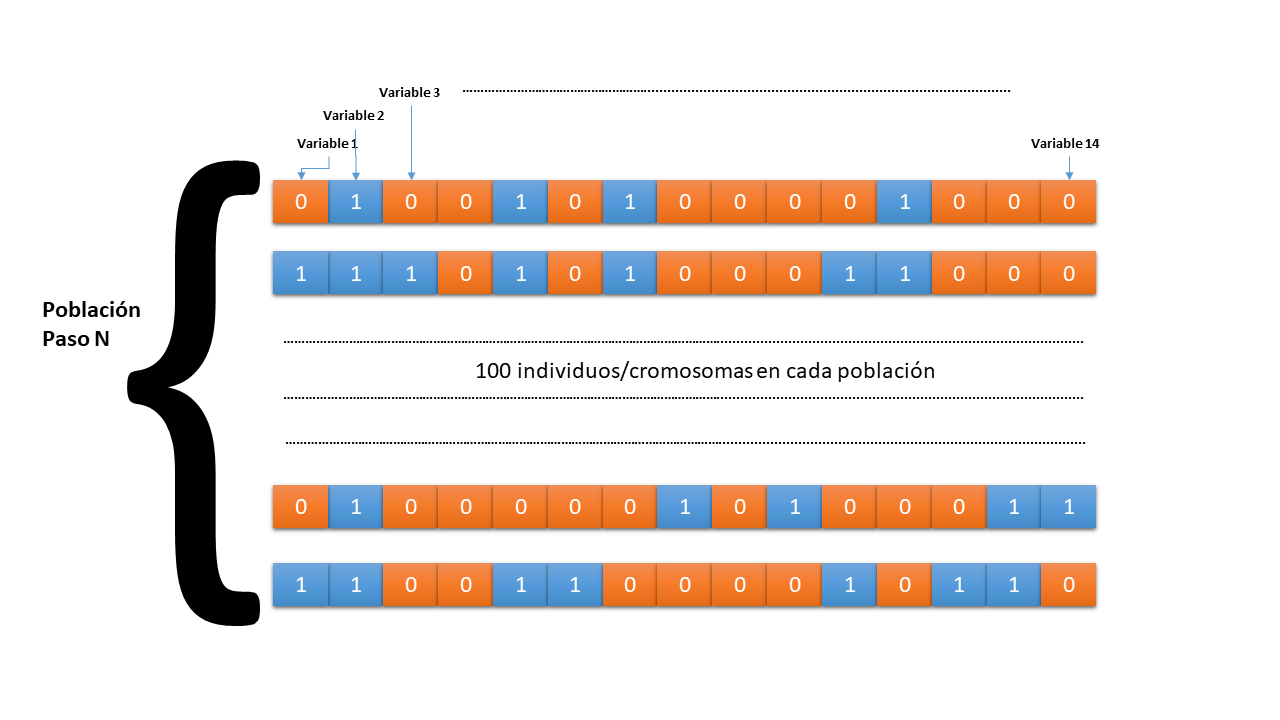
\includegraphics{imagenes/capitulo3/poblacion.png}

}

\caption{\label{fig-poblacion}Población en iteración N}

\end{figure}

\textbf{Función Fitness} (Evaluación)

Cuando estamos trabajando con selección de variables, el objetivo es
conseguir el conjunto de variables que mejor modelo construyan según
nuestro dataset. En este caso, al ser un problema de
\textbf{clasificación}, veremos cual es la combinación de variables que
nos da \textbf{menos errores al clasificar}.

Nuestra función fitness deberá seguir estos \textbf{pasos}:

- Recibe una \textbf{variable} llamada \textbf{indices} que tiene el
tamaño del numero de variables (el tamaño del cromosoma) que hay en el
dataframe (en nuestro caso 14) de datos.

\begin{itemize}
\tightlist
\item
  Los valores son \textbf{1} si esa variable se va a \textbf{usar} y
  \textbf{0} si \textbf{no} se va a \textbf{usar}.
\end{itemize}

- Se construye un \textbf{modelo}, en este caso usamos \textbf{LDA}
(Análisis Discriminante Lineal) con las \textbf{variables} que tienen
\textbf{valor 1}.

- Calculamos el \textbf{error} que queremos minimizar (número de fallos)

- Para este caso del LDA cogemos los valores \textbf{\$posterior} que
nos dan la probabilidad de cada clase para cada entrada de la muestra

- Calculamos cual es el \textbf{máximo} y así le asignamos esa
\textbf{clase} como su solución. También podríamos coger directamente el
valor de \$class con la clase dada como predicción.

- Verificamos cuantos hemos fallado y lo dividimos por el número de
muestras para ver el \textbf{porcentaje} de \textbf{fallos}

- Devolvemos el \textbf{porcentaje de fallos}. El resultado de la
ejecución del algoritmo evolutivo (rbga.bin())) nos dará un objeto del
que tendremos que obtener que variables son las que queremos usar.

Figure~\ref{fig-poblacion_final}

\begin{figure}

{\centering 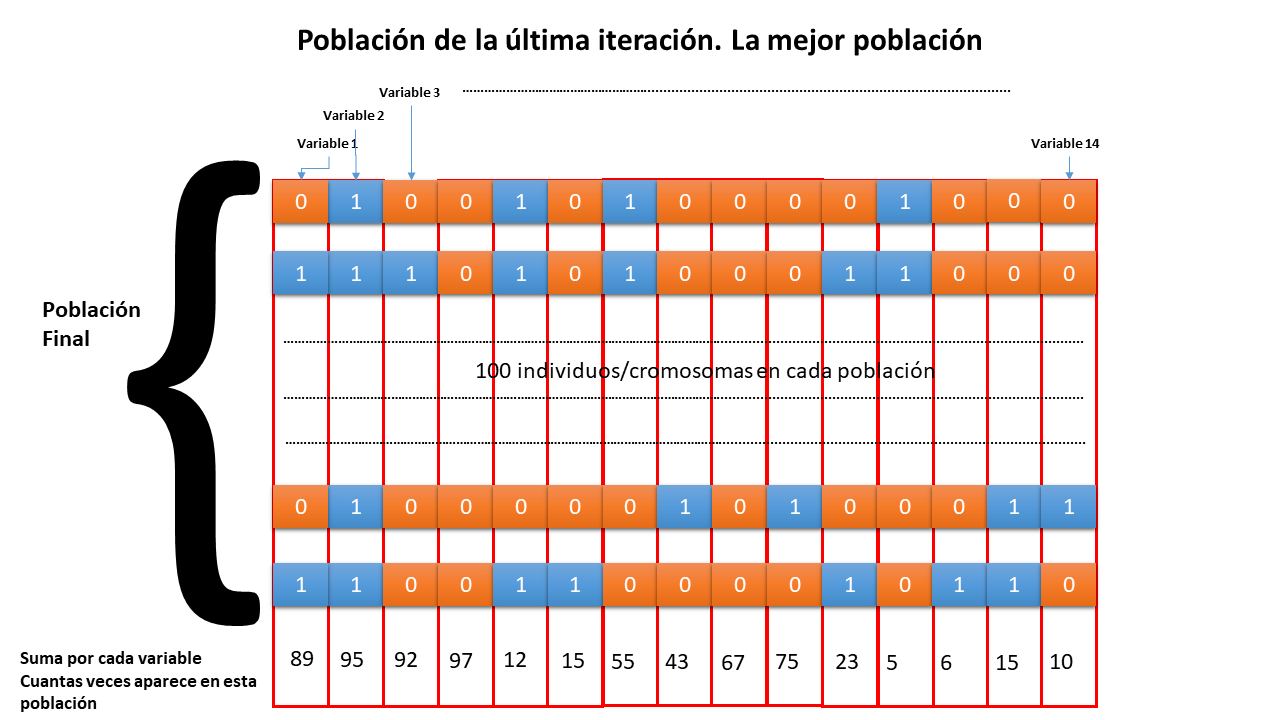
\includegraphics{imagenes/capitulo3/poblacion_final.png}

}

\caption{\label{fig-poblacion_final}Población Final}

\end{figure}

Una vez que nuestro algoritmo pare, deberíamos tener la población que
mejor se ha adaptado según el fitness que habíamos definido.

En nuestro caso estarán las 100 mejores combinaciones de variables, que
dan el menor error al clasificar. De esta manera si para cada variable
contamos cuantas veces ha salido en cada elemento de la población,
sabremos cuantas veces se ha usado en las combinaciones de variables de
esta última iteración (que es la mejor hasta ese momento). Con lo cual
podremos saber cuales han sido las \textbf{variables} \textbf{más}
\textbf{usadas} en la población final.

El objeto \textbf{modelo\_evolutivo}, que nos devuelve rbga.bin, tiene
una variable \textbf{population} de dimensiones tamaño\_población x
numero\_variables , en nuestro caso de 100x14, que tiene la información
de la población de la \textbf{última iteración del algoritmo}, que en un
principio debería ser la mejor. Este population contiene para cada fila
(elemento en la población), 0 o 1 en la posición que corresponde a cada
variable.

Para ver cuales son las variables que más se han usado tenemos que sumar
por columnas y ese dato nos dará para cada columna (corresponde con una
variable) la cantidad de veces que se ha usado en esta población. Una
vez tenemos estos datos ya podemos quedarnos con el número de variables
que deseemos cogiendo las que más alto valor tienen.

Algunos de los \textbf{parámetros} que tenemos que definir y que algunos
pueden afectar al rendimiento:

\begin{itemize}
\item
  \textbf{size:} Número de genes, en nuestro caso, número de variables
\item
  \textbf{popsize:} Tamaño de la población con la que se trabaja en cada
  iteración. Cuanto más alto sea este valor, más tiempo tardará la
  ejecución. En este caso vamos a usar 100 elementos en la población, es
  decir, en cada iteración habrá 100 combinaciones de variables.
\item
  \textbf{iters:} Número de iteraciones del algoritmo. Va a depender del
  problema pero seguramente entre 50 y 100 tendríamos una buena
  solución. Cuanto mayor sea esta variable, mayor será el tiempo de
  ejecución.
\item
  \textbf{zeroToOneRatio:} Con esta variable le indicamos al algoritmo
  cual es el ratio de ceros frente a unos cuando se generan elementos de
  la población, es decir, más o menos nos tiene que dar una idea de
  cuantas variables se van a usar a la vez (las que tienen unos).
  Podríamos estimar que si tenemos 14 variables y queremos reducir a
  tener alrededor de 4, deberíamos intentar en cada iteración tener un
  rango parecido a ese. La forma de conseguirlo sería poner un valor a
  esta variable de 1, es decir, cada 1 cero hay 1 uno. Lo que más o
  menos nos dejaría alrededor de 7 variables con 1. Como esto se genera
  de forma aleatoria, más o menos estaremos en un rango de variables
  útil parecido a lo que queremos.
\item
  \textbf{verbose:} Esta variable si la ponemos a TRUE se encargará de
  sacarnos información de la evolución del algoritmo. La recomendación
  es dejarla a FALSE ya que incrementa mucho el tiempo de ejecución.
\end{itemize}

\begin{longtable}[]{@{}l@{}}
\toprule\noalign{}
\endhead
\bottomrule\noalign{}
\endlastfoot
```r \\
 \\
``` \\
\end{longtable}

\begin{Shaded}
\begin{Highlighting}[numbers=left,,]
\FunctionTok{library}\NormalTok{(genalg) }\FunctionTok{library}\NormalTok{(MASS)}
\end{Highlighting}
\end{Shaded}

\begin{Shaded}
\begin{Highlighting}[numbers=left,,]
\FunctionTok{data}\NormalTok{(iris) }\FunctionTok{set.seed}\NormalTok{(}\DecValTok{999}\NormalTok{) }\CommentTok{\# Alas variables reales del dataset, les añadimos 10 variables más ficiticas (normal 0,1) \# Ponemos estas variables al principio X \textless{}{-} cbind(scale(iris[,1:4]),matrix(rnorm(10*150), 150, 10)) Y \textless{}{-} iris[,5]}
\end{Highlighting}
\end{Shaded}

\begin{Shaded}
\begin{Highlighting}[numbers=left,,]
\NormalTok{iris.evaluate }\OtherTok{\textless{}{-}} \ControlFlowTok{function}\NormalTok{(indices) \{}
\end{Highlighting}
\end{Shaded}

\begin{Shaded}
\begin{Highlighting}[numbers=left,,]
\NormalTok{result }\OtherTok{=} \DecValTok{1} \CommentTok{\# Tiene que haber al menos 2 variables if (sum(indices) \textgreater{} 2) \{}
\end{Highlighting}
\end{Shaded}

\begin{Shaded}
\begin{Highlighting}[numbers=left,,]
\CommentTok{\# Creamos un modelo de clasificación con LDA usando sólo las variables que vienen}
\CommentTok{\# marcadas en la variablindices con valor 1}
\CommentTok{\# El LDA tiene el valor $posterior que devuelve la probabilidad de cada clase (tenemos tres clases en Y)}
\CommentTok{\# Podríamos usar el valor de $class y así tendríamos directamente la clase.}
\NormalTok{modelo\_lda }\OtherTok{\textless{}{-}} \FunctionTok{lda}\NormalTok{(X[,indices}\SpecialCharTok{==}\DecValTok{1}\NormalTok{], Y, }\AttributeTok{CV=}\ConstantTok{TRUE}\NormalTok{)}\SpecialCharTok{$}\NormalTok{posterior}

\CommentTok{\# Cogemos la probabilidad más alta apply(modelo\_lda, 1,function(x)which(x == max(x))), para cada fila (150 muestras)}
\CommentTok{\# Comprobamos cuantos hemos fallado y lo dividimos por el tamaño de Y (150 muestras)}
\CommentTok{\# El objetivo es que sea mínimo este número de fallos}
\NormalTok{result }\OtherTok{=} \FunctionTok{sum}\NormalTok{(Y }\SpecialCharTok{!=} \FunctionTok{dimnames}\NormalTok{(modelo\_lda)[[}\DecValTok{2}\NormalTok{]][}\FunctionTok{apply}\NormalTok{(modelo\_lda, }\DecValTok{1}\NormalTok{,}\ControlFlowTok{function}\NormalTok{(x)}\FunctionTok{which}\NormalTok{(x }\SpecialCharTok{==} \FunctionTok{max}\NormalTok{(x)))]) }\SpecialCharTok{/} \FunctionTok{length}\NormalTok{(Y)}\ErrorTok{\}}
\end{Highlighting}
\end{Shaded}

\begin{Shaded}
\begin{Highlighting}[numbers=left,,]
\NormalTok{result }\ErrorTok{\}}
\end{Highlighting}
\end{Shaded}

\begin{Shaded}
\begin{Highlighting}[numbers=left,,]
\NormalTok{Ejecutamos el algoritmo evolutivo}
\end{Highlighting}
\end{Shaded}

\begin{Shaded}
\begin{Highlighting}[numbers=left,,]
\FunctionTok{system.time}\NormalTok{(\{ modelo\_evolutivo }\OtherTok{\textless{}{-}} \FunctionTok{rbga.bin}\NormalTok{(}\AttributeTok{size=}\DecValTok{14}\NormalTok{, }\AttributeTok{mutationChance=}\FloatTok{0.05}\NormalTok{, }\AttributeTok{zeroToOneRatio=}\DecValTok{1}\NormalTok{,}\AttributeTok{evalFunc=}\NormalTok{iris.evaluate, }\AttributeTok{verbose=}\ConstantTok{FALSE}\NormalTok{, }\AttributeTok{iters =} \DecValTok{50}\NormalTok{, }\AttributeTok{popSize =} \DecValTok{100}\NormalTok{) \}) }\DocumentationTok{\#\# user system elapsed \#\# 17.05 0.72 22.03}
\end{Highlighting}
\end{Shaded}

\begin{Shaded}
\begin{Highlighting}[numbers=left,,]
\NormalTok{Veamos como ha quedado el resultado de la población segúnla gráfica que nos da cuantas veces aparece cada variable en la población final. }\FunctionTok{library}\NormalTok{(ggplot2)}
\end{Highlighting}
\end{Shaded}

\begin{Shaded}
\begin{Highlighting}[numbers=left,,]
\NormalTok{Mostramos cual es el que ha aparecido más veces en la última iteración}
\end{Highlighting}
\end{Shaded}

\begin{Shaded}
\begin{Highlighting}[numbers=left,,]
\NormalTok{uso\_variables }\OtherTok{\textless{}{-}} \FunctionTok{colSums}\NormalTok{(modelo\_evolutivo}\SpecialCharTok{$}\NormalTok{population)}
\end{Highlighting}
\end{Shaded}

\begin{Shaded}
\begin{Highlighting}[numbers=left,,]
\NormalTok{Visualizamos cuanto se ha usado cada variable en esta última población}
\end{Highlighting}
\end{Shaded}

\begin{Shaded}
\begin{Highlighting}[numbers=left,,]
\NormalTok{Construimos un dataframe con los datos}
\end{Highlighting}
\end{Shaded}

\begin{Shaded}
\begin{Highlighting}[numbers=left,,]
\NormalTok{datos }\OtherTok{\textless{}{-}} \FunctionTok{data.frame}\NormalTok{(}\AttributeTok{variables=}\FunctionTok{c}\NormalTok{(}\DecValTok{1}\SpecialCharTok{:}\DecValTok{14}\NormalTok{),}\AttributeTok{uso=}\NormalTok{uso\_variables)}
\end{Highlighting}
\end{Shaded}

\begin{Shaded}
\begin{Highlighting}[numbers=left,,]
\FunctionTok{ggplot}\NormalTok{(datos,}\FunctionTok{aes}\NormalTok{(}\AttributeTok{x=}\NormalTok{variables,}\AttributeTok{y=}\NormalTok{uso, }\AttributeTok{fill=}\NormalTok{uso)) }\SpecialCharTok{+} \FunctionTok{geom\_bar}\NormalTok{(}\AttributeTok{stat=}\StringTok{"identity"}\NormalTok{) }\SpecialCharTok{+} \FunctionTok{theme\_minimal}\NormalTok{()}
\end{Highlighting}
\end{Shaded}

\begin{Shaded}
\begin{Highlighting}[numbers=left,,]
\NormalTok{Obtenemos ahora cuales son las variables con los valores más altos. Primero vemos las suma de las columnas, que nos dará los valores de cuantas veces aparece cada variable, y luego hacemos una función que nos dice cuales son las variables más usadas pasándole como parámetro el vector de uso\_variables y luego cuantas variables queremos quedarnos. }\CommentTok{\# Creamos una función que nos da de un vector los índices de posición \# donde están las X variables más usadas \# Le pasamos como parámetro el vector y cuantas variables queremos que devuelva}
\end{Highlighting}
\end{Shaded}

Figure~\ref{fig-frecuencia_variables}

Imagen \ref{fig-frecuencia_variables}

\begin{figure}

{\centering 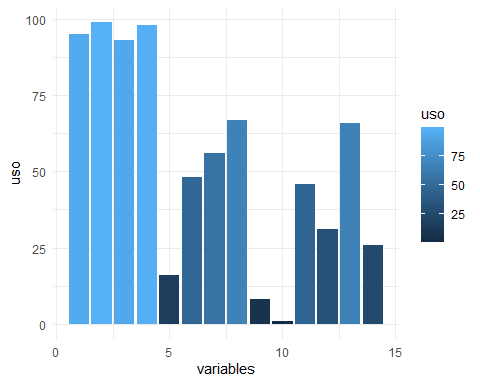
\includegraphics{imagenes/capitulo3/frecuencia_variables.png}

}

\caption{\label{fig-frecuencia_variables}Frecuencia de las Variables}

\end{figure}

\begin{Shaded}
\begin{Highlighting}[numbers=left,,]
\NormalTok{posicion\_maximos }\OtherTok{\textless{}{-}} \ControlFlowTok{function}\NormalTok{(datos, cuantos) \{ variables }\OtherTok{\textless{}{-}} \ConstantTok{NULL} \ControlFlowTok{if}\NormalTok{( cuantos}\SpecialCharTok{\textgreater{}}\DecValTok{0}\NormalTok{) \{ }\ControlFlowTok{for}\NormalTok{( i }\ControlFlowTok{in} \DecValTok{1}\SpecialCharTok{:}\NormalTok{cuantos ) \{ variables[i] }\OtherTok{\textless{}{-}} \FunctionTok{which.max}\NormalTok{(datos) datos[variables[i]] }\OtherTok{\textless{}{-}} \DecValTok{0}\NormalTok{ \}}
\end{Highlighting}
\end{Shaded}

\begin{Shaded}
\begin{Highlighting}[numbers=left,,]
\ErrorTok{\}}\NormalTok{ variables}
\end{Highlighting}
\end{Shaded}

\begin{Shaded}
\begin{Highlighting}[numbers=left,,]
\ErrorTok{\}}
\end{Highlighting}
\end{Shaded}

\begin{Shaded}
\begin{Highlighting}[numbers=left,,]
\NormalTok{Obtenemos ahora cuales son las }\DecValTok{6}\NormalTok{ variables más usados}
\end{Highlighting}
\end{Shaded}

\begin{Shaded}
\begin{Highlighting}[numbers=left,,]
\FunctionTok{posicion\_maximos}\NormalTok{(uso\_variables, }\DecValTok{6}\NormalTok{) }\DocumentationTok{\#\# [1] 2 4 1 3 8 13 }
\end{Highlighting}
\end{Shaded}

\hypertarget{algoritmos-genuxe9ticos-en-python}{%
\subsection{Algoritmos genéticos en
Python}\label{algoritmos-genuxe9ticos-en-python}}

\begin{Shaded}
\begin{Highlighting}[numbers=left,,]
\ImportTok{import}\NormalTok{ os }\ImportTok{import}\NormalTok{ pandas }\ImportTok{as}\NormalTok{ pd }\ImportTok{import}\NormalTok{ numpy }\ImportTok{as}\NormalTok{ np }\ImportTok{import}\NormalTok{ matplotlib.pyplot }\ImportTok{as}\NormalTok{ plt }\ImportTok{import}\NormalTok{ seaborn }\ImportTok{as}\NormalTok{ sns}

\ImportTok{from}\NormalTok{ genetic\_selection }\ImportTok{import}\NormalTok{ GeneticSelectionCV}

\ImportTok{from}\NormalTok{ sklearn.preprocessing }\ImportTok{import}\NormalTok{ StandardScaler }\ImportTok{from}\NormalTok{ sklearn.model\_selection }\ImportTok{import}\NormalTok{ train\_test\_split }\ImportTok{from}\NormalTok{ sklearn.metrics }\ImportTok{import}\NormalTok{ confusion\_matrix}
\end{Highlighting}
\end{Shaded}

\textbf{Cargar datos de trabajo}

\begin{Shaded}
\begin{Highlighting}[numbers=left,,]

\NormalTok{os.chdir(}\StringTok{\textquotesingle{}C:/Users/p\_san/Desktop/Máster\_2020/Módulo\_5\textquotesingle{}}\NormalTok{) }\CommentTok{\#directorio datos=pd.read\_csv(\textquotesingle{}german\_credit.csv\textquotesingle{},encoding = \textquotesingle{}ISO{-}8859{-}1\textquotesingle{}, index\_col=None)}
\end{Highlighting}
\end{Shaded}

Todas las variables son categóricas salvo:

duration

credit\_amount

residence\_since

age

existing\_credits

num\_dependents

Conversión a variables categóricas

\begin{Shaded}
\begin{Highlighting}[numbers=left,,]
\NormalTok{datos\textbackslash{}[}\StringTok{\textquotesingle{}checking\_status\textquotesingle{}}\NormalTok{\textbackslash{}]}\OperatorTok{=}\NormalTok{datos\textbackslash{}[}\StringTok{\textquotesingle{}checking\_status\textquotesingle{}}\NormalTok{\textbackslash{}].astype(}\StringTok{\textquotesingle{}category\textquotesingle{}}\NormalTok{) datos\textbackslash{}[}\StringTok{\textquotesingle{}credit\_history\textquotesingle{}}\NormalTok{\textbackslash{}]}\OperatorTok{=}\NormalTok{datos\textbackslash{}[}\StringTok{\textquotesingle{}credit\_history\textquotesingle{}}\NormalTok{\textbackslash{}].astype(}\StringTok{\textquotesingle{}category\textquotesingle{}}\NormalTok{) datos\textbackslash{}[}\StringTok{\textquotesingle{}purpose\textquotesingle{}}\NormalTok{\textbackslash{}]}\OperatorTok{=}\NormalTok{datos\textbackslash{}[}\StringTok{\textquotesingle{}purpose\textquotesingle{}}\NormalTok{\textbackslash{}].astype(}\StringTok{\textquotesingle{}category\textquotesingle{}}\NormalTok{) datos\textbackslash{}[}\StringTok{\textquotesingle{}savings\_status\textquotesingle{}}\NormalTok{\textbackslash{}]}\OperatorTok{=}\NormalTok{datos\textbackslash{}[}\StringTok{\textquotesingle{}savings\_status\textquotesingle{}}\NormalTok{\textbackslash{}].astype(}\StringTok{\textquotesingle{}category\textquotesingle{}}\NormalTok{) datos\textbackslash{}[}\StringTok{\textquotesingle{}employment\textquotesingle{}}\NormalTok{\textbackslash{}]}\OperatorTok{=}\NormalTok{datos\textbackslash{}[}\StringTok{\textquotesingle{}employment\textquotesingle{}}\NormalTok{\textbackslash{}].astype(}\StringTok{\textquotesingle{}category\textquotesingle{}}\NormalTok{) datos\textbackslash{}[}\StringTok{\textquotesingle{}personal\_status\textquotesingle{}}\NormalTok{\textbackslash{}]}\OperatorTok{=}\NormalTok{datos\textbackslash{}[}\StringTok{\textquotesingle{}personal\_status\textquotesingle{}}\NormalTok{\textbackslash{}].astype(}\StringTok{\textquotesingle{}category\textquotesingle{}}\NormalTok{) datos\textbackslash{}[}\StringTok{\textquotesingle{}other\_parties\textquotesingle{}}\NormalTok{\textbackslash{}]}\OperatorTok{=}\NormalTok{datos\textbackslash{}[}\StringTok{\textquotesingle{}other\_parties\textquotesingle{}}\NormalTok{\textbackslash{}].astype(}\StringTok{\textquotesingle{}category\textquotesingle{}}\NormalTok{) datos\textbackslash{}[}\StringTok{\textquotesingle{}property\_magnitude\textquotesingle{}}\NormalTok{\textbackslash{}]}\OperatorTok{=}\NormalTok{datos\textbackslash{}[}\StringTok{\textquotesingle{}property\_magnitude\textquotesingle{}}\NormalTok{\textbackslash{}].astype(}\StringTok{\textquotesingle{}category\textquotesingle{}}\NormalTok{) datos\textbackslash{}[}\StringTok{\textquotesingle{}other\_payment\_plans\textquotesingle{}}\NormalTok{\textbackslash{}]}\OperatorTok{=}\NormalTok{datos\textbackslash{}[}\StringTok{\textquotesingle{}other\_payment\_plans\textquotesingle{}}\NormalTok{\textbackslash{}].astype(}\StringTok{\textquotesingle{}category\textquotesingle{}}\NormalTok{) datos\textbackslash{}[}\StringTok{\textquotesingle{}housing\textquotesingle{}}\NormalTok{\textbackslash{}]}\OperatorTok{=}\NormalTok{datos\textbackslash{}[}\StringTok{\textquotesingle{}housing\textquotesingle{}}\NormalTok{\textbackslash{}].astype(}\StringTok{\textquotesingle{}category\textquotesingle{}}\NormalTok{) datos\textbackslash{}[}\StringTok{\textquotesingle{}job\textquotesingle{}}\NormalTok{\textbackslash{}]}\OperatorTok{=}\NormalTok{datos\textbackslash{}[}\StringTok{\textquotesingle{}job\textquotesingle{}}\NormalTok{\textbackslash{}].astype(}\StringTok{\textquotesingle{}category\textquotesingle{}}\NormalTok{) datos\textbackslash{}[}\StringTok{\textquotesingle{}property\_magnitude\textquotesingle{}}\NormalTok{\textbackslash{}]}\OperatorTok{=}\NormalTok{datos\textbackslash{}[}\StringTok{\textquotesingle{}property\_magnitude\textquotesingle{}}\NormalTok{\textbackslash{}].astype(}\StringTok{\textquotesingle{}category\textquotesingle{}}\NormalTok{) datos\textbackslash{}[}\StringTok{\textquotesingle{}own\_telephone\textquotesingle{}}\NormalTok{\textbackslash{}]}\OperatorTok{=}\NormalTok{datos\textbackslash{}[}\StringTok{\textquotesingle{}own\_telephone\textquotesingle{}}\NormalTok{\textbackslash{}].astype(}\StringTok{\textquotesingle{}category\textquotesingle{}}\NormalTok{) datos\textbackslash{}[}\StringTok{\textquotesingle{}foreign\_worker\textquotesingle{}}\NormalTok{\textbackslash{}]}\OperatorTok{=}\NormalTok{datos\textbackslash{}[}\StringTok{\textquotesingle{}foreign\_worker\textquotesingle{}}\NormalTok{\textbackslash{}].astype(}\StringTok{\textquotesingle{}category\textquotesingle{}}\NormalTok{) datos\textbackslash{}[}\StringTok{\textquotesingle{}class\textquotesingle{}}\NormalTok{\textbackslash{}]}\OperatorTok{=}\NormalTok{datos\textbackslash{}[}\StringTok{\textquotesingle{}class\textquotesingle{}}\NormalTok{\textbackslash{}].astype(}\StringTok{\textquotesingle{}category\textquotesingle{}}\NormalTok{)}
\end{Highlighting}
\end{Shaded}

La variable class es una variable reservada en diferentes módulos de
Python -\textgreater{} reemplazar por por target

\begin{Shaded}
\begin{Highlighting}[numbers=left,,]
\NormalTok{datos.rename(columns}\OperatorTok{=}\NormalTok{\{}\StringTok{\textquotesingle{}class\textquotesingle{}}\NormalTok{: }\StringTok{\textquotesingle{}target\textquotesingle{}}\NormalTok{\}, inplace}\OperatorTok{=}\VariableTok{True}\NormalTok{) datos\textbackslash{}[}\StringTok{\textquotesingle{}target\textquotesingle{}}\NormalTok{\textbackslash{}]}\OperatorTok{=}\NormalTok{np.where(datos\textbackslash{}[}\StringTok{\textquotesingle{}target\textquotesingle{}}\NormalTok{\textbackslash{}]}\OperatorTok{==}\StringTok{\textquotesingle{}good\textquotesingle{}}\NormalTok{, }\DecValTok{0}\NormalTok{, }\DecValTok{1}\NormalTok{) \textbackslash{}}\CommentTok{\# cambio en la codificación por sencillez en el preprocesado}
\end{Highlighting}
\end{Shaded}

Definición de la muestra de trabajo

\begin{Shaded}
\begin{Highlighting}[numbers=left,,]
\NormalTok{datos\_entrada}\OperatorTok{=}\NormalTok{datos.drop(}\StringTok{\textquotesingle{}target\textquotesingle{}}\NormalTok{, axis}\OperatorTok{=}\DecValTok{1}\NormalTok{) \textbackslash{}}\CommentTok{\# Datos de entrada datos\_entrada= pd.get\_dummies(datos\_entrada, drop\_first=True) \#conversión a variables dummy}
\end{Highlighting}
\end{Shaded}

datos de salida

\begin{Shaded}
\begin{Highlighting}[numbers=left,,]
\NormalTok{respuesta}\OperatorTok{=}\NormalTok{datos.loc\textbackslash{}[:, }\StringTok{\textquotesingle{}target\textquotesingle{}}\NormalTok{\textbackslash{}]}
\end{Highlighting}
\end{Shaded}

Escalado de las variables, partición de la muestra y Cross Validation

\begin{Shaded}
\begin{Highlighting}[numbers=left,,]
\NormalTok{seed}\OperatorTok{=}\DecValTok{123}\NormalTok{ \textbackslash{}}\CommentTok{\# Escalado de los datos de entrada x\_esc=StandardScaler().fit\_transform(datos\_entrada) x\_esc=pd.DataFrame(x\_esc, columns=datos\_entrada.columns)}
\end{Highlighting}
\end{Shaded}

Partición de la muestra

test\_size=0.3 \#muestra para el test x\_train, x\_test, y\_train,
y\_test = train\_test\_split(x\_esc,respuesta, test\_size=test\_size,
random\_state=seed, stratify=respuesta) Usando un modelo Cart from
sklearn.tree import DecisionTreeClassifier
cart=DecisionTreeClassifier(max\_depth=5, random\_state=seed)
cart\_algoritmo\_gen=GeneticSelectionCV(cart, cv=5, \# 5 particiones
verbose=0, \# no se muestran los resultados en la pantalla
scoring=``roc\_auc'', \# ejemplo métrica para evaluar max\_features=15,
\# número de variables máximas en la selección de\\
\# características n\_population=50, \# tamaño de la población
crossover\_proba=0.5, \# probabilidad de cruce entre parejas de genes
mutation\_proba=0.2, \#probabilidad de mutación n\_generations=40,
\#número de generaciones crossover\_independent\_proba=0.5, \# prob.
cruce para genes \# independientes mutation\_independent\_proba=0.05, \#
prob. mutación de genes \# independientes tournament\_size=3, \#tamaño
de los grupos n\_gen\_no\_change=10, \# genes que se mantienen
-\textgreater{} no pasan a \# la segunda generación caching=True,
n\_jobs=1)

cart\_algoritmo\_gen=cart\_algoritmo\_gen.fit(x\_train, y\_train)\\
ajuste del modelo usando algoritmo genéticos para la selección de
variables \# Variables Seleccionadas print(`Num. Var:',
cart\_algoritmo\_gen.n\_features\_) \#
print(cart\_algoritmo\_gen.support\_)\\
\# Resultados matriz numpy -\textgreater{} mala visualización. Los
resultados se \# convierten a df de pandas
df=pd.DataFrame(cart\_algoritmo\_gen.support\_,
columns={[}`Variables'{]}, index=x\_train.columns)
df=df.loc{[}\textasciitilde df{[}`Variables'{]}.isin({[}False{]}){]}
\#se elimina del df las variables no seleccionadas por el algoritmo
list(df.index) \# variables seleccionadas por el algoritmo

Num. Var: 9 {[}`checking\_status\_0\textless=X\textless200',
`checking\_status\_\textless0', ``credit\_history\_`critical/other
existing credit'\,'', ``purpose\_`used car'\,'',
`savings\_status\_\textgreater=1000', ``personal\_status\_`male
single'\,'', `other\_parties\_guarantor',
`other\_payment\_plans\_stores', `job\_skilled'{]}

Resultados test - predicción \& Matriz de confusión (modelo CART con
selección de variables a través de Algoritmos Genéticos)

pred=cart\_algoritmo\_gen.predict(x\_test)

confusion\_matrix(y\_test, pred) \# Matriz de confusión

array({[}{[}173, 37{]}, {[} 46, 44{]}{]}, dtype=int64)

\bookmarksetup{startatroot}

\hypertarget{luxf3gica-difusa}{%
\chapter{Lógica Difusa}\label{luxf3gica-difusa}}

\hypertarget{conceptos-clave.}{%
\section{Conceptos clave.}\label{conceptos-clave.}}

\hypertarget{conjuntos-difusos-y-funciones-de-membresuxeda}{%
\subsection{Conjuntos difusos y funciones de
membresía}\label{conjuntos-difusos-y-funciones-de-membresuxeda}}

\hypertarget{inferencia-y-modelamiento-difuso}{%
\subsection{Inferencia y Modelamiento
difuso}\label{inferencia-y-modelamiento-difuso}}

\hypertarget{ejemplos-pruxe1cticos-1}{%
\section{Ejemplos prácticos}\label{ejemplos-pruxe1cticos-1}}

\hypertarget{clustering-difuso}{%
\subsection{Clustering Difuso}\label{clustering-difuso}}

\hypertarget{herramientas-de-diagnuxf3stico}{%
\subsection{Herramientas de
Diagnóstico}\label{herramientas-de-diagnuxf3stico}}

\bookmarksetup{startatroot}

\hypertarget{bibliografia}{%
\chapter*{Bibliografia}\label{bibliografia}}
\addcontentsline{toc}{chapter}{Bibliografia}

\markboth{Bibliografia}{Bibliografia}

\hypertarget{refs}{}
\begin{CSLReferences}{1}{0}
\leavevmode\vadjust pre{\hypertarget{ref-knuth84}{}}%
Knuth, Donald E. 1984. {``Literate Programming.''} \emph{Comput. J.} 27
(2): 97--111. \url{https://doi.org/10.1093/comjnl/27.2.97}.

\end{CSLReferences}

\cleardoublepage
\phantomsection
\addcontentsline{toc}{part}{Appendices}
\appendix

\hypertarget{anexo-1}{%
\chapter{Anexo 1}\label{anexo-1}}

Anexo 1



\printindex

\end{document}
